% options are:
% PhD, MSc (choose one)
% beforeExam (to make the personal thanks invisible)
\documentclass[MSc]{iitcsthesis}

\usepackage{times}
\usepackage{latexsym}
\usepackage{graphicx} % more modern
\usepackage{graphics}
\usepackage{subfigure}
\usepackage{natbib}

\usepackage{algorithm}
\usepackage{hyperref}

\usepackage{amsfonts}
\usepackage{amsmath}
\usepackage{amstext}
\usepackage{latexsym}
\usepackage{amssymb}
\setcounter{tocdepth}{3}
\usepackage{epstopdf}
\usepackage{url}
\usepackage{color}
\usepackage{wrapfig}
\usepackage{fancyvrb}
\usepackage{rotating}
\usepackage{enumerate}
\usepackage{tabulary}


% For some reason, the hebrew package clashes with the amsthm package. If you need a proof environment, you can uncomment the following:
%\usepackage{amssymb} %Needed for \blacksquare. Take care not to add this package twice...
%\newenvironment{proof}[1][Proof]{\par \textbf{#1.} }{\hspace{10pt}\hfill$\blacksquare$\par}
\begin{document}

\authorEnglish{Edward Moroshko}

\titleEnglish{New Min-Max Algorithms and Analysis for Online Regression}

\supervisorEnglish{The Research Thesis Was Done Under The Supervision
of Prof.~Koby Crammer in the Faculty of Electrical Engineering.}

\PublicationEnglish{\\Parts of this work were published in
\\Weighted Last-Step Min-Max Algorithm with Improved Sub-Logarithmic Regret.
\\Edward Moroshko and Koby Crammer. 2012. In ALT.
\\A Last-Step Regression Algorithm for Non-Stationary Online Learning.
\\Edward Moroshko and Koby Crammer. 2013. In AISTATS.}

\GregorianDateEnglish{June 2013}
\JewishDateEnglish{Tammuz, 5773}

\personalThanksEnglish{I would like to thank Koby for his remarkable guidance and support. I also thank Koby for funding my travels to ALT 2012 and AISTATS 2013 conferences.\\
Thanks to my family for the support.\\
Special thanks to my fiancee Ephrath for her love, support and patience along the way.
}
%\financialThanksEnglish{The generous financial support of the Technion is gratefully acknowledged.}

\maketitleEnglish

% The English abstract should be 200-500 words long.
\abstractEnglish
In online learning the performance of an algorithm is typically compared to the performance of a fixed function from some class, using a quantity called regret. The purpose of a learning algorithm is to have a regret as small as possible. About a decade ago, the last-step min-max approach has been proposed for online regression, where the algorithm tries to minimize the maximal (worst-case) regret with respect to the best-performing linear function.
In fact, to make the min-max optimization problem well defined it has been assumed that the choices of the adversary are bounded, yielding artificially only extreme cases. In this work we introduce a new algorithm that weighs the examples in such a way that the min-max problem will be well defined. We provide analysis of the algorithm and develop new regret bounds that are better in some situations than other state-of-the-art bounds.

In many real-world problems there is no fixed best target function during the runtime of the algorithm. Instead, the best (local) target function is drifting over time. In this work we extend the last-step min-max approach to the drifting setting and introduce a new algorithm which is a last-step min-max optimal in context of a drift. We analyze the algorithm in the worst-case regret framework and show that it maintains an average loss close to that of the best slowly changing sequence of linear functions, as long as the total of drift is sublinear. We show formally that in some situations our bound is better than existing bounds, and
%We also rely on the $H_\infty$ filter and its bound, and develop and analyze another algorithm for the drifting setting.
synthetic simulations demonstrate the advantages of our algorithm over previous approaches, especially in a worst-case constant drift setting.

%
%  Macros for Thesis
%%%%%%%%%%%%%%%%%%%%%%%%%%%%%%%%%%%%%%%%%%%%%%%%%%%%%%%%%%%%%%%%%%%%%%%%%%%%%

 \newtheorem{theorem}{Theorem}
 \newtheorem{lemma}[theorem]{Lemma}
 \newtheorem{definition}[theorem]{Definition}
% \newtheorem{claim}[theorem]{Claim}
 \newtheorem{corollary}[theorem]{Corollary}


%\newtheorem{theorem}{Theorem}
%\newtheorem{lemma}[theorem]{Lemma}
%\newtheorem{corollary}[theorem]{Corollary}
%\newtheorem{definition}{Definition}
\newtheorem{Remark}{Remark}
%\newtheorem{claim}{Claim}
%\def\blackslug{\hbox{\hskip 1pt \vrule width 4pt height 8pt depth 1.5pt
%\hskip 1pt}}
\def\proof{\par\penalty-1000\vskip .5 pt\noindent{\bf Proof\/: }}
%\def\myproof{\par\penalty-1000\vskip .5 pt\noindent{\bf Proof~}}
\def\proofsketch{\par\penalty-1000\vskip .5 pt\noindent{\bf Proof sketch\/: }}
%\newcommand{\QED}{\hfill$\;\;\;\rule[0.1mm]{2mm}{2mm}$}
%\def\Proof{\par\penalty-1000\vskip .5 pt\noindent{\bf Proof\/: }}
\def\ProofSketch{\par\penalty-1000\vskip .1 pt\noindent{\bf Proof sketch\/: }}
\newcommand{\QED}{\hfill$\;\;\;\rule[0.1mm]{2mm}{2mm}$\\}
%\newenvironment{Proof}{{\bf Proof:}}{\noindent\bbox\vspace{0.1in}}

\newcommand{\todo}[1]{{~\\\bf TODO: {#1}}~\\}

%%%%%%%%%%%%%%%%%%%%%%%%%%%%%%%%%%%%%%%%%%%%%%%%%%%%%%%%%%%%%%%%%%
% General
%%%%%%%%%%%%%%%%%%%%%%%%%%%%%%%%%%%%%%%%%%%%%%%%%%%%%%%%%%%%%%%%%%
\newfont{\msym}{msbm10}
\newcommand{\reals}{\mathbb{R}}%Re}%{mbox{\msym R}}
\newcommand{\half}{\frac{1}{2}}
\newcommand{\sign}{{\rm sign}}
\newcommand{\paren}[1]{\left({#1}\right)}
\newcommand{\brackets}[1]{\left[{#1}\right]}
\newcommand{\braces}[1]{\left\{{#1}\right\}}
\newcommand{\ceiling}[1]{\left\lceil{#1}\right\rceil}
\newcommand{\abs}[1]{\left\vert{#1}\right\vert}
\newcommand{\tr}{{\rm Tr}}
\newcommand{\pr}[1]{{\rm Pr}\left[{#1}\right]}
\newcommand{\prp}[2]{{\rm Pr}_{#1}\left[{#2}\right]}
\newcommand{\Exp}[1]{{\rm E}\left[{#1}\right]}
\newcommand{\Expp}[2]{{\rm E}_{#1}\left[{#2}\right]}
\newcommand{\eqdef}{\stackrel{\rm def}{=}}
\newcommand{\comdots}{, \ldots ,}
\newcommand{\true}{\texttt{True}}
\newcommand{\false}{\texttt{False}}
\newcommand{\mcal}[1]{{\mathcal{#1}}}
\newcommand{\argmin}[1]{\underset{#1}{\mathrm{argmin}} \:}
\newcommand{\normt}[1]{\left\Vert {#1} \right\Vert^2}
\newcommand{\step}[1]{\left[#1\right]_+}
\newcommand{\1}[1]{[\![{#1}]\!]}
\newcommand{\diag}{{\textrm{diag}}}
%\newcommand{\det}{{\textrm{det}}}
\newcommand{\KL}{{\textrm{D}_{\textrm{KL}}}}
\newcommand{\IS}{{\textrm{D}_{\textrm{IS}}}}
\newcommand{\EU}{{\textrm{D}_{\textrm{EU}}}}

%%%%%%%%%%%%%%%%%%%%%%%%%%%%%%%%%%%%%%%%%%%%%%%%%%%%%%%%%%
% Control symbols
%%%%%%%%%%%%%%%%%%%%%%%%%%%%%%%%%%%%%%%%%%%%%%%%%%%%%%%%%%
\newcommand{\leftmarginpar}[1]{\marginpar[#1]{}}
\newcommand{\figline}{\rule{0.50\textwidth}{0.5pt}}
\newcommand{\pseudocodefont}{\normalsize}
\newcommand{\nolineskips}{
\setlength{\parskip}{0pt}
\setlength{\parsep}{0pt}
\setlength{\topsep}{0pt}
\setlength{\partopsep}{0pt}
\setlength{\itemsep}{0pt}}

%%%%%%%%%%%%%%%%%%%%%%%%%%%%%%%%%%%%%%%%%%%%%%%%%%%%%%%%%%%
% Equations and references
%%%%%%%%%%%%%%%%%%%%%%%%%%%%%%%%%%%%%%%%%%%%%%%%%%%%%%%%%%%
\newcommand{\beq}[1]{\begin{equation}\label{#1}}
\newcommand{\eeq}{\end{equation}}
\newcommand{\beqa}{\begin{eqnarray}}
\newcommand{\eeqa}{\end{eqnarray}}
\renewcommand{\eqref}[1]{Eq.~(\ref{#1})}
\newcommand{\secref}[1]{Sec.~\ref{#1}}
\newcommand{\figref}[1]{Fig.~\ref{#1}}
\newcommand{\exmref}[1]{Example~\ref{#1}}
\newcommand{\thmref}[1]{Theorem~\ref{#1}}
\newcommand{\sthmref}[1]{Thm.~\ref{#1}}
\newcommand{\defref}[1]{Definition~\ref{#1}}
\newcommand{\remref}[1]{Remark~\ref{#1}}
\newcommand{\chapref}[1]{Chapter~\ref{#1}}
\newcommand{\appref}[1]{Appendix~\ref{#1}}
\newcommand{\lemref}[1]{Lemma~\ref{#1}}
\newcommand{\propref}[1]{Proposition~\ref{#1}}
\newcommand{\claimref}[1]{Claim~\ref{#1}}
\newcommand{\corref}[1]{Corollary~\ref{#1}}
\newcommand{\scorref}[1]{Cor.~\ref{#1}}
\newcommand{\tabref}[1]{Table~\ref{#1}}
\newcommand{\tran}[1]{{#1}^{\top}}
\newcommand{\norm}{\mcal{N}}
\newcommand{\eqsref}[1]{Eqns.~(\ref{#1})}
\newcommand{\algoref}[1]{Alg.~\ref{#1}}

%%%%%%%%%%%%%%%%%%%%%%%%%%%%%%%%%%%%%%%%%%%%%%%%%%%%%%%%%%%
% bold, up, down
%%%%%%%%%%%%%%%%%%%%%%%%%%%%%%%%%%%%%%%%%%%%%%%%%%%%%%%%%%%
\newcommand{\mb}[1]{{\boldsymbol{#1}}}
\newcommand{\up}[2]{{#1}^{#2}}
\newcommand{\dn}[2]{{#1}_{#2}}
\newcommand{\du}[3]{{#1}_{#2}^{#3}}
\renewcommand{\star}[1]{\up{#1}{*}}
\newcommand{\textl}[2]{{$\textrm{#1}_{\textrm{#2}}$}}


%%%%%%%%%%%%%%%%%%%%%%%%%%%%%%%%%%%%%%%%%%%%%%%%%%%%%%%%%%%
% vectors \va
%%%%%%%%%%%%%%%%%%%%%%%%%%%%%%%%%%%%%%%%%%%%%%%%%%%%%%%%%%%
\newcommand{\vx}{\mathbf{x}}
\newcommand{\vxi}[1]{\vx_{#1}}
\newcommand{\vxii}{\vxi{t}}

\newcommand{\ve}{\mathbf{e}}
\newcommand{\vei}[1]{\ve_{#1}}
\newcommand{\veii}{\vei{t}}
\newcommand{\vet}{\ve^{\top}}
\newcommand{\veti}[1]{\vet_{#1}}
\newcommand{\vetii}{\veti{i}}
\newcommand{\yi}[1]{y_{#1}}
\newcommand{\yii}{\yi{t}}
\newcommand{\hyi}[1]{\hat{y}_{#1}}
\newcommand{\hyii}{\hyi{i}}

\newcommand{\vy}{\mb{y}}
\newcommand{\vyi}[1]{\vy_{#1}}
\newcommand{\vyii}{\vyi{i}}

\newcommand{\vn}{\mb{\nu}}
\newcommand{\vni}[1]{\vn_{#1}}
\newcommand{\vnii}{\vni{i}}

\newcommand{\tvn}{\tilde{\mb{\nu}}}

\newcommand{\vmu}{\mb{\mu}}
\newcommand{\vmus}{{\vmu^*}}
\newcommand{\vmuts}{{\vmus}^{\top}}
\newcommand{\vmui}[1]{\vmu_{#1}}
\newcommand{\vmuii}{\vmui{i}}

\newcommand{\vmut}{\vmu^{\top}}
\newcommand{\vmuti}[1]{\vmut_{#1}}
\newcommand{\vmutii}{\vmuti{i}}

\newcommand{\vsigma}{\mb \sigma}
\newcommand{\msigma}{\mathbf{\Sigma}}
\newcommand{\msigmas}{{\msigma^*}}
\newcommand{\msigmai}[1]{\msigma_{#1}}
\newcommand{\msigmaii}{\msigmai{t}}

\newcommand{\mups}{\Upsilon}
\newcommand{\mupss}{{\mups^*}}
\newcommand{\mupsi}[1]{\mups_{#1}}
\newcommand{\mupsii}{\mupsi{i}}
\newcommand{\upssl}{\upsilon^*_l}


\newcommand{\vu}{\mathbf{u}}
\newcommand{\vut}{\tran{\vu}}
\newcommand{\vui}[1]{\vu_{#1}}
\newcommand{\vuti}[1]{\vut_{#1}}
\newcommand{\hvu}{\hat{\vu}}
\newcommand{\hvut}{\tran{\hvu}}
\newcommand{\hvur}[1]{\hvu_{#1}}
\newcommand{\hvutr}[1]{\hvut_{#1}}
\newcommand{\vw}{\mathbf{w}}
\newcommand{\vwi}[1]{\vw_{#1}}
\newcommand{\vwii}{\vwi{t}}
\newcommand{\vwti}[1]{\vwt_{#1}}
\newcommand{\vwt}{\tran{\vw}}

\newcommand{\tvw}{\tilde{\mathbf{w}}}
\newcommand{\tvwi}[1]{\tvw_{#1}}
\newcommand{\tvwii}{\tvwi{t}}

\newcommand{\vh}{\mb{h}}

\newcommand{\vv}{\mb{v}}
\newcommand{\vvt}{\tran{\vv}}

\newcommand{\vvi}[1]{\vv_{#1}}
\newcommand{\vvti}[1]{\vvt_{#1}}
\newcommand{\lambdai}[1]{\lambda_{#1}}
\newcommand{\Lambdai}[1]{\Lambda_{#1}}

\newcommand{\vxt}{\tran{\vx}}
\newcommand{\vxiit}{\vxi{i,t}}
\newcommand{\hvx}{\hat{\vx}}
\newcommand{\hvxi}[1]{\hvx_{#1}}
\newcommand{\hvxii}{\hvxi{i}}
\newcommand{\hvxt}{\tran{\hvx}}
\newcommand{\hvxti}[1]{\hvxt_{#1}}
\newcommand{\hvxtii}{\hvxti{i}}
\newcommand{\vxti}[1]{\vxt_{#1}}
\newcommand{\vxtii}{\vxti{i}}
\newcommand{\vwiit}{\vwi{i,t}}

\newcommand{\vb}{\mb{b}}
\newcommand{\vbt}{\tran{\vb}}
\newcommand{\vbi}[1]{\vb_{#1}}


\newcommand{\hvy}{\hat{\vy}}
\newcommand{\hvyi}[1]{\hvy_{#1}}
\newcommand{\yiit}{\yi{i,t}}

%%%%%%%%%%%%%%%%%%%%%%%%%%%%%%%%%%%%%%%%%%%%%%%%%%%%%%%%%%%%%%%%%
% Matrices (\mA)
%%%%%%%%%%%%%%%%%%%%%%%%%%%%%%%%%%%%%%%%%%%%%%%%%%%%%%%%%%%%%%%%%


\renewcommand{\mp}{P}
\newcommand{\mpd}{\mp^{(d)}}
\newcommand{\mpt}{\mp^T}
\newcommand{\tmp}{\tilde{\mp}}
\newcommand{\mpi}[1]{\mp_{#1}}
\newcommand{\mpti}[1]{\mpt_{#1}}
\newcommand{\mptii}{\mpti{i}}
\newcommand{\mpii}{\mpi{i}}
\newcommand{\mps}{Q}
\newcommand{\mpsi}[1]{\mps_{#1}}
\newcommand{\mpsii}{\mpsi{i}}
\newcommand{\tmpt}{\tmp^T}
\newcommand{\mz}{Z}
\newcommand{\mv}{V}
\newcommand{\mvi}[1]{\mv_{#1}}
\newcommand{\mvt}{V^T}
\newcommand{\mvti}[1]{\mvt_{#1}}
\newcommand{\mzt}{\mz^T}
\newcommand{\tmz}{\tilde{\mz}}
\newcommand{\tmzt}{\tmz^T}
\newcommand{\mx}{\mathbf{X}}
\newcommand{\ma}{\mathbf{A}}
\newcommand{\mxs}[1]{\mx_{#1}}


\newcommand{\mai}[1]{\ma_{#1}}
\newcommand{\mat}{\tran{\ma}}
\newcommand{\mati}[1]{\mat_{#1}}

\newcommand{\mc}{{C}}
\newcommand{\mci}[1]{\mc_{#1}}
\newcommand{\mcti}[1]{\mct_{#1}}


\newcommand{\md}{{\mathbf{D}}}
\newcommand{\mdi}[1]{\md_{#1}}
\newcommand{\mxi}[1]{\textrm{diag}^2\paren{\vxi{#1}}}
\newcommand{\mxii}{\mxi{i}}

%\newcommand{\mxi}[1]{\mx_{#1}}
%\newcommand{\mxii}{\mxi{i}}
\newcommand{\hmx}{\hat{\mx}}
\newcommand{\hmxi}[1]{\hmx_{#1}}
\newcommand{\hmxii}{\hmxi{i}}
\newcommand{\hmxt}{\hmx^T}
\newcommand{\mxt}{\mx^\top}
\newcommand{\mi}{\mathbf{I}}
\newcommand{\mq}{Q}
\newcommand{\mqt}{\mq^T}
\newcommand{\mlam}{\Lambda}
%\newcommand{\ma}{A}
%\newcommand{\ms}{S}
%\newcommand{\mt}{T}

%%%%%%%%%%%%%%%%%%%%%%%%%%%%%%%%%%%%%%%%%%%%%%%%%%%%%%%%%%%
% mathcal
%%%%%%%%%%%%%%%%%%%%%%%%%%%%%%%%%%%%%%%%%%%%%%%%%%%%%%%%%%%
\renewcommand{\L}{\mcal{L}}
%\newcommand{\R}{\mcal{R}}
\newcommand{\X}{\mcal{X}}
\newcommand{\Y}{\mcal{Y}}
\newcommand{\F}{\mcal{F}}
\newcommand{\nur}[1]{\nu_{#1}}
\newcommand{\lambdar}[1]{\lambda_{#1}}
\newcommand{\gammai}[1]{\gamma_{#1}}
\newcommand{\gammaii}{\gammai{i}}
\newcommand{\alphai}[1]{\alpha_{#1}}
\newcommand{\alphaii}{\alphai{i}}
\newcommand{\lossp}[1]{\ell_{#1}}
\newcommand{\eps}{\epsilon}
\newcommand{\epss}{\eps^*}
\newcommand{\lsep}{\lossp{\eps}}
\newcommand{\lseps}{\lossp{\epss}}
\newcommand{\T}{\mcal{T}}

%%%%%%%%%%%%%%%%%%%%%%%%%%%%%%%%%%%%%%%%%%%%%%%%%%%%%%%%%%%
% Notes
%%%%%%%%%%%%%%%%%%%%%%%%%%%%%%%%%%%%%%%%%%%%%%%%%%%%%%%%%%%
\newcommand{\kc}[1]{\begin{center}\fbox{\parbox{3in}{{\textcolor{green}{KC: #1}}}}\end{center}}
\newcommand{\edward}[1]{\begin{center}\fbox{\parbox{3in}{{\textcolor{red}{EM: #1}}}}\end{center}}
\newcommand{\nv}[1]{\begin{center}\fbox{\parbox{3in}{{\textcolor{blue}{NV: #1}}}}\end{center}}




\newcommand{\newstuffa}[2]{#2}
\newcommand{\newstufffroma}[1]{}
\newcommand{\newstufftoa}{}
%\newcommand{\newstuffa}[2]{~\\{\color{MyRed} #1:\\ }{\textcolor{MyGray}{#2}~\\}}
%\newcommand{\newstufffroma}[1]{~\\{\color{MyRed} #1:\\ }\color{MyGray}}
%\newcommand{\newstufftoa}{\color{black}}

\newcommand{\newstuff}[2]{#2}
\newcommand{\newstufffrom}[1]{}
\newcommand{\newstuffto}{}
\newcommand{\oldnote}[2]{}

%%%%\newcommand{\comment}[1]{}
\newcommand{\commentout}[1]{}
\newcommand{\mypar}[1]{\medskip\noindent{\bf #1}}


%%%%%%%%%%%%%%%%%%%%%%%%%%%%%%%%%%%%%%%%%%%%%%%%%%%%%%%%%%%
% other
%%%%%%%%%%%%%%%%%%%%%%%%%%%%%%%%%%%%%%%%%%%%%%%%%%%%%%%%%%%
% inner products
\newcommand{\inner}[2]{\left< {#1} , {#2} \right>}
\newcommand{\kernel}[2]{K\left({#1},{#2} \right)}
\newcommand{\tprr}{\tilde{p}_{rr}}
\newcommand{\hxr}{\hat{x}_{r}}
\newcommand{\projalg}{{PST }}%{\tt Projection }}
\newcommand{\projealg}[1]{$\textrm{PST}_{#1}~$}%{\tt Projection }}
\newcommand{\gradalg}{{GST }}%\tt Gradient }}



\newcounter {mySubCounter}
\newcommand {\twocoleqn}[4]{
  \setcounter {mySubCounter}{0} %
  \let\OldTheEquation \theequation %
  \renewcommand {\theequation }{\OldTheEquation \alph {mySubCounter}}%
  \noindent \hfill%
  \begin{minipage}{.40\textwidth}
\vspace{-0.6cm}
    \begin{equation}\refstepcounter{mySubCounter}
      #1
    \end {equation}
  \end {minipage}
~~~~~~
%\hfill %
  \addtocounter {equation}{ -1}%
  \begin{minipage}{.40\textwidth}
\vspace{-0.6cm}
    \begin{equation}\refstepcounter{mySubCounter}
      #3
    \end{equation}
  \end{minipage}%
  \let\theequation\OldTheEquation
}


\newcommand{\vzero}{\mb{0}}

\newcommand{\smargin}{\mcal{M}}

\newcommand{\ai}[1]{A_{#1}}
\newcommand{\bi}[1]{B_{#1}}
\newcommand{\aii}{\ai{i}}
\newcommand{\bii}{\bi{i}}
\newcommand{\betai}[1]{\beta_{#1}}
\newcommand{\betaii}{\betai{i}}
\newcommand{\mar}{M}
\newcommand{\mari}[1]{\mar_{#1}}
\newcommand{\marii}{\mari{i}}
\newcommand{\nmari}[1]{m_{#1}}
\newcommand{\nmarii}{\nmari{i}}


%\newcommand{\erf}{\mathrm{erf}}
\newcommand{\erf}{\Phi}


\newcommand{\var}{V}
\newcommand{\vari}[1]{\var_{#1}}
\newcommand{\varii}{\vari{i}}

\newcommand{\varb}{v}
\newcommand{\varbi}[1]{\varb_{#1}}
\newcommand{\varbii}{\varbi{i}}

%\newcommand{\vara}{v^+}
\newcommand{\vara}{u}
\newcommand{\varai}[1]{\vara_{#1}}
\newcommand{\varaii}{\varai{i}}

\newcommand{\marb}{m}
\newcommand{\marbi}[1]{\marb_{#1}}
\newcommand{\marbii}{\marbi{i}}

\newcommand{\algname}{{AROW}}
\newcommand{\rlsname}{{RLS}}
\newcommand{\mrlsname}{{MRLS}}


%\newcommand{phi1}{{1+\frac{\phi}{2}}}
\newcommand{\phia}{\psi}
\newcommand{\phib}{\xi}


\newcommand{\amsigmaii}{\tilde{\msigma}_t}
\newcommand{\amsigmai}[1]{\tilde{\msigma}_{#1}}
\newcommand{\avmuii}{\tilde{\vmu}_i}
\newcommand{\avmui}[1]{\tilde{\vmu}_{#1}}
\newcommand{\amarbii}{\tilde{\marb}_i}
\newcommand{\avarbii}{\tilde{\varb}_i}
\newcommand{\avaraii}{\tilde{\vara}_i}
\newcommand{\aalphaii}{\tilde{\alpha}_i}

\newcommand{\svar}{v}
\newcommand{\smar}{m}
\newcommand{\nsmar}{\bar{m}}

\newcommand{\vnu}{\mb{\nu}}
\newcommand{\vnut}{\vnu^\top}
\newcommand{\vz}{\mb{z}}
\newcommand{\vZ}{\mb{Z}}
\newcommand{\fphi}{f_{\phi}}
\newcommand{\gphi}{g_{\phi}}

%%% Local Variables:
%%% mode: latex
%%% TeX-master: "nips2007"
%%% End:


\newcommand{\vtmui}[1]{\tilde{\vmu}_{#1}}
\newcommand{\vtmuii}{\vtmui{i}}


\newcommand{\zetai}[1]{\zeta_{#1}}
\newcommand{\zetaii}{\zetai{i}}



%%%%%%

\newcommand{\vstate}{\bf{s}}
\newcommand{\vstatet}[1]{\vstate_{#1}}
\newcommand{\vstatett}{\vstatet{t}}

\newcommand{\mtran}{\bf{\Phi}}
\newcommand{\mtrant}[1]{\mtran_{#1}}
\newcommand{\mtrantt}{\mtrant{t}}

\newcommand{\vstatenoise}{\bf{\eta}}
\newcommand{\vstatenoiset}[1]{\vstatenoise_{#1}}
\newcommand{\vstatenoisett}{\vstatenoiset{t}}


\newcommand{\vobser}{\bf{o}}
\newcommand{\vobsert}[1]{\vobser_{#1}}
\newcommand{\vobsertt}{\vobsert{t}}

\newcommand{\mobser}{\bf{H}}
\newcommand{\mobsert}[1]{\mobser_{#1}}
\newcommand{\mobsertt}{\mobsert{t}}

\newcommand{\vobsernoise}{\bf{\nu}}
\newcommand{\vobsernoiset}[1]{\vobsernoise_{#1}}
\newcommand{\vobsernoisett}{\vobsernoiset{t}}

\newcommand{\mstatenoisecov}{\bf{Q}}
\newcommand{\mstatenoisecovt}[1]{\mstatenoisecov_{#1}}
\newcommand{\mstatenoisecovtt}{\mstatenoisecovt{t}}

\newcommand{\mobsernoisecov}{\bf{R}}
\newcommand{\mobsernoisecovt}[1]{\mobsernoisecov_{#1}}
\newcommand{\mobsernoisecovtt}{\mobsernoisecovt{t}}



\newcommand{\vestate}{\bf{\hat{s}}}
\newcommand{\vestatet}[1]{\vestate_{#1}}
\newcommand{\vestatett}{\vestatet{t}}
\newcommand{\vestatept}[1]{\vestatet{#1}^+}
\newcommand{\vestatent}[1]{\vestatet{#1}^-}


\newcommand{\mcovar}{\bf{P}}
\newcommand{\mcovart}[1]{\mcovar_{#1}}
\newcommand{\mcovarpt}[1]{\mcovart{#1}^+}
\newcommand{\mcovarnt}[1]{\mcovart{#1}^-}

\newcommand{\mkalmangain}{\bf{K}}
\newcommand{\mkalmangaint}[1]{\mkalmangain_{#1}}


\newcommand{\vkalmangain}{\bf{\kappa}}
\newcommand{\vkalmangaint}[1]{\vkalmangain_{#1}}



\newcommand{\obsernoise}{{\nu}}
\newcommand{\obsernoiset}[1]{\obsernoise_{#1}}
\newcommand{\obsernoisett}{\obsernoiset{t}}

\newcommand{\obsernoisecov}{r}
\newcommand{\obsernoisecovt}[1]{\obsernoisecov_{#1}}
\newcommand{\obsernoisecovtt}{\obsernoisecov}%t{t}}


\newcommand{\obsnscv}{s}
\newcommand{\obsnscvt}[1]{\obsnscv_{#1}}
\newcommand{\obsnscvtt}{\obsnscvt{t}}


\newcommand{\Psit}[1]{\Psi_{#1}}
\newcommand{\Psitt}{\Psit{t}}

\newcommand{\Omegat}[1]{\Omega_{#1}}
\newcommand{\Omegatt}{\Omegat{t}}


\newcommand{\ellt}[1]{\ell_{#1}}
\newcommand{\gllt}[1]{g_{#1}}

\newcommand{\chit}[1]{\chi_{#1}}

\newcommand{\ms}{\mathcal{M}}
\newcommand{\us}{\mathcal{U}}
\newcommand{\as}{\mathcal{A}}

\newcommand{\mn}{M}
\newcommand{\un}{U}

\newcommand{\set}{S}
\newcommand{\seti}[1]{S_{#1}}

\newcommand{\obj}{\mcal{C}}

\newcommand{\dta}[3]{d_{#3}\paren{#1,#2}}

\newcommand{\coa}{a}
\newcommand{\coc}{c}
\newcommand{\cob}{b}
\newcommand{\cor}{r}
\newcommand{\conu}{\nu}

\newcommand{\coat}[1]{\coa_{#1}}
\newcommand{\coct}[1]{\coc_{#1}}
\newcommand{\cobt}[1]{\cob_{#1}}
\newcommand{\cort}[1]{\cor_{#1}}
\newcommand{\conut}[1]{\conu_{#1}}


\newcommand{\coatt}{\coat{t}}
\newcommand{\coctt}{\coct{t}}
\newcommand{\cobtt}{\cobt{t}}
\newcommand{\cortt}{\cort{t}}
\newcommand{\conutt}{\conut{t}}

\newcommand{\rb}{R_B}
\newcommand{\proj}{\textrm{proj}}


\chapter*{Abbreviations and Notations}
\begin{tabular}{lcl}
$AA$ & --- & Aggregating Algorithm\\
$AAR$ & --- & Aggregating Algorithm for Regression\\
$ARCOR$ & --- & Adaptive Regularization with Covariance Reset\\
$AROW$ & --- & Adaptive Regularization Of Weights\\
$AROWR$ & --- & Adaptive Regularization Of Weights for Regression\\
$CR-RLS$ & --- & Covariance Reset Recursive Least Squares\\
$LASER$ & --- & Last-Step Adaptive Regressor\\
$NLMS$ & --- & Normalized Least Mean Square\\
$RLS$ & --- & Recursive Least Squares\\
$WEMM$ & --- & Weighted Min-Max\\
$\Vert\vu \Vert$ & --- & $\ell_2$-norm of the vector $\vu$\\
\end{tabular}

%Or, if your tables are long, ``\usepackage{longtable}'' at the beginning, and then  ``\begin{longtable}[l]{lcl} ... \end{longtable}''

\allowdisplaybreaks[1]

\chapter{Introduction}


Machine learning is a  field of computer science that concerned with data processing and the ability
of the computer to learn from this data. 
One main objective of this field is the development of algorithms capable of inference based on 
observable data, such as text documents, pictures, audio, video etc\ldots 
 
In the \textit{Supervised Learning} setting, the input of the learning algorithm are input-label pairs. 
The goal of the algorithm is to learn the underlying connection between the inputs and their labels, 
thus being able to \textit{predict} a label for a previously unseen input. 
When the possible label values are from a discrete finite set, this learning problem is called
 \textit{classification}. The basic classification problem is the \textit{binary classification}, i.e. classifying 
 each data instance into one of only two possible classes. In contradiction to the multiclass classification
  task, in the binary 
 case is more simple because, eliminating one class, gives you the correct one 
 straightforward. However, this is more difficult in the \textit{multiclass 
 classification}, when even when we eliminate one possible class, we yet have 
 some more classes the we need to decide which of these classes  is the correct one. 
 

\section{Online learning}
\label{sec:online_learning}

One of the main features of the classification problem is the way how the data is been collected. 
In some application, the labeled data is been collected first, such that we have an access to entire training
 dataset at once. Then we use this whole examples collection as an input to 
 a \textit{Batch learning} algorithm and learn a classification model about this problem. 
However, in a lot of real life application this is not the case. In some problems like spam filtering, there is
a flow of data that is transmitted in sequence and it takes time to collect the a large amount of data to learn
 from it, so we don't want to wait too long before we can have a decent prediction about the continuing
  incoming examples. For those application we use  \textit{Online Learning} based algorithms. 
  In this setting, at any time we keep the learned model in memory, and update it when 
  a new labeled example is coming in.
Unlike the \textit{Batch learning}, in \textit{Online Learning} at any time, we 
the learner perception about the classification task become stronger when the time is pass by.
 
%Assume you want to buy a house. There are two ways to do that. 
%You can pay all the house cost at once and you get the house, or, 
%if you don't have all the money right now but you do want to get into the house as soon as possible, 
% you can pay a mortgage every month and become closer and closer to a full ownership each month. 
% Collecting a data as  collecting money can be done in two ways. 
% In the \textit{Batch learning} setting we collect a certain amount of data first, and  than, 
% we want to use this data in order to learn how to classify the incoming data instances. 
% However, in a lot of applications there is a flow of data that is transmitted in sequence  
% and we would like to learn on the flow how to classify the data instances. 
% The last method is called \textit{Online Learning}.
%


The \textit{Online Learning} is performed in rounds, where in each round $t$, 
the algorithm gets an input instance $\vxii$ in some domain $\mathcal{X}$  and predicts a  correspond 
measure, $\hat{p_t}$ based on the algorithm decision rule. This measure can be in the label domain, 
$\mathcal{Y}$, or can be mapped into $\hat{y_t}$ which is the predicted label in $\mathcal{Y}$.   
After predicting the label, the true label ($y_t$ in the labels domain, $\mathcal{Y}$)  is revealed 
and the learner suffers a non negative loss of $\l\paren{\hat{p_t},y_t}$ that measures how much the 
prediction is compatible with the true label. The desired property of such function is to generate low 
values when the prediction is close to the actual label in some sense, and high values when the opposite 
is true. Then, the algorithm update its decision rule based on the past known data and the revealed label. 

\section{Selective Sampling}
\label{sec:selective_sampling}

Usually, in an  online binary learning task setting,  we improve the prediction over the time, 
which means that the algorithm  have less and lees prediction mistakes when it updates its model. 
Sometimes, annotating the data consume expensive resources, like time, money or manpower, 
and we would like to avoid using this resources when we can. In other words, we would like 
to avoid querying labels for the input examples when it is possible. For example, if we  update the 
model only when there is a prediction mistake (as in Perceptron), we actually don't really 
use the information about the correct label when there is no need to update. In such cases, 
it will be helpful to assess every time how much we sure about our prediction, and no update should be done, 
so no query should be issued, or if we not sure about the prediction, hence we should issue a 
query and update the model using the update rule an the correct label. 
This approach, that queries labels only for selected examples is called \textit{Selective sampling.}

\fbox{to do - background in multi-armed bandits. and show the simple perceptron}

\section{Multi Task with Shared Annotator}
\label{sec:multi_task_intro}

 In supervised learning setting, the main bottleneck is the need to annotate data. A common protocol is 
 problem centric: first collect data or inputs automatically (with low cost), and then 
 pass it on to a user or an expert to be annotated. Annotation can be outsourced to the crowed by a 
 service like Mechanical Turk (like google's recaptcha project), or performed by experts as
  in the Linguistic data Consortium. Then, this data 
 may be used to build models, either for a single task or many tasks. This approach is not making optimal 
 use of the main resource - the annotator - as some tasks are harder than others, yet we need to give the 
 annotator the (amount of) data to be annotated for each task a-priori. 
 
 Another aspect of this problem is the need to adapt systems to individual users, to this end, 
 such systems may query the user for the label of some input, yet, if few systems will do so 
 independently, the user will be flooded with queries, and will avoid interaction with those systems. 
 For example, sometimes there is a need to annotate news items from few agencies. One person cannot 
 handle all of them, and only some items can be annotated, which ones? Our setting is designed to handle 
 exactly this problem, and specifically, how to make best usage of annotation time.
 This settings can also handle with the case when we want to limit the updates number, 
 for example if we have a lot of of clients that generate data, but only one server with a limited computation 
 power is allocated to process the received data and we want to limit the amount of updates for all tasks.
 
 We propose a new framework of online multi-task learning with a shared annotator. 
 Here, algorithms are learning few tasks simultaneously, yet they receive feedback using a central 
 mechanism that trades off the amount of feedback (or labels) each task receives. We derive a specific 
 algorithm based on the good-old Perceptron algorithm, called SHAMPO (SHared Annotator for Multiple 
 PrOblems) for binary classification and analyze it in the mistake bound model, showing that our algorithm 
 may perform well compared with methods that observe all annotated data. We then show how to reduce 
 few contextual bandit problems into our framework, and provide specific bounds for such 
settings. We evaluate our algorithm with four different datasets for OCR, vowel prediction (VJ) and 
document classification, and show that it can improve performance either on average over all tasks, 
or even if their output is combined towards a single shared task, such as multi-class prediction.
 We conclude with discussion of related work, and few of the many routes to extend this work.

\chapter{The online regression setting}

In this thesis we work in the online setting for regression evaluated with the
squared loss. Online algorithms work in rounds or iterations. On each
iteration an online algorithm receives an instance
$\vxi{t}\in\reals^d$ and predicts a real value $\hyi{t}\in\reals$, it
then receives a label $\yi{t}\in\reals$, possibly chosen by an
adversary, suffers loss $\ell_t(\textrm{alg})=\ell\paren{ \yi{t},
  \hyi{t} } = \paren{\hyi{t}- \yi{t} }^2$, updates its prediction
rule, and proceeds to the next round. The cumulative loss suffered by
an algorithm over $T$ iterations is
\(
L_{T}(\textrm{alg})=\sum_{t=1}^{T}\ell_{t}(\textrm{alg})
~.
\)
The goal of an algorithm is to perform well compared to any predictor
from some function class.

A common choice, which we adopt as well, is to compare the performance of an algorithm with respect to {\em a single} function, or specifically a single
linear function,  $f(\vx)=\vxt\vu$, parameterized by a vector
$\vu\in\reals^d$. We call this setting the \textbf{stationary} setting.
Denote by $\ell_t(\vu) = \paren{\vxti{t}\vu-\yi{t}}^2$ the instantaneous
loss of a vector $\vu$, and by $L_T(\vu) = \sum_{t=1}^T
\ell_t(\vu)$ the total loss of the competitor $\vu$.
The regret with respect to $\vu$ is defined to be,
% We consider two
% alternatives. First, a common choice it to compete against any linear
% function $f(\vx)=\vxt\vu$, parametrized by some weight-vector $\vu\in\reals^d$. The regret is,
\[
R_T(\vu) \doteq L_{T}(\textrm{alg}) - L_T(\vu)= \sum_{t=1}^T (\hyi{t}-\yi{t})^2
-  \sum_{t=1}^T (\vxti{t}\vu-\yi{t})^2 ~.
\]
A desired goal of an algorithm is to have ${R}_T(\vu) = o(T)$, that is, the
average loss suffered by an algorithm will converge to the average
loss of the best linear function $\vu$.

In the \textbf{non-stationary} setting we focus on algorithms that are able to compete against sequences of
weight-vectors, $(\vui{1} \comdots \vui{T})\in \reals^d \times \dots
\times \reals^d$, where $\vui{t}$ is used to make a prediction for the t$th$ example
$(\vxi{t},\yi{t})$.
We define the cumulative loss of such set by
\(
L_T( \{\vui{t}\}) = \sum_{t=1}^T \ell_t(\vui{t})
\) and the
  regret of an algorithm by
\[
R_T(\{\vui{t}\}) \doteq L_{T}(\textrm{alg}) - L_T(\{\vui{t}\})
= \sum_{t=1}^T (\hyi{t}-\yi{t})^2 - \sum_{t=1}^T (\vxti{t}\vui{t}-\yi{t})^2~.
\]
The goal of an algorithm is to have a low-regret, and formally to have ${R}_T(\{\vui{t}\}) = o(T)$, that is, the
average loss suffered by an algorithm will converge to the average
loss of the best linear function sequence $(\vui{1} \comdots \vui{T})$.

Clearly, with no restriction or penalty over the set $\{\vui{t}\}$ the right term of
the regret can easily be zero by setting, $\vui{t} = \vxi{t}
(\yi{t}/\normt{\vxi{t}})$, which implies $\ell_t(\vui{t})=0$ for all
$t$.
Thus, in the analysis below we will incorporate the total drift
of the weight-vectors defined to be,
\begin{align*}
V = V_T(\{\vui{t}\}) = \sum_{t=1}^{T-1} \normt{\vui{t}-\vui{t+1}} ~.
\end{align*}

We cannot expect a learning algorithm to have a low-regret 
when the drift $V$ is linear in $T$. On the other hand, when $V=o(T)$ (sublinear drift) 
we expect sublinear regret, $R_T(\{\vui{t}\})=o(T)$. In addition, when there is no drift in the data ($V=0$), 
an algorithm designed for non-stationary setting should have a regret as small as an algorithm designed for stationary setting.  
\chapter{Stationary Regression}

\cite{Forster} proposed the last-step min-max prediction rule for online stationary regression.
According to this rule, each round the algorithm assumes that it is the last round,
and outputs the best prediction $\hyi{T}$ assuming the worst choice of the label $\yi{T}$.
Thus, the optimal prediction is\footnote{$\yi{T}$ and $\hyi{T}$ serves both as quantifiers (over the
 $\min$ and $\max$ operators, respectively), and as the optimal values
 over this optimization problem. }
\begin{align}
\hyi{T} = \arg\min_{\hyi{T}} \max_{\yi{T}} \brackets{\sum_{t=1}^{T} (\yi{t} -
  \hyi{t})^2  - \inf_{\vu} \paren{b\left\Vert \mathbf{u}\right\Vert
    ^{2}+L_{T}(\vu)}}~,
\label{forster_minmax}
\end{align}
for some positive constant $b>0$. The first term of \eqref{forster_minmax}
is the loss suffered by the algorithm while the second term is a sum of the loss suffered by a competitor $\mathbf{u}$ and a penalty for the norm of $\mathbf{u}$ to be far from zero.
As we will see, to make the min-max optimization problem well defined,~\cite{Forster} assumed
an artificial bound on the labels $|\yi{t}|\leq Y$, and formally the bound should be known to the learning algorithm.

In \secref{sec:WEMM_alg} we introduce the notation of {\em weighted loss},
where we replace $L_{T}(\vu)$ in \eqref{forster_minmax} with a weighted loss.
This will help us to make the min-max optimization problem well defined (without the need to bound the labels), and
our prediction algorithm will be the formal solution of this problem.
In \secref{sec:WEMM_recursive} we show that our algorithm can be expressed in a recursive form,
similar to other algorithms. In \secref{sec:WEMM_kernel} we show that the algorithm can be expressed in dual variables, which allows an efficient run of the algorithm in any reproducing kernel Hilbert space.
Finally, in \secref{sec:WEMM_comparison} we compare our algorithm to other algorithms of the same form.
The analysis of the algorithm appears in \chapref{chap:WEMM_analysis},
where we derive two regret bounds for the algorithm, and compare them to other bounds.

\section{Weighted Min-Max (WEMM) algorithm}
\label{sec:WEMM_alg}

%Our algorithm is derived based on a last-step min-max prediction,
%proposed by~\cite{Forster}. An algorithm following this approach outputs the
%min-max prediction assuming the current iteration is the last one.
The algorithm we describe below is based on an extension of the last-step min-max rule of~\cite{Forster}.
For this purpose we introduce a weighted cumulative loss using
positive input-dependent weights $\left\{ a_{t}\right\} _{t=1}^{T}$,
\[
L_{T}^{\boldsymbol{a}}(\mathbf{u})=\sum_{t=1}^{T}a_{t}\left(y_{t}-\mathbf{u}^{\top}\mathbf{x}_{t}\right)^{2}
%\quad,\quad
%L_{T}^{\boldsymbol{a}}(\vui{1} \comdots
%\vui{T})=\sum_{t=1}^{T}a_{t}\left(y_{t}-\vuti{t} \vxi{t}\right)^{2}
~.
\]
The exact values of the weights $a_t$ will be defined below.

Our variant of the last-step min-max algorithm predicts
\begin{align}
\hyi{T} = \arg\min_{\hyi{T}} \max_{\yi{T}} \brackets{\sum_{t=1}^{T} (\yi{t} -
  \hyi{t})^2  - \inf_{\vu} \paren{b\left\Vert \mathbf{u}\right\Vert
    ^{2}+L_{T}^{\boldsymbol{a}}(\vu)}}~,
\label{minmax_algorithm_1}
\end{align}
for some positive constant $b>0$.
We next compute the actual prediction based on the optimal last-step min-max solution of \eqref{minmax_algorithm_1}. We
start with additional notation,
\begin{align}
\mathbf{A}_{t}
&=b\mathbf{I}+\sum_{s=1}^{t}a_{s}\mathbf{x}_{s}\mathbf{x}_{s}^{\top}&&\in\mathbb{R}^{d\times
  d}\label{Adef}\\
\mathbf{b}_{t}&=\sum_{s=1}^{t}a_{s}y_{s}\mathbf{x}_{s}&&\in\mathbb{R}^{d}\label{bdef} ~.
\end{align}
The solution of the internal infimum over $\vu$ is summarized in the
following lemma.
\begin{lemma}
\label{lem:lemma1}
For all $t\geq1$, the function $f\left(\mathbf{u}\right)=b\left\Vert \mathbf{u}\right\Vert ^{2}+\sum_{s=1}^{t}a_{s}\left(y_{s}-\mathbf{u}^{\top}\mathbf{x}_{s}\right)^{2}$
is minimal at a unique point $\mathbf{u}_{t}$ given by,
%  Furthermore, $\mathbf{u}_{t}$
% and $f(\mathbf{u}_{t})$ are given by
\begin{align}
\mathbf{u}_{t}=\mathbf{A}_{t}^{-1}\mathbf{b}_{t}\quad\textrm{ and
}\quad
f(\mathbf{u}_{t})=\sum_{s=1}^{t}a_{s}y_{s}^{2}-\mathbf{b}_{t}^{\top}\mathbf{A}_{t}^{-1}\mathbf{b}_{t}
~. \label{optimal_solution}
\end{align}
\end{lemma}
%\kc{please add this proof}
%\edward{Done.}
%The proof is similar to the proof of Lemma 1 by Forster~\cite{Forster}.
\begin{proof}
From
\begin{eqnarray*}
f\left(\mathbf{u}\right) & = & b\left\Vert \mathbf{u}\right\Vert ^{2}+\sum_{s=1}^{t}a_{s}\left(y_{s}-\mathbf{u}^{\top}\mathbf{x}_{s}\right)^{2}\\
 & = & \sum_{s=1}^{t}a_{s}y_{s}^{2}-2\sum_{s=1}^{t}\mathbf{u}^{\top}\left(a_{s}y_{s}\mathbf{x}_{s}\right)+\mathbf{u}^{\top}\left(b\mathbf{I}+\sum_{s=1}^{t}a_{s}\mathbf{x}_{s}\mathbf{x}_{s}^{\top}\right)\mathbf{u}\\
 & \overset{\eqref{Adef},\eqref{bdef}}{=} & \sum_{s=1}^{t}a_{s}y_{s}^{2}-2\mathbf{u}^{\top}\mathbf{b}_{t}+\mathbf{u}^{\top}\mathbf{A}_{t}\mathbf{u}
\end{eqnarray*}
it follows that $\nabla
f\left(\mathbf{u}\right)=2\mathbf{A}_{t}\mathbf{u}-2\mathbf{b}_{t},\:
\triangle f(\mathbf{u})=2\mathbf{A}_{t}\succ 0$.
Thus $f$ is convex and it is minimal if $\nabla f\left(\mathbf{u}\right)=0$,
i.e. for $\mathbf{u}=\mathbf{A}_{t}^{-1}\mathbf{b}_{t}$. This shows
that $\mathbf{u}_{t}=\mathbf{A}_{t}^{-1}\mathbf{b}_{t}$ and we obtain

\[
f\left(\mathbf{u}_{t}\right)=f\left(\mathbf{A}_{t}^{-1}\mathbf{b}_{t}\right)=\sum_{s=1}^{t}a_{s}y_{s}^{2}-2\mathbf{b}_{t}^{\top}\mathbf{A}_{t}^{-1}\mathbf{b}_{t}+\mathbf{b}_{t}^{\top}\mathbf{A}_{t}^{-1}\mathbf{A}_{t}\mathbf{A}_{t}^{-1}\mathbf{b}_{t}=\sum_{s=1}^{t}a_{s}y_{s}^{2}-\mathbf{b}_{t}^{\top}\mathbf{A}_{t}^{-1}\mathbf{b}_{t}~.
\]
\QED
\end{proof}
\begin{Remark}
\label{MAP1}
The minimization problem in \lemref{lem:lemma1} can be interpreted as MAP estimator
of $\mathbf{u}$ based on the sequence $\left\{ \left(\mathbf{x}_{s},y_{s}\right)\right\} _{s=1}^{t}$
in the following generative model:
\begin{eqnarray*}
\mathbf{u} & \sim & N\left(0,\sigma_{b}^{2}\mathbf{I}\right)\\
y_{s} & \sim & N\left(\mathbf{x}_{s}^{\top}\mathbf{u},\sigma_{s}^{2}\right)~,
\end{eqnarray*}
where $\sigma_{b}^{2}=\frac{1}{2b}$ and $\sigma_{s}^{2}=\frac{1}{2a_{s}}$.

Under the model we calculate,
\begin{eqnarray}
\mathbf{u}_{MAP} & = & \arg\max_{\mathbf{u}}P\left(\mathbf{u}\mid\left\{ \mathbf{x}_{s}\right\} ,\left\{ y_{s}\right\} \right) \nonumber \\
 & = & \arg\max_{\mathbf{u}}\left[P\left(\mathbf{u}\right)\prod_{s=1}^{t}P\left(y_{s}\mid\mathbf{u},\mathbf{x}_{s}\right)\right] \nonumber \\
 & = & \arg\min_{\mathbf{u}}\left[-\log P\left(\mathbf{u}\right)-\sum_{s=1}^{t}\log P\left(y_{s}\mid\mathbf{u},\mathbf{x}_{s}\right)\right]~. \label{u_map}
\end{eqnarray}
By our gaussian generative model,
\begin{align*}
&-\log P\left(\mathbf{u}\right)&=&\log\left(2\pi\sigma_{b}^{2}\right)^{d/2}+\frac{1}{2\sigma_{b}^{2}}\left\Vert \mathbf{u}\right\Vert ^{2}\\
&-\log P\left(y_{s}\mid\mathbf{u},\mathbf{x}_{s}\right)&=&\log\left(2\pi\sigma_{s}^{2}\right)^{1/2}+\frac{1}{2\sigma_{s}^{2}}\left(y_{s}-\mathbf{x}_{s}^{\top}\mathbf{u}\right)^{2}~.
\end{align*}
Substituting in \eqref{u_map} we get
\[
 \mathbf{u}_{MAP}=\arg\min_{\mathbf{u}}\left[\frac{1}{2\sigma_{b}^{2}}\left\Vert \mathbf{u}\right\Vert ^{2}+\sum_{s=1}^{t}\frac{1}{2\sigma_{s}^{2}}\left(y_{s}-\mathbf{x}_{s}^{\top}\mathbf{u}\right)^{2}\right]~,
\]
and by using $\frac{1}{2\sigma_{b}^{2}}=b$,
$\frac{1}{2\sigma_{s}^{2}}=a_{s}$ we get the minimization
problem of \lemref{lem:lemma1}.
\end{Remark}

Substituting \eqref{optimal_solution} back in
\eqref{minmax_algorithm_1} we obtain the following form of the min-max
problem,
%
% Before proving the theorem we discuss three possible cases, one
% used by \cite{Forster} and two in the proof of the theorem.
% We show below that one can write the last step minmax problem as
\begin{align}
\min_{\hyi{T}} \max_{\yi{T}} G(\yi{T},\hyi{T}) \quad\textrm{ for }
\quad G(\yi{T},\hyi{T})= \alpha(a_T) \yi{T}^2 + 2 \beta(a_T,
\hyi{T}) \yi{T} + \hyi{T}^2 ~,\label{minmax_objective}
\end{align}
for some functions $\alpha(a_T)$ and $\beta(a_T, \hyi{T})$. Clearly,
for this problem to be well defined the function $G$ should be convex
in $\hyi{T}$ and concave in $\yi{T}$.

A previous choice, proposed by~\cite{Forster}, is to have uniform weights
and set $a_t=1$ (for $t=1 \comdots T$), which for the particular function $\alpha(a_T)$
yields $\alpha(a_T)>0$. Thus, $G(\yi{T},\hyi{T})$ is a convex function
in $\yi{T}$, implying that the optimal value of $G$ is not bounded
from above.~\cite{Forster} addressed this problem by restricting
$\yi{T}$ to belong to a predefined interval $[-Y,Y]$, known also to
the learner. As a consequence, the adversary optimal prediction is in
fact either $\yi{T}=Y$ or $\yi{T}=-Y$, which in turn yields an optimal
predictor which is clipped at this bound, \(
\hat{y}_{T}={\rm clip}\left(\mathbf{b}_{T-1}^{\top}\mathbf{A}_{T}^{-1}\mathbf{x}_{T},Y\right)\),
where for $y>0$ we define ${\rm clip}(x,y)=x$ if $\vert x \vert \leq y$ and
${\rm clip}(x,y) =y\, \sign(x)$, otherwise.
%
\begin{figure}[!t!]
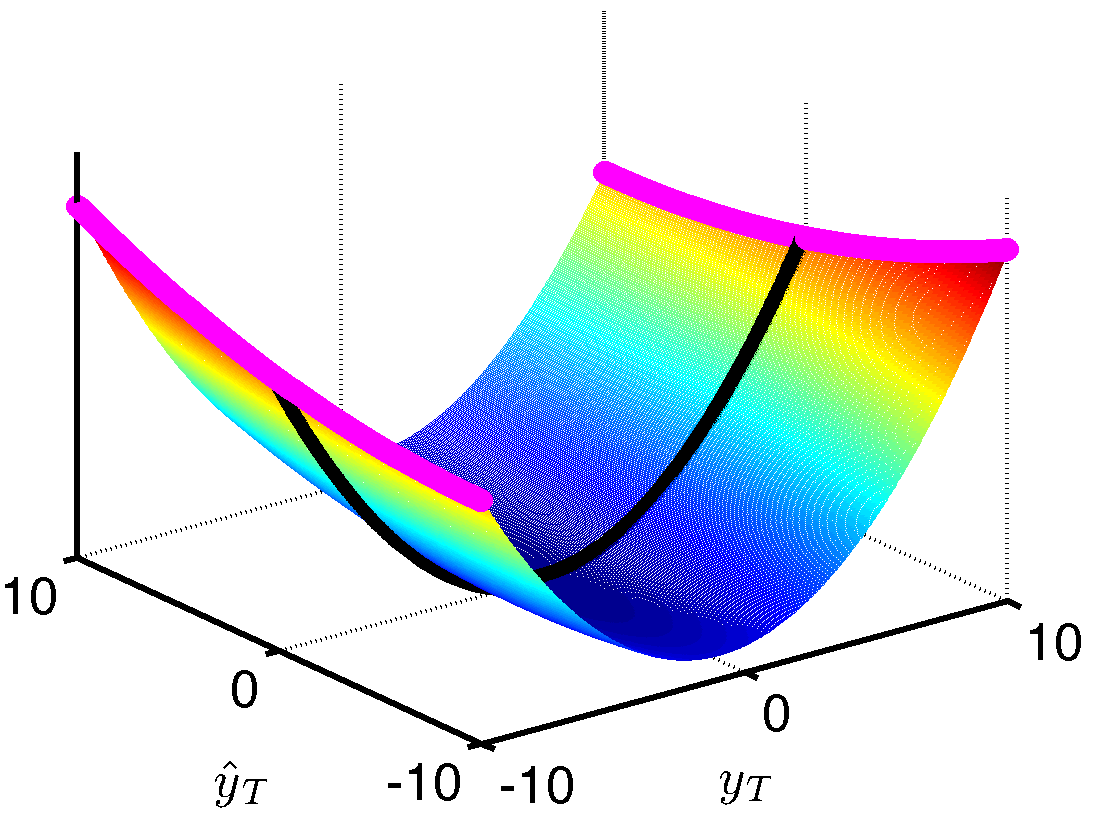
\includegraphics[width=0.32\textwidth]{figs/forster_minmax}
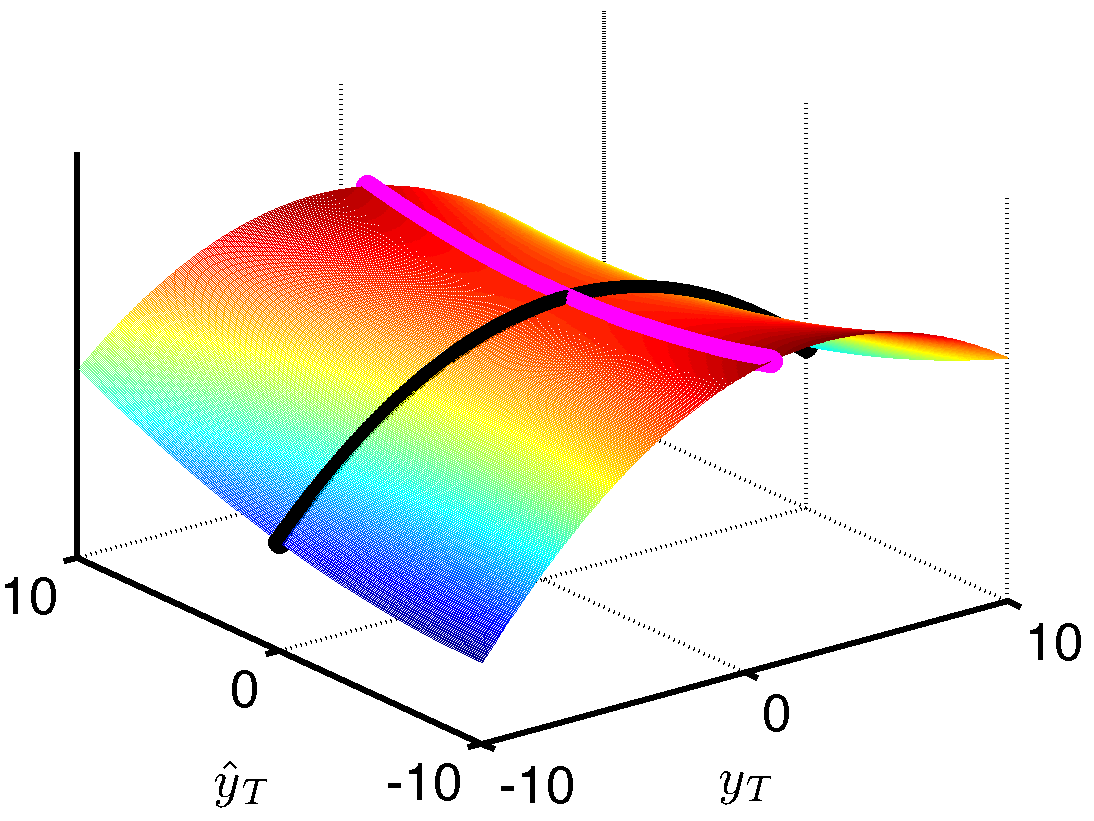
\includegraphics[width=0.32\textwidth]{figs/my_minmax}
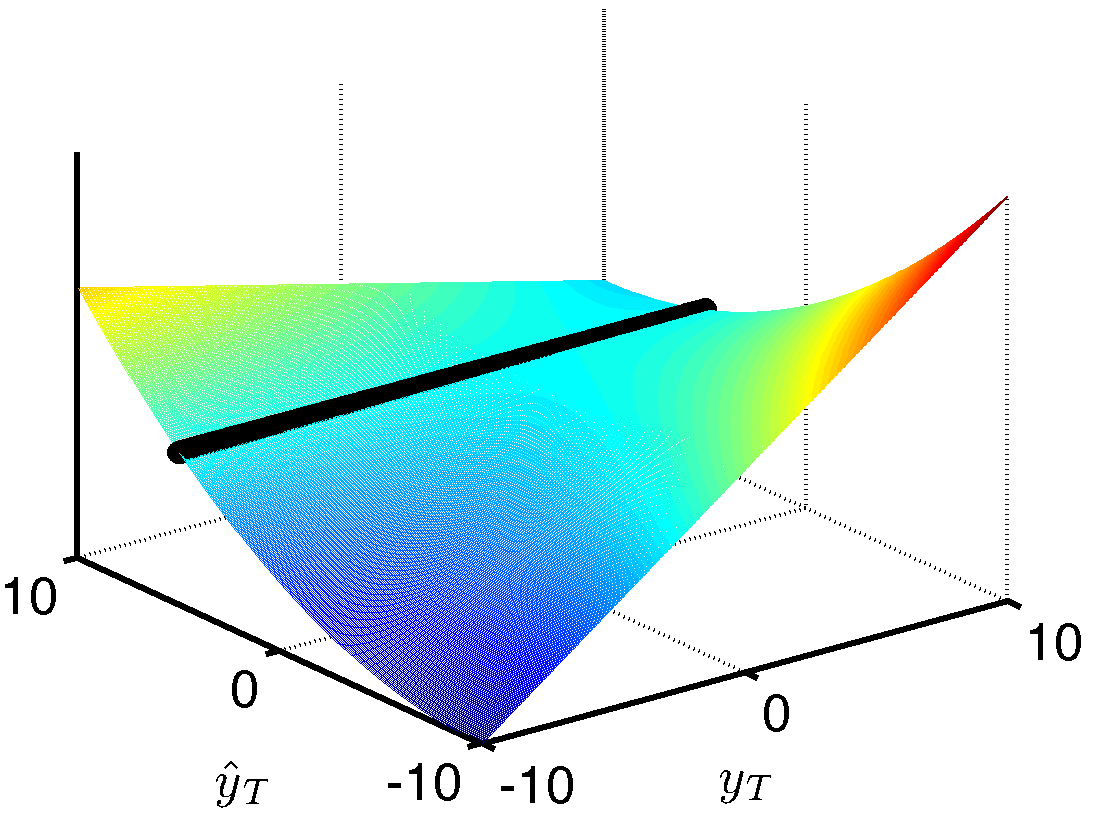
\includegraphics[width=0.32\textwidth]{figs/my_minmax_0}
\caption{
An illustration of the min-max objective function $G(\yi{T},\hyi{T})$
\eqref{minmax_objective}. The black line is the value of the objective
as a function of $\yi{T}$ for the optimal predictor $\hyi{T}$.
Left: Forster's optimization function (convex in $\yi{T}$).
Center: our optimization function (strictly  concave in $\yi{T}$,
case 1 in \thmref{thm:theorem1}).
Right: our optimization function (invariant to $\yi{T}$, case 2 in \thmref{thm:theorem1}).}
\label{fig:minmax}
\end{figure}
%

This phenomena is illustrated in the left panel
of \figref{fig:minmax} (best viewed in color).  For the min-max optimization function defined
by~\cite{Forster}, fixing some value of $\hat{y}_{T}$, the function
is convex in $y_{T}$, and the adversary would achieve a maximal value
at the boundary of the feasible values of $y_{T}$ interval. That is,
either $y_{T}=Y$ or $y_{T}=-Y$, as indicated by the two magenta lines
at $\yi{T}=\pm10$. The optimal predictor $\hat{y}_{T}$ is
achieved somewhere along the lines $y_{T}=Y$ or $y_{T}=-Y$.

% and showed that it is optimal when the last outcome variable is bounded,
% that is $y_{T}\in[-Y,Y]$. We next give similar result, but we do
% not assume that $y_{T}$ is bounded. Instead, other assumption is
% required.

% The difference between our and Forster optimization function is illustrated
% in the next figure:

We propose an alternative approach to make the min-max optimal solution
bounded by appropriately setting the weight $a_T$ such that
$G(\yi{T},\hyi{T})$ is concave in $\yi{T}$ for a constant
$\hat{y}_{T}$. We explicitly consider two cases.
%
First, set $a_T$ such that $G(\yi{T},\hyi{T})$ is {\em strictly
  concave} in $\yi{T}$, and thus attains a single maximum with no need
to artificially restrict the value of $\yi{T}$. The optimal predictor
$\hat{y}_{T}$ in this case is achieved in the unique saddle point, as illustrated
in the center panel of \figref{fig:minmax}.
%
A second case is to set $a_T$ such that $\alpha(a_T)=0$ and the
min-max function $G(\yi{T},\hyi{T})$ becomes linear in $\yi{T}$. Here,
the optimal prediction is achieved by choosing $\hyi{T}$ such that
$\beta(a_T, \hyi{T})=0$ which turns $G(\yi{T},\hyi{T})$ to be
invariant to $\yi{T}$, as illustrated in the right panel of
\figref{fig:minmax}.  % the for a
% specific choice of $\hat{y}_{T}$, because for other $\hat{y}_{T}$ the
% optimization function can made large by choosing $y_{T}$ with large
% absolute value.

Equipped with
\lemref{lem:lemma1} we develop the optimal solution of the min-max
predictor, summarized in the following theorem.
%
\begin{theorem}
\label{thm:theorem1}
Assume that $1+a_{T}\mathbf{x}_{T}^{\top}\mathbf{A}_{T-1}^{-1}\mathbf{x}_{T}-a_{T}\leq0$.
Then the optimal prediction for the last round $T$ is
\begin{align}
\hat{y}_{T}=\mathbf{b}_{T-1}^{\top}\mathbf{A}_{T-1}^{-1}\mathbf{x}_{T}
~. \label{laststep_minmax_optimal}
\end{align}
\end{theorem}
%
%The proof appears in \secref{proof_theorem1}
The proof of the theorem makes use of the following technical lemma.
\begin{lemma}
\label{lem:lemma2}
For all $t=1,2,\ldots,T$
\begin{equation}
a_{t}^{2}\mathbf{x}_{t}^{\top}\mathbf{A}_{t}^{-1}\mathbf{x}_{t}+1-a_{t}=\frac{1+a_{t}\mathbf{x}_{t}^{\top}\mathbf{A}_{t-1}^{-1}\mathbf{x}_{t}-a_{t}}{1+a_{t}\mathbf{x}_{t}^{\top}\mathbf{A}_{t-1}^{-1}\mathbf{x}_{t}}
~. \label{lemma2}
\end{equation}
\end{lemma}
\begin{proof}
Using the Woodbury identity we get
\[
\mathbf{A}_{t}^{-1}=\mathbf{A}_{t-1}^{-1}-\frac{\mathbf{A}_{t-1}^{-1}\mathbf{x}_{t}\mathbf{x}_{t}^{\top}\mathbf{A}_{t-1}^{-1}}{\frac{1}{a_{t}}+\mathbf{x}_{t}^{\top}\mathbf{A}_{t-1}^{-1}\mathbf{x}_{t}}~,
\]
 therefore the left side of \eqref{lemma2} is
\begin{eqnarray*}
a_{t}^{2}\mathbf{x}_{t}^{\top}\mathbf{A}_{t}^{-1}\mathbf{x}_{t}+1-a_{t}
 &=&  a_{t}^{2}\mathbf{x}_{t}^{\top}\left(\mathbf{A}_{t-1}^{-1}-\frac{\mathbf{A}_{t-1}^{-1}\mathbf{x}_{t}\mathbf{x}_{t}^{\top}\mathbf{A}_{t-1}^{-1}}{\frac{1}{a_{t}}+\mathbf{x}_{t}^{\top}\mathbf{A}_{t-1}^{-1}\mathbf{x}_{t}}\right)\mathbf{x}_{t}+1-a_{t}\\
  &=&  a_{t}^{2}\mathbf{x}_{t}^{\top}\mathbf{A}_{t-1}^{-1}\mathbf{x}_{t}-\frac{a_{t}^{2}\mathbf{x}_{t}^{\top}\mathbf{A}_{t-1}^{-1}\mathbf{x}_{t}\mathbf{x}_{t}^{\top}\mathbf{A}_{t-1}^{-1}\mathbf{x}_{t}}{\frac{1}{a_{t}}+\mathbf{x}_{t}^{\top}\mathbf{A}_{t-1}^{-1}\mathbf{x}_{t}}+1-a_{t}\\
  &=&  \frac{1+a_{t}\mathbf{x}_{t}^{\top}\mathbf{A}_{t-1}^{-1}\mathbf{x}_{t}-a_{t}}{1+a_{t}\mathbf{x}_{t}^{\top}\mathbf{A}_{t-1}^{-1}\mathbf{x}_{t}}~.
\end{eqnarray*}
\QED
 \end{proof}
We now prove \thmref{thm:theorem1}.
\begin{proof}
The adversary can choose any $y_{T}$, thus the algorithm should predict
$\hat{y}_{T}$ such that the following quantity is minimal,
\begin{eqnarray*}
&&\max_{y_{T}}\left(\sum_{t=1}^{T}\left(y_{t}-\hat{y}_{t}\right)^{2}-\inf_{\mathbf{u}\in\mathbb{R}^{d}}\left(b\left\Vert \mathbf{u}\right\Vert ^{2}+\sum_{t=1}^{T}a_{t}\left(y_{t}-\mathbf{u}^{\top}\mathbf{x}_{t}\right)^{2}\right)\right)\\
&\overset{\eqref{optimal_solution}}{=}&\max_{y_{T}}\left(\sum_{t=1}^{T}\left(y_{t}-\hat{y}_{t}\right)^{2}-\sum_{t=1}^{T}a_{t}y_{t}^{2}+\mathbf{b}_{T}^{\top}\mathbf{A}_{T}^{-1}\mathbf{b}_{T}\right) ~.
\end{eqnarray*}
That is, we need to solve the following min-max problem
\[
\min_{\hat{y}_{T}}\max_{y_{T}}\left(\sum_{t=1}^{T}\left(y_{t}-\hat{y}_{t}\right)^{2}-\sum_{t=1}^{T}a_{t}y_{t}^{2}+\mathbf{b}_{T}^{\top}\mathbf{A}_{T}^{-1}\mathbf{b}_{T}\right)~.
\]
We use the following relation to re-write the optimization problem,
\begin{align}
\mathbf{b}_{T}^{\top}\mathbf{A}_{T}^{-1}\mathbf{b}_{T}
%& = & \left(\mathbf{b}_{T-1}+a_{T}y_{T}\mathbf{x}_{T}\right)^{\top}\mathbf{A}_{T}^{-1}\left(\mathbf{b}_{T-1}+a_{T}y_{T}\mathbf{x}_{T}\right)\nonumber \\
 & = &
 \mathbf{b}_{T-1}^{\top}\mathbf{A}_{T}^{-1}\mathbf{b}_{T-1}+2a_{T}y_{T}\mathbf{b}_{T-1}^{\top}\mathbf{A}_{T}^{-1}\mathbf{x}_{T}+a_{T}^{2}y_{T}^{2}\mathbf{x}_{T}^{\top}\mathbf{A}_{T}^{-1}\mathbf{x}_{T} ~.\label{t3}
\end{align}
Omitting all terms that are
not depending on $y_{T}$ and $\hat{y}_{T}$,
\[
\min_{\hat{y}_{T}}\max_{y_{T}}\left(\left(y_{T}-\hat{y}_{T}\right)^{2}-a_{T}y_{T}^{2}+2a_{T}y_{T}\mathbf{b}_{T-1}^{\top}\mathbf{A}_{T}^{-1}\mathbf{x}_{T}+a_{T}^{2}y_{T}^{2}\mathbf{x}_{T}^{\top}\mathbf{A}_{T}^{-1}\mathbf{x}_{T}\right)~.
\]
We manipulate the last problem to be of form \eqref{minmax_objective} using \lemref{lem:lemma2},
% \[
% \min_{\hat{y}_{T}}\max_{y_{T}}\left(\left(a_{T}^{2}\mathbf{x}_{T}^{\top}\mathbf{A}_{T}^{-1}\mathbf{x}_{T}+1-a_{T}\right)y_{T}^{2}+2y_{T}\left(a_{T}\mathbf{b}_{T-1}^{\top}\mathbf{A}_{T}^{-1}\mathbf{x}_{T}-\hat{y}_{T}\right)+\hat{y}_{T}^{2}\right)
% \]
% and by lemma 2 we get
\begin{align}
\min_{\hat{y}_{T}}\max_{y_{T}} \left(\!
  \frac{1+a_{T}\mathbf{x}_{T}^{\top}\mathbf{A}_{T-1}^{-1}\mathbf{x}_{T}-a_{T}}{1+a_{T}\mathbf{x}_{T}^{\top}\mathbf{A}_{T-1}^{-1}\mathbf{x}_{T}}y_{T}^{2}+2y_{T}\left(a_{T}\mathbf{b}_{T-1}^{\top}\mathbf{A}_{T}^{-1}\mathbf{x}_{T}-\hat{y}_{T}\right)+\hat{y}_{T}^{2}
\!\right),\label{minmax}
\end{align}
where
\[
\alpha(a_T)=\frac{1+a_{T}\mathbf{x}_{T}^{\top}\mathbf{A}_{T-1}^{-1}\mathbf{x}_{T}-a_{T}}{1+a_{T}\mathbf{x}_{T}^{\top}\mathbf{A}_{T-1}^{-1}\mathbf{x}_{T}}
\quad\textrm{ and }\quad
\beta(a_T,\hyi{T})=a_{T}\mathbf{b}_{T-1}^{\top}\mathbf{A}_{T}^{-1}\mathbf{x}_{T}-\hat{y}_{T}~.
\]

We consider two cases:  (1)
$1+a_{T}\mathbf{x}_{T}^{\top}\mathbf{A}_{T-1}^{-1}\mathbf{x}_{T}-a_{T}<0$
(corresponding to the middle panel of \figref{fig:minmax}),
and (2)
$1+a_{T}\mathbf{x}_{T}^{\top}\mathbf{A}_{T-1}^{-1}\mathbf{x}_{T}-a_{T}=0$
(corresponding to the right panel of \figref{fig:minmax}),
starting with the first case,
\begin{equation}
1+a_{T}\mathbf{x}_{T}^{\top}\mathbf{A}_{T-1}^{-1}\mathbf{x}_{T}-a_{T}<0\label{option1}~.
\end{equation}
Denote the inner-maximization problem by,
\[
f\left(y_{T}\right)\!=\!\frac{1+a_{T}\mathbf{x}_{T}^{\top}\mathbf{A}_{T-1}^{-1}\mathbf{x}_{T}-a_{T}}{1+a_{T}\mathbf{x}_{T}^{\top}\mathbf{A}_{T-1}^{-1}\mathbf{x}_{T}}y_{T}^{2}+2y_{T}\left(a_{T}\mathbf{b}_{T-1}^{\top}\mathbf{A}_{T}^{-1}\mathbf{x}_{T}-\hat{y}_{T}\right)+\hat{y}_{T}^{2}~. 
\]
This function is strictly-concave with respect to $y_{T}$ because of
\eqref{option1}. Thus, it has a unique maximal value given by,
\begin{eqnarray*}
f^{max}(\hyi{T})
%& = & \hat{y}_{T}^{2}-\frac{\left(a_{T}\mathbf{b}_{T-1}^{\top}\mathbf{A}_{T}^{-1}\mathbf{x}_{T}-\hat{y}_{T}\right)^{2}\left(1+a_{T}\mathbf{x}_{T}^{\top}\mathbf{A}_{T-1}^{-1}\mathbf{x}_{T}\right)}{1+a_{T}\mathbf{x}_{T}^{\top}\mathbf{A}_{T-1}^{-1}\mathbf{x}_{T}-a_{T}}\\
 & = & -\frac{a_{T}}{1+a_{T}\mathbf{x}_{T}^{\top}\mathbf{A}_{T-1}^{-1}\mathbf{x}_{T}-a_{T}}\hat{y}_{T}^{2}+\frac{2a_{T}\mathbf{b}_{T-1}^{\top}\mathbf{A}_{T}^{-1}\mathbf{x}_{T}\left(1+a_{T}\mathbf{x}_{T}^{\top}\mathbf{A}_{T-1}^{-1}\mathbf{x}_{T}\right)}{1+a_{T}\mathbf{x}_{T}^{\top}\mathbf{A}_{T-1}^{-1}\mathbf{x}_{T}-a_{T}}\hat{y}_{T}\\
 &  & -\frac{\left(a_{T}\mathbf{b}_{T-1}^{\top}\mathbf{A}_{T}^{-1}\mathbf{x}_{T}\right)^{2}\left(1+a_{T}\mathbf{x}_{T}^{\top}\mathbf{A}_{T-1}^{-1}\mathbf{x}_{T}\right)}{1+a_{T}\mathbf{x}_{T}^{\top}\mathbf{A}_{T-1}^{-1}\mathbf{x}_{T}-a_{T}}~.
\end{eqnarray*}
Next, we solve $\min_{\hat{y}_{T}} f^{max}( \hyi{T} )$, which is strictly-convex
with respect to $\hat{y}_{T}$ because of \eqref{option1}. Solving this problem we get the optimal
last-step min-max predictor,
\begin{equation}
\hat{y}_{T}=\mathbf{b}_{T-1}^{\top}\mathbf{A}_{T}^{-1}\mathbf{x}_{T}\left(1+a_{T}\mathbf{x}_{T}^{\top}\mathbf{A}_{T-1}^{-1}\mathbf{x}_{T}\right)
~.
\label{t1}
\end{equation}
We further derive the last equation. From \eqref{Adef} we have,
\begin{equation}
\mathbf{A}_{T}^{-1}a_{T}\mathbf{x}_{T}\mathbf{x}_{T}^{\top}\mathbf{A}_{T-1}^{-1}=\mathbf{A}_{T}^{-1}\left(\mathbf{A}_{T}-\mathbf{A}_{T-1}\right)\mathbf{A}_{T-1}^{-1}=\mathbf{A}_{T-1}^{-1}-\mathbf{A}_{T}^{-1}\label{t2}~.
\end{equation}
Substituting \eqref{t2} in \eqref{t1} we have the following equality
as desired,
\begin{align}
\hat{y}_{T} & =  \mathbf{b}_{T-1}^{\top}\mathbf{A}_{T}^{-1}\mathbf{x}_{T}+\mathbf{b}_{T-1}^{\top}\mathbf{A}_{T}^{-1}a_{T}\mathbf{x}_{T}\mathbf{x}_{T}^{\top}\mathbf{A}_{T-1}^{-1}\mathbf{x}_{T}
 %& =  \mathbf{b}_{T-1}^{\top}\mathbf{A}_{T}^{-1}\mathbf{x}_{T}+\mathbf{b}_{T-1}^{\top}\left(\mathbf{A}_{T-1}^{-1}-\mathbf{A}_{T}^{-1}\right)\mathbf{x}_{T}\\
  =  \mathbf{b}_{T-1}^{\top}\mathbf{A}_{T-1}^{-1}\mathbf{x}_{T}~. \label{t3_thm}
\end{align}
%as desired.

We now move to the second case for which,
\(
1+a_{T}\mathbf{x}_{T}^{\top}\mathbf{A}_{T-1}^{-1}\mathbf{x}_{T}-a_{T}=0,
\)
which is written equivalently as,
\begin{equation}
a_{T}=\frac{1}{1-\mathbf{x}_{T}^{\top}\mathbf{A}_{T-1}^{-1}\mathbf{x}_{T}}
~. \label{aT}
\end{equation}
Substituting \eqref{aT} in \eqref{minmax} we get,
\[
\min_{\hat{y}_{T}}\max_{y_{T}}\left(2y_{T}\left(a_{T}\mathbf{b}_{T-1}^{\top}\mathbf{A}_{T}^{-1}\mathbf{x}_{T}-\hat{y}_{T}\right)+\hat{y}_{T}^{2}\right) ~.
\]
For $\hat{y}_{T}\neq
a_{T}\mathbf{b}_{T-1}^{\top}\mathbf{A}_{T}^{-1}\mathbf{x}_{T}$, the
value of the optimization problem is not-bounded as the adversary
may choose $\yi{T} =z^2
\left(a_{T}\mathbf{b}_{T-1}^{\top}\mathbf{A}_{T}^{-1}\mathbf{x}_{T}-\hat{y}_{T}\right)
$ for $z\rightarrow\infty$. Thus, the optimal last-step min-max prediction
is to set
$\hat{y}_{T}=a_{T}\mathbf{b}_{T-1}^{\top}\mathbf{A}_{T}^{-1}\mathbf{x}_{T}$.
Substituting $a_T =
1+a_{T}\mathbf{x}_{T}^{\top}\mathbf{A}_{T-1}^{-1}\mathbf{x}_{T}$ and
following the derivation from \eqref{t1} to \eqref{t3_thm} above, yields the
desired identity.
%
% To show that it is equal to
% $\mathbf{b}_{T-1}^{\top}\mathbf{A}_{T-1}^{-1}\mathbf{x}_{T}$ we use
% the Woodbury identity and get
% \begin{eqnarray*}
% \mathbf{A}_{T}^{-1} & = & \mathbf{A}_{T-1}^{-1}-\frac{\mathbf{A}_{T-1}^{-1}\mathbf{x}_{T}\mathbf{x}_{T}^{\top}\mathbf{A}_{T-1}^{-1}}{\frac{1}{a_{T}}+\mathbf{x}_{T}^{\top}\mathbf{A}_{T-1}^{-1}\mathbf{x}_{T}}\\
%  & \overset{\eqref{aT}}{=} & \mathbf{A}_{T-1}^{-1}-\frac{\mathbf{A}_{T-1}^{-1}\mathbf{x}_{T}\mathbf{x}_{T}^{\top}\mathbf{A}_{T-1}^{-1}}{1-\mathbf{x}_{T}^{\top}\mathbf{A}_{T-1}^{-1}\mathbf{x}_{T}+\mathbf{x}_{T}^{\top}\mathbf{A}_{T-1}^{-1}\mathbf{x}_{T}}\\
%  & = & \mathbf{A}_{T-1}^{-1}-\mathbf{A}_{T-1}^{-1}\mathbf{x}_{T}\mathbf{x}_{T}^{\top}\mathbf{A}_{T-1}^{-1}
% \end{eqnarray*}
%  therefore $\hat{y}_{T}$ can be written as
% \begin{eqnarray*}
% \hat{y}_{T} & = & a_{T}\mathbf{b}_{T-1}^{\top}\left(\mathbf{A}_{T-1}^{-1}-\mathbf{A}_{T-1}^{-1}\mathbf{x}_{T}\mathbf{x}_{T}^{\top}\mathbf{A}_{T-1}^{-1}\right)\mathbf{x}_{T}\\
%  & \overset{\eqref{aT}}{=} & \frac{1}{1-\mathbf{x}_{T}^{\top}\mathbf{A}_{T-1}^{-1}\mathbf{x}_{T}}\mathbf{b}_{T-1}^{\top}\mathbf{A}_{T-1}^{-1}\mathbf{x}_{T}\left(1-\mathbf{x}_{T}^{\top}\mathbf{A}_{T-1}^{-1}\mathbf{x}_{T}\right)\\
%  & = & \mathbf{b}_{T-1}^{\top}\mathbf{A}_{T-1}^{-1}\mathbf{x}_{T}
% \end{eqnarray*}
 \QED\end{proof}
% \begin{proof}
% Using the Woodbury matrix identity we get
% \begin{eqnarray}
% \mathbf{A}_{t}^{-1} & = & \mathbf{A}_{t-1}^{-1}-\frac{\mathbf{A}_{t-1}^{-1}\mathbf{x}_{t}\mathbf{x}_{t}^{\top}\mathbf{A}_{t-1}^{-1}}{\frac{1}{a_{t}}+\mathbf{x}_{t}^{\top}\mathbf{A}_{t-1}^{-1}\mathbf{x}_{t}}\label{woodbury}
% \end{eqnarray}
% therefore
% \begin{eqnarray}
% \mathbf{A}_{t}^{-1}\mathbf{x}_{t} & = & \mathbf{A}_{t-1}^{-1}\mathbf{x}_{t}-\frac{\mathbf{A}_{t-1}^{-1}\mathbf{x}_{t}\mathbf{x}_{t}^{\top}\mathbf{A}_{t-1}^{-1}\mathbf{x}_{t}}{\frac{1}{a_{t}}+\mathbf{x}_{t}^{\top}\mathbf{A}_{t-1}^{-1}\mathbf{x}_{t}}\nonumber \\
%  & = & \frac{\mathbf{A}_{t-1}^{-1}\mathbf{x}_{t}}{1+a_{t}\mathbf{x}_{t}^{\top}\mathbf{A}_{t-1}^{-1}\mathbf{x}_{t}}\label{t4}
% \end{eqnarray}
% For $1\leq t\leq T$ we have
% \begin{eqnarray*}
%  &  & \ell_{t}(\textrm{alg})+\min_{\mathbf{u}\in\mathbb{R}^{d}}\left(b\left\Vert \mathbf{u}\right\Vert ^{2}+L_{t-1}^{\boldsymbol{a}}(\mathbf{u})\right)-\min_{\mathbf{u}\in\mathbb{R}^{d}}\left(b\left\Vert \mathbf{u}\right\Vert ^{2}+L_{t}^{\boldsymbol{a}}(\mathbf{u})\right)\\
%  &  & =\left(y_{t}-\hat{y}_{t}\right)^{2}+\min_{\mathbf{u}\in\mathbb{R}^{d}}\left(b\left\Vert \mathbf{u}\right\Vert ^{2}+\sum_{s=1}^{t-1}a_{s}\left(y_{s}-\mathbf{u}^{\top}\mathbf{x}_{s}\right)^{2}\right)-\min_{\mathbf{u}\in\mathbb{R}^{d}}\left(b\left\Vert \mathbf{u}\right\Vert ^{2}+\sum_{s=1}^{t}a_{s}\left(y_{s}-\mathbf{u}^{\top}\mathbf{x}_{s}\right)^{2}\right)\\
%  &  & \overset{Lemma1}{=}\left(y_{t}-\hat{y}_{t}\right)^{2}+\sum_{s=1}^{t-1}a_{s}y_{s}^{2}-\mathbf{b}_{t-1}^{\top}\mathbf{A}_{t-1}^{-1}\mathbf{b}_{t-1}-\sum_{s=1}^{t}a_{s}y_{s}^{2}+\mathbf{b}_{t}^{\top}\mathbf{A}_{t}^{-1}\mathbf{b}_{t}\\
%  &  & =\left(y_{t}-\hat{y}_{t}\right)^{2}-a_{t}y_{t}^{2}-\mathbf{b}_{t-1}^{\top}\mathbf{A}_{t-1}^{-1}\mathbf{b}_{t-1}+\mathbf{b}_{t}^{\top}\mathbf{A}_{t}^{-1}\mathbf{b}_{t}\\
%  &  & \overset{\eqref{t3}}{=}\left(y_{t}-\hat{y}_{t}\right)^{2}-a_{t}y_{t}^{2}-\mathbf{b}_{t-1}^{\top}\mathbf{A}_{t-1}^{-1}\mathbf{b}_{t-1}+\mathbf{b}_{t-1}^{\top}\mathbf{A}_{t}^{-1}\mathbf{b}_{t-1}+2a_{t}y_{t}\mathbf{b}_{t-1}^{\top}\mathbf{A}_{t}^{-1}\mathbf{x}_{t}+a_{t}^{2}y_{t}^{2}\mathbf{x}_{t}^{\top}\mathbf{A}_{t}^{-1}\mathbf{x}_{t}\\
%  &  & =\left(y_{t}-\hat{y}_{t}\right)^{2}-a_{t}y_{t}^{2}-\mathbf{b}_{t-1}^{\top}\left(\mathbf{A}_{t-1}^{-1}-\mathbf{A}_{t}^{-1}\right)\mathbf{b}_{t-1}+2a_{t}y_{t}\mathbf{b}_{t-1}^{\top}\mathbf{A}_{t}^{-1}\mathbf{x}_{t}+a_{t}^{2}y_{t}^{2}\mathbf{x}_{t}^{\top}\mathbf{A}_{t}^{-1}\mathbf{x}_{t}\\
%  &  & \overset{\eqref{t2}}{=}\left(y_{t}-\hat{y}_{t}\right)^{2}-a_{t}y_{t}^{2}-\mathbf{b}_{t-1}^{\top}\mathbf{A}_{t}^{-1}a_{t}\mathbf{x}_{t}\mathbf{x}_{t}^{\top}\mathbf{A}_{t-1}^{-1}\mathbf{b}_{t-1}+2a_{t}y_{t}\mathbf{b}_{t-1}^{\top}\mathbf{A}_{t}^{-1}\mathbf{x}_{t}+a_{t}^{2}y_{t}^{2}\mathbf{x}_{t}^{\top}\mathbf{A}_{t}^{-1}\mathbf{x}_{t}\\
%  &  & =\left(y_{t}-\hat{y}_{t}\right)^{2}-a_{t}y_{t}^{2}+a_{t}\left(-\hat{y}_{t}\mathbf{b}_{t-1}^{\top}+2y_{t}\mathbf{b}_{t-1}^{\top}+a_{t}y_{t}^{2}\mathbf{x}_{t}^{\top}\right)\mathbf{A}_{t}^{-1}\mathbf{x}_{t}\\
%  &  & \overset{\eqref{t4}}{=}\left(y_{t}-\hat{y}_{t}\right)^{2}-a_{t}y_{t}^{2}+a_{t}\left(-\hat{y}_{t}\mathbf{b}_{t-1}^{\top}+2y_{t}\mathbf{b}_{t-1}^{\top}+a_{t}y_{t}^{2}\mathbf{x}_{t}^{\top}\right)\frac{\mathbf{A}_{t-1}^{-1}\mathbf{x}_{t}}{1+a_{t}\mathbf{x}_{t}^{\top}\mathbf{A}_{t-1}^{-1}\mathbf{x}_{t}}\\
%  &  & =\left(y_{t}-\hat{y}_{t}\right)^{2}+a_{t}\frac{-y_{t}^{2}-y_{t}^{2}a_{t}\mathbf{x}_{t}^{\top}\mathbf{A}_{t-1}^{-1}\mathbf{x}_{t}-\hat{y}_{t}^{2}+2y_{t}\hat{y}_{t}+a_{t}y_{t}^{2}\mathbf{x}_{t}^{\top}\mathbf{A}_{t-1}^{-1}\mathbf{x}_{t}}{1+a_{t}\mathbf{x}_{t}^{\top}\mathbf{A}_{t-1}^{-1}\mathbf{x}_{t}}\\
%  &  & =\left(y_{t}-\hat{y}_{t}\right)^{2}-a_{t}\frac{\left(y_{t}-\hat{y}_{t}\right)^{2}}{1+a_{t}\mathbf{x}_{t}^{\top}\mathbf{A}_{t-1}^{-1}\mathbf{x}_{t}}\\
%  &  & =\frac{1+a_{t}\mathbf{x}_{t}^{\top}\mathbf{A}_{t-1}^{-1}\mathbf{x}_{t}-a_{t}}{1+a_{t}\mathbf{x}_{t}^{\top}\mathbf{A}_{t-1}^{-1}\mathbf{x}_{t}}\left(y_{t}-\hat{y}_{t}\right)^{2}\leq0
% \end{eqnarray*}
% Summing over $t\in\left\{ 1,\ldots,T\right\} $ we get, %and using \eqref{LT}
% gives
% \[
% L_{T}(\textrm{alg})-\min_{\mathbf{u}\in\mathbb{R}^{d}}\left(b\left\Vert \mathbf{u}\right\Vert ^{2}+L_{T}^{\boldsymbol{a}}(\mathbf{u})\right)\leq0
% \]
 %
% \QED\end{proof}
 %
% \subsection{consume here}
%
% Our algorithm
%
% For our first algorithm we propose a variant of this algorithm which
% solves the following prpblem
%
% In\cite{Forster}, Forster proposed the following predictor for the last
% round
% \[
% \hat{y}_{T}=clip\left(\mathbf{b}_{T-1}^{\top}\mathbf{A}_{T}^{-1}\mathbf{x}_{T},Y\right)
% \]
% and showed that it is optimal when the last outcome variable is bounded,
% that is $y_{T}\in[-Y,Y]$. We next give similar result, but we do
% not assume that $y_{T}$ is bounded. Instead, other assumption is
% required.
%
% \cite{Forster} solved a variant of this problem, yet because the
% problem is convex in $\yi{T}$ kkk
%
% predicts a
% $\paren{\vxti{t}\vwi{t-1}-\yi{t}}^2$
% We will show below that a
% min-max algorithm also chooses a linear function, that is we have,
% $\hyi{t} = \vxti{t}\vwi{t-1}$ for some $\vwi{t-1}\in\reals^d$.

% We will also use an extended notion of evaluation, comparing
% our algorithm to a sequence of functions,
%
%  where there is some restriction over the sequence
%  ${\vui{1}\comdots\vui{T}}$.
%
% This generalization will help us to get results for more complex scenarios,
% such as non-stationary models.
%
%
% In this section we calculate the best prediction for Learner in the
% last round and we prove an upper bound on the regret for linear regression
% with square loss. Unlike\cite{Forster}, we do not assume here that the outcome
% variable is bounded.
%
% Like in\cite{Forster}, we consider the following protocol of interaction
% between Learner and adversary: \\
% FOR $t=1,2,3,\ldots,T$
% \begin{itemize}
% \item adversary chooses an instance $\mathbf{x}_{t}\in\mathbb{R}^{d}$
% \item learner chooses a prediction $\hat{y}_{t}\in\mathbb{R}$
% \item adversary chooses an outcome $y_{t}\in\mathbb{R}$
% \end{itemize}
% END FOR
%
% \noindent \begin{flushleft}
% At each round $t$ the loss of the learner is
% \par\end{flushleft}
%
% \noindent \begin{flushleft}
% \[
% \ell_{t}(\textrm{alg})=\left(y_{t}-\hat{y}_{t}\right)^{2}
% \]
% and after $T$ rounds, the total loss of the learner is
% \par\end{flushleft}
%
% \begin{equation}
% L_{T}(\textrm{alg})=\sum_{t=1}^{T}\ell_{t}(\textrm{alg})\label{LT}
% \end{equation}
%

We conclude by noting that although we did not restrict the form of
the predictor $\hyi{T}$, it turns out that it is a linear predictor
defined by $\hyi{T} = \vxti{T}\vwi{T-1}$ for $\vwi{T-1} =
\mathbf{A}_{T-1}^{-1}\mathbf{b}_{T-1}$. In other words, the functional
form of the optimal predictor is the same as the form of the
comparison function class - linear functions in our case. We call the
algorithm (defined using \eqref{Adef}, \eqref{bdef} and
\eqref{laststep_minmax_optimal}) \texttt{WEMM} for weighted min-max
prediction, and it is summarised in \figref{algorithm:WEMM}.
We note that \texttt{WEMM}
can also be seen as an incremental off-line
algorithm~\citep{AzouryWa01} or follow-the-leader, on a
weighted sequence: The prediction $\hyi{T} =
\vxti{T}\vwi{T-1}$ is with a model that is optimal over a prefix of length $T-1$.  The prediction of the optimal
predictor defined in \eqref{optimal_solution} is
$\vxti{T}\mathbf{u}_{T-1}=\vxti{T}\mathbf{A}_{T-1}^{-1}\mathbf{b}_{T-1}=\hat{y}_T$,
where $\hat{y}_T$ was defined in \eqref{laststep_minmax_optimal}.

\begin{figure}[t]
{
\paragraph{Parameter:} $1<b$
\paragraph{Initialize:} Set
$\mathbf{A}_{0}=b\,\mathbf{I}\in\reals^{d\times d}$ and
$\mathbf{b}_0=\vzero\in\reals^d$\\
{\bf For $t=1 \comdots T$} do
\begin{itemize}
\nolineskips
\item Receive an instance $\vxi{t}$
\item Output  prediction $\hyi{t}=\mathbf{b}_{t-1}^{\top}\mathbf{A}_{t-1}^{-1}\mathbf{x}_{t}$
\item Receive the correct label $\yi{t}$
\item
Set weight:
\begin{align*}
a_{t}&=\frac{1}{1-\mathbf{x}_{t}^{\top}\mathbf{A}_{t-1}^{-1}\mathbf{x}_{t}}
\end{align*}
\item
Update:
\begin{align*}
\mathbf{A}_{t}&=\mathbf{A}_{t-1}+a_{t}\mathbf{x}_{t}\mathbf{x}_{t}^{\top}
\\
\mathbf{b}_{t}&=\mathbf{b}_{t-1}+a_{t}\yi{t}\mathbf{x}_{t}
\end{align*}
\end{itemize}
\paragraph{Output:}  $\mathbf{A}_{T} \ ,\ \mathbf{b}_{T}$\\
}
\figline
\caption{WEMM: weighted min-max prediction.}
\label{algorithm:WEMM}
\end{figure}


\section{Recursive form}
\label{sec:WEMM_recursive}

Although \thmref{thm:theorem1} is correct for
$1+a_{T}\mathbf{x}_{T}^{\top}\mathbf{A}_{T-1}^{-1}\mathbf{x}_{T}-a_{T}\leq0$,
for the rest of the work we will assume an equality, that is
\begin{align}
a_{t}=\frac{1}{1-\mathbf{x}_{t}^{\top}\mathbf{A}_{t-1}^{-1}\mathbf{x}_{t}} \quad,\quad t=1 \dots T~.
\label{aa_t}
\end{align}
For this case, the \texttt{WEMM} algorithm can be expressed in a recursive form in terms of weight vector $\mathbf{w}_{t}$ and a covariance-like matrix $\mathbf{\Sigma}_{t}$. We denote $\mathbf{w}_{t}=\mathbf{A}_{t}^{-1}\mathbf{b}_{t}$ and $\mathbf{\Sigma}_{t}=\mathbf{A}_{t}^{-1}$, and develop recursive update rules for $\mathbf{w}_{t}$ and $\mathbf{\Sigma}_{t}$:
\begin{eqnarray}
\mathbf{w}_{t} & = & \mathbf{A}_{t}^{-1}\mathbf{b}_{t} \nonumber \\
 & = & \left(\mathbf{A}_{t-1}+a_{t}\mathbf{x}_{t}\mathbf{x}_{t}^{\top}\right)^{-1}\left(\mathbf{b}_{t-1}+a_{t}y_{t}\mathbf{x}_{t}\right) \nonumber \\
 & = & \left(\mathbf{A}_{t-1}^{-1}-\frac{\mathbf{A}_{t-1}^{-1}\mathbf{x}_{t}\mathbf{x}_{t}^{\top}\mathbf{A}_{t-1}^{-1}}{a_{t}^{-1}+\mathbf{x}_{t}^{\top}\mathbf{A}_{t-1}^{-1}\mathbf{x}_{t}}\right)\left(\mathbf{b}_{t-1}+a_{t}y_{t}\mathbf{x}_{t}\right) \nonumber \\
 & = & \mathbf{w}_{t-1}-\frac{\mathbf{A}_{t-1}^{-1}\mathbf{x}_{t}\mathbf{x}_{t}^{\top}\mathbf{w}_{t-1}}{a_{t}^{-1}+\mathbf{x}_{t}^{\top}\mathbf{A}_{t-1}^{-1}\mathbf{x}_{t}}+a_{t}y_{t}\mathbf{A}_{t-1}^{-1}\mathbf{x}_{t}-\frac{a_{t}y_{t}\mathbf{A}_{t-1}^{-1}\mathbf{x}_{t}\mathbf{x}_{t}^{\top}\mathbf{A}_{t-1}^{-1}\mathbf{x}_{t}}{a_{t}^{-1}+\mathbf{x}_{t}^{\top}\mathbf{A}_{t-1}^{-1}\mathbf{x}_{t}} \nonumber \\
 & = & \mathbf{w}_{t-1}+\frac{y_{t}\mathbf{A}_{t-1}^{-1}\mathbf{x}_{t}-\mathbf{A}_{t-1}^{-1}\mathbf{x}_{t}\mathbf{x}_{t}^{\top}\mathbf{w}_{t-1}}{a_{t}^{-1}+\mathbf{x}_{t}^{\top}\mathbf{A}_{t-1}^{-1}\mathbf{x}_{t}} \nonumber \\
 & \overset{\eqref{aa_t}}{=} & \mathbf{w}_{t-1}+\left(y_{t}-\mathbf{x}_{t}^{\top}\mathbf{w}_{t-1}\right)\mathbf{A}_{t-1}^{-1}\mathbf{x}_{t} \nonumber \\
 & = & \mathbf{w}_{t-1}+\left(y_{t}-\mathbf{x}_{t}^{\top}\mathbf{w}_{t-1}\right)\mathbf{\Sigma}_{t-1}\mathbf{x}_{t}~, \label{w_t}
\end{eqnarray}
and
\begin{eqnarray*}
\mathbf{\Sigma}_{t}^{-1} & = & \mathbf{A}_{t}=\mathbf{A}_{t-1}+a_{t}\mathbf{x}_{t}\mathbf{x}_{t}^{\top}  \\
 & \overset{\eqref{aa_t}}{=} & \mathbf{A}_{t-1}+\frac{\mathbf{x}_{t}\mathbf{x}_{t}^{\top}}{1-\mathbf{x}_{t}^{\top}\mathbf{A}_{t-1}^{-1}\mathbf{x}_{t}} \\
 & = & \mathbf{\Sigma}_{t-1}^{-1}+\frac{\mathbf{x}_{t}\mathbf{x}_{t}^{\top}}{1-\mathbf{x}_{t}^{\top}\mathbf{\Sigma}_{t-1}\mathbf{x}_{t}} \end{eqnarray*}
or
\begin{eqnarray}
\mathbf{\Sigma}_{t} & = & \mathbf{\Sigma}_{t-1}-\mathbf{\Sigma}_{t-1}\mathbf{x}_{t}\mathbf{x}_{t}^{\top}\mathbf{\Sigma}_{t-1}~. \label{sigma_t}
\end{eqnarray}
A summary of the algorithm in a recursive form appears in the right column of \tabref{table:algorithms}.

%\begin{figure}[t!]
%{
%\paragraph{Parameter:} $1<b$
%\paragraph{Initialize:} Set
%$\mathbf{w}_0=\vzero\in\reals^d$ and
%$\mathbf{\Sigma}_{0}=b^{-1}\,\mathbf{I}\in\reals^{d\times d}$\\
%{\bf For $t=1 \comdots T$} do
%\begin{itemize}
%\nolineskips
%\item Receive an instance $\vxi{t}$
%\item Output  prediction $\hyi{t}=\mathbf{x}_{t}^{\top}\mathbf{w}_{t-1}$
%\item Receive the correct label $\yi{t}$
%\item
%Update:
%\begin{align}
%\mathbf{w}_{t}&=\mathbf{w}_{t-1}+\left(y_{t}-\mathbf{x}_{t}^{\top}\mathbf{w}_{t-1}\right)\mathbf{\Sigma}_{t-1}\mathbf{x}_{t}
%\label{w_t}\\
%\mathbf{\Sigma}_{t}&=\mathbf{\Sigma}_{t-1}-\mathbf{\Sigma}_{t-1}\mathbf{x}_{t}\mathbf{x}_{t}^{\top}\mathbf{\Sigma}_{t-1}
%\label{sigma_t}
%\end{align}
%\end{itemize}
%\paragraph{Output:}  $\mathbf{w}_{T} \ ,\ \mathbf{\Sigma}_{T}$\\
%}
%\figline
%\caption{WEMM: weighted min-max prediction.}
%\label{algorithm:WEMM}
%\end{figure}

\section{Kernel version of the algorithm}
\label{sec:WEMM_kernel}

In this section we show that the \texttt{WEMM} algorithm can be expressed in dual variables, which allows an efficient run of the algorithm in any reproducing kernel Hilbert space.
%
We show by induction that the weight-vector $\mathbf{w}_{t}$ and
the covariance matrix $\mathbf{\Sigma}_{t}$ computed by the \texttt{WEMM}
algorithm in the right column of \tabref{table:algorithms} can be written in the form
\begin{eqnarray*}
\mathbf{w}_{t} & = & \sum_{i=1}^{t}\alpha_{i}^{\left(t\right)}\mathbf{x}_{i}\\
\mathbf{\Sigma}_{t} & = & \sum_{j=1}^{t}\sum_{k=1}^{t}\beta_{j,k}^{\left(t\right)}\mathbf{x}_{j}\mathbf{x}_{k}^{\top}+b^{-1}\mathbf{I}~,
\end{eqnarray*}
 where the coefficients $\alpha_{i}$ and $\beta_{j,k}$ depend only
on inner products of the input vectors.

For the initial step we have $\mathbf{w}_{0}=\mathbf{0}$ and $\mathbf{\Sigma}_{0}=b^{-1}\mathbf{I}$
which are trivially written in the desired form by setting $\alpha^{\left(0\right)}=0$
and $\beta^{\left(0\right)}=0$. We proceed to the induction step.
From the weight-vector update rule \eqref{w_t} we get
\begin{eqnarray*}
\mathbf{w}_{t} & = & \mathbf{w}_{t-1}+\left(y_{t}-\mathbf{x}_{t}^{\top}\mathbf{w}_{t-1}\right)\mathbf{\Sigma}_{t-1}\mathbf{x}_{t}=\\
 & = & \sum_{i=1}^{t-1}\alpha_{i}^{\left(t-1\right)}\mathbf{x}_{i}+\left(y_{t}-\mathbf{x}_{t}^{\top}\sum_{i=1}^{t-1}\alpha_{i}^{\left(t-1\right)}\mathbf{x}_{i}\right)\left(\sum_{j=1}^{t-1}\sum_{k=1}^{t-1}\beta_{j,k}^{\left(t-1\right)}\mathbf{x}_{j}\mathbf{x}_{k}^{\top}+b^{-1}\mathbf{I}\right)\mathbf{x}_{t}\\
 & = & \sum_{i=1}^{t-1}\alpha_{i}^{\left(t-1\right)}\mathbf{x}_{i}+\left(y_{t}-\sum_{i=1}^{t-1}\alpha_{i}^{\left(t-1\right)}\left(\mathbf{x}_{t}^{\top}\mathbf{x}_{i}\right)\right)\left(\sum_{j=1}^{t-1}\sum_{k=1}^{t-1}\beta_{j,k}^{\left(t-1\right)}\left(\mathbf{x}_{k}^{\top}\mathbf{x}_{t}\right)\mathbf{x}_{j}+b^{-1}\mathbf{x}_{t}\right)\\
 & = & \sum_{i=1}^{t-1}\left[\alpha_{i}^{\left(t-1\right)}+\left(y_{t}-\sum_{l=1}^{t-1}\alpha_{l}^{\left(t-1\right)}\left(\mathbf{x}_{t}^{\top}\mathbf{x}_{l}\right)\right)\sum_{k=1}^{t-1}\beta_{i,k}^{\left(t-1\right)}\left(\mathbf{x}_{k}^{\top}\mathbf{x}_{t}\right)\right]\mathbf{x}_{i}\\
 &&+b^{-1}\left(y_{t}-\sum_{i=1}^{t-1}\alpha_{i}^{\left(t-1\right)}\left(\mathbf{x}_{t}^{\top}\mathbf{x}_{i}\right)\right)\mathbf{x}_{t}~,
\end{eqnarray*}
 thus
\[
\alpha_{i}^{\left(t\right)}=\begin{cases}
\alpha_{i}^{\left(t-1\right)}+\left(y_{t}-\sum_{l=1}^{t-1}\alpha_{l}^{\left(t-1\right)}\left(\mathbf{x}_{t}^{\top}\mathbf{x}_{l}\right)\right)\sum_{k=1}^{t-1}\beta_{i,k}^{\left(t-1\right)}\left(\mathbf{x}_{k}^{\top}\mathbf{x}_{t}\right) & ~~ i=1 \comdots t-1\\
b^{-1}\left(y_{t}-\sum_{l=1}^{t-1}\alpha_{l}^{\left(t-1\right)}\left(\mathbf{x}_{t}^{\top}\mathbf{x}_{l}\right)\right) & ~~ i=t
\end{cases}
\]
From the covariance matrix update rule \eqref{sigma_t} we get
\begin{eqnarray*}
\mathbf{\Sigma}_{t} & = & \mathbf{\Sigma}_{t-1}-\mathbf{\Sigma}_{t-1}\mathbf{x}_{t}\mathbf{x}_{t}^{\top}\mathbf{\Sigma}_{t-1}\\
 & = & \sum_{j=1}^{t-1}\sum_{k=1}^{t-1}\beta_{j,k}^{\left(t-1\right)}\mathbf{x}_{j}\mathbf{x}_{k}^{\top}+b^{-1}\mathbf{I}\\
 &&-\left(\sum_{j=1}^{t-1}\sum_{k=1}^{t-1}\beta_{j,k}^{\left(t-1\right)}\mathbf{x}_{j}\mathbf{x}_{k}^{\top}+b^{-1}\mathbf{I}\right)\mathbf{x}_{t}\mathbf{x}_{t}^{\top}\left(\sum_{j=1}^{t-1}\sum_{k=1}^{t-1}\beta_{j,k}^{\left(t-1\right)}\mathbf{x}_{j}\mathbf{x}_{k}^{\top}+b^{-1}\mathbf{I}\right)\\
 & = & \sum_{j=1}^{t-1}\sum_{k=1}^{t-1}\beta_{j,k}^{\left(t-1\right)}\mathbf{x}_{j}\mathbf{x}_{k}^{\top}+b^{-1}\mathbf{I}\\
 &&-\left(\sum_{j=1}^{t-1}\sum_{k=1}^{t-1}\beta_{j,k}^{\left(t-1\right)}\left(\mathbf{x}_{k}^{\top}\mathbf{x}_{t}\right)\mathbf{x}_{j}+b^{-1}\mathbf{x}_{t}\right)\left(\sum_{j=1}^{t-1}\sum_{k=1}^{t-1}\beta_{j,k}^{\left(t-1\right)}\left(\mathbf{x}_{t}^{\top}\mathbf{x}_{j}\right)\mathbf{x}_{k}^{\top}+b^{-1}\mathbf{x}_{t}^{\top}\right)\\
 & = & \sum_{j=1}^{t-1}\sum_{k=1}^{t-1}\beta_{j,k}^{\left(t-1\right)}\mathbf{x}_{j}\mathbf{x}_{k}^{\top}+b^{-1}\mathbf{I}-\sum_{j=1}^{t-1}\sum_{k=1}^{t-1}\sum_{l=1}^{t-1}\sum_{m=1}^{t-1}\beta_{l,m}^{\left(t-1\right)}\beta_{j,k}^{\left(t-1\right)}\left(\mathbf{x}_{k}^{\top}\mathbf{x}_{t}\right)\left(\mathbf{x}_{t}^{\top}\mathbf{x}_{l}\right)\mathbf{x}_{j}\mathbf{x}_{m}^{\top}\\
 &  & -b^{-1}\sum_{j=1}^{t-1}\sum_{k=1}^{t-1}\beta_{j,k}^{\left(t-1\right)}\left(\mathbf{x}_{t}^{\top}\mathbf{x}_{j}\right)\mathbf{x}_{t}\mathbf{x}_{k}^{\top}-b^{-1}\sum_{j=1}^{t-1}\sum_{k=1}^{t-1}\beta_{j,k}^{\left(t-1\right)}\left(\mathbf{x}_{k}^{\top}\mathbf{x}_{t}\right)\mathbf{x}_{j}\mathbf{x}_{t}^{\top}-b^{-2}\mathbf{x}_{t}\mathbf{x}_{t}^{\top}\\
 & = & \sum_{j=1}^{t-1}\sum_{k=1}^{t-1}\left[\beta_{j,k}^{\left(t-1\right)}-\sum_{l=1}^{t-1}\sum_{m=1}^{t-1}\beta_{l,k}^{\left(t-1\right)}\beta_{j,m}^{\left(t-1\right)}\left(\mathbf{x}_{m}^{\top}\mathbf{x}_{t}\right)\left(\mathbf{x}_{t}^{\top}\mathbf{x}_{l}\right)\right]\mathbf{x}_{j}\mathbf{x}_{k}^{\top}+b^{-1}\mathbf{I}\\
 &  & -b^{-1}\sum_{k=1}^{t-1}\sum_{j=1}^{t-1}\beta_{j,k}^{\left(t-1\right)}\left(\mathbf{x}_{t}^{\top}\mathbf{x}_{j}\right)\mathbf{x}_{t}\mathbf{x}_{k}^{\top}-b^{-1}\sum_{j=1}^{t-1}\sum_{k=1}^{t-1}\beta_{j,k}^{\left(t-1\right)}\left(\mathbf{x}_{k}^{\top}\mathbf{x}_{t}\right)\mathbf{x}_{j}\mathbf{x}_{t}^{\top}-b^{-2}\mathbf{x}_{t}\mathbf{x}_{t}^{\top}~,
\end{eqnarray*}
 thus
\[
\beta_{j,k}^{\left(t\right)}=\begin{cases}
\beta_{j,k}^{\left(t-1\right)}-\sum_{l=1}^{t-1}\sum_{m=1}^{t-1}\beta_{l,k}^{\left(t-1\right)}\beta_{j,m}^{\left(t-1\right)}\left(\mathbf{x}_{m}^{\top}\mathbf{x}_{t}\right)\left(\mathbf{x}_{t}^{\top}\mathbf{x}_{l}\right) & ~~ j,k=1 \comdots t-1\\
-b^{-1}\sum_{l=1}^{t-1}\beta_{l,k}^{\left(t-1\right)}\left(\mathbf{x}_{t}^{\top}\mathbf{x}_{l}\right) & ~~ j=t~,~k=1 \comdots t-1\\
-b^{-1}\sum_{l=1}^{t-1}\beta_{j,l}^{\left(t-1\right)}\left(\mathbf{x}_{l}^{\top}\mathbf{x}_{t}\right) & ~~  k=t~,~j=1 \comdots t-1\\
-b^{-2} & ~~ j=k=t
\end{cases}
\]
 A summary of the kernel version of the \texttt{WEMM} algorithm appears in \figref{algorithm:kernel_WEMM}.

\begin{figure}[t!]
{
\paragraph{Parameter:} $1<b$, kernel function $K:\mathbb{R}^{d}\times\mathbb{R}^{d}\rightarrow\mathbb{R}$
\paragraph{Initialize:} Set
$\alpha^{\left(0\right)}=0$ and $\beta^{\left(0\right)}=0$\\
{\bf For $t=1 \comdots T$} do
\begin{itemize}
\nolineskips
\item Receive an instance $\vxi{t}$
\item Output  prediction $\hyi{t}=\sum_{i=1}^{t-1}\alpha_{i}^{\left(t-1\right)}K\left(\mathbf{x}_{t},\mathbf{x}_{i}\right)$
\item Receive the correct label $\yi{t}$
\item
Update:
\begin{align*}
\alpha_{i}^{\left(t\right)}&=\begin{cases}
\alpha_{i}^{\left(t-1\right)}+\left(y_{t}-\sum_{l=1}^{t-1}\alpha_{l}^{\left(t-1\right)}K\left(\mathbf{x}_{t},\mathbf{x}_{l}\right)\right)\sum_{k=1}^{t-1}\beta_{i,k}^{\left(t-1\right)}K\left(\mathbf{x}_{k},\mathbf{x}_{t}\right)
& ~~ i=1 \comdots t-1\\
b^{-1}\left(y_{t}-\sum_{l=1}^{t-1}\alpha_{l}^{\left(t-1\right)}K\left(\mathbf{x}_{t},\mathbf{x}_{l}\right)\right) & ~~ i=t
\end{cases}\\
\beta_{j,k}^{\left(t\right)}&=\begin{cases}
\beta_{j,k}^{\left(t-1\right)}-\sum_{l=1}^{t-1}\sum_{m=1}^{t-1}\beta_{l,k}^{\left(t-1\right)}\beta_{j,m}^{\left(t-1\right)}K\left(\mathbf{x}_{m},\mathbf{x}_{t}\right)K\left(\mathbf{x}_{t},\mathbf{x}_{l}\right)
& ~~ j,k=1 \comdots t-1\\
-b^{-1}\sum_{l=1}^{t-1}\beta_{l,k}^{\left(t-1\right)}K\left(\mathbf{x}_{t},\mathbf{x}_{l}\right)
& ~~ j=t~,~k=1 \comdots t-1\\
-b^{-1}\sum_{l=1}^{t-1}\beta_{j,l}^{\left(t-1\right)}K\left(\mathbf{x}_{l},\mathbf{x}_{t}\right)
& ~~ k=t~,~j=1 \comdots t-1\\
-b^{-2} & ~~ j=k=t
\end{cases}
\end{align*}
\end{itemize}
\paragraph{Output:}  $\braces{\alpha_{i}^{\left(T\right)}}_{i=1}^T ,\braces{\beta_{j,k}^{\left(T\right)}}_{j,k=1}^T$\\
}
\figline
\caption{Kernel WEMM.}
\label{algorithm:kernel_WEMM}
\end{figure}


\section{Comparison to other algorithms}
\label{sec:WEMM_comparison}

\begin{center}
\begin{table*}[ht]
{\tiny
\hfill{}
\begin{tabulary}{1.26\textwidth}{|C|C|L|L|L|L|} % centered columns (6 columns)
\hline                       %inserts double horizontal lines
 &  & \textbf{AROWR} &
 \textbf{AAR} / \textbf{Min-Max}  &
 \textbf{Ridge-Regression} & \textbf{WEMM} (this work) \\ [0.5ex] % inserts table
%heading
\hline                  % inserts single horizontal line
 Parameters  & & $0<r,b$ & $0<b$ & $0<b$  &  $1<b$ \\ % inserting body of the table
\hline
Initialize & & \multicolumn{4}{c|}{ $\mathbf{w}_{0}=\mathbf{0}$~,~$\mathbf{\Sigma}_{0}=b^{-1}\mathbf{I}$ } \\
\cline{2-6}
% Initialize &  &
% $w_{0}=0$~,~$\mathbf{\Sigma}_{0}=b^{-1}\mathbf{I}$ &
% $w_{0}=0$~,~$\mathbf{\Sigma}_{0}=b^{-1}\mathbf{I}$ & %$w_{0}=0$~,~$\mathbf{\Sigma}_{0}=b^{-1}\mathbf{I}$ & %$w_{0}=0$~,~$\mathbf{\Sigma}_{0}=b^{-1}\mathbf{I}$ \\ [0.5ex]
\hline
%\cline{2-5}
 & & \multicolumn{4}{c|}{ Receive an instance $\mathbf{x}_{t}$}  \\
\cline{2-6}
\vspace{1.5cm} For $t=1 ... T$ & \vspace{0.5cm} Output prediction: & \vspace{0.5cm} \[\hat{y}_{t}=\mathbf{x}_{t}^{\top}\mathbf{w}_{t-1}\] & \[\!\!\!\hat{y}_{t}\!\!=\!\!\frac{\mathbf{x}_{t}^{\top}\mathbf{w}_{t-1}}{1+\mathbf{x}_{t}^{\top}\mathbf{\Sigma}_{t-1}\mathbf{x}_{t}}\] & \vspace{0.5cm} \[\hat{y}_{t}=\mathbf{x}_{t}^{\top}\mathbf{w}_{t-1}\]
& \vspace{0.5cm} \[\hat{y}_{t}=\mathbf{x}_{t}^{\top}\mathbf{w}_{t-1}\] \\
%$t=1 ... T$ & prediction & & &\\
\cline{2-6}
 & & \multicolumn{4}{c|}{Receive a correct label $y_{t}$ }  \\
 \cline{2-6}
 & \vspace{0.7cm} Update $\mathbf{\Sigma}_{t}$: & \[\begin{array}{ll}\mathbf{\Sigma}_{t}^{-1}=\\\mathbf{\Sigma}_{t-1}^{-1}+\frac{1}{r}\mathbf{x}_{t}\mathbf{x}_{t}^{\top}\end{array}\] & \[\begin{array}{ll}\mathbf{\Sigma}_{t}^{-1}=\\\mathbf{\Sigma}_{t-1}^{-1}+\mathbf{x}_{t}\mathbf{x}_{t}^{\top}\end{array}\] & \[\begin{array}{ll}\mathbf{\Sigma}_{t}^{-1}=\\\mathbf{\Sigma}_{t-1}^{-1}+\mathbf{x}_{t}\mathbf{x}_{t}^{\top}\end{array}\]
&
\[\!\!\!\begin{array}{ll}\mathbf{\Sigma}_{t}^{-1}=\\\mathbf{\Sigma}_{t-1}^{-1}+\frac{\mathbf{x}_{t}\mathbf{x}_{t}^{\top}}{1-\mathbf{x}_{t}^{\top}\mathbf{\Sigma}_{t-1}\mathbf{x}_{t}}\end{array}\]  \\
\cline{2-6}
 & \vspace{0.7cm}Update $\mathbf{w}_{t}$: & \[\!\!\!\!\!\begin{array}{ll}\mathbf{w}_{t} \!=\!  \mathbf{w}_{t-1}\\+\frac{\left(y_{t}-\mathbf{x}_{t}^{\top}\mathbf{w}_{t-1}\right)\mathbf{\Sigma}_{t-1}\mathbf{x}_{t}}{r+\mathbf{x}_{t}^{\top}\mathbf{\Sigma}_{t-1}\mathbf{x}_{t}}\end{array}\]
 & \[\!\!\!\!\!\!\begin{array}{ll}\mathbf{w}_{t}  \!= \mathbf{w}_{t-1}\\+\frac{\left(y_{t}-\mathbf{x}_{t}^{\top}\mathbf{w}_{t-1}\right)\mathbf{\Sigma}_{t-1}\mathbf{x}_{t}}{1+\mathbf{x}_{t}^{\top}\mathbf{\Sigma}_{t-1}\mathbf{x}_{t}}\end{array}\]
& \[\!\!\!\!\!\!\begin{array}{ll}\mathbf{w}_{t}  \!= \mathbf{w}_{t-1}\\+\frac{\left(y_{t}-\mathbf{x}_{t}^{\top}\mathbf{w}_{t-1}\right)\mathbf{\Sigma}_{t-1}\mathbf{x}_{t}}{1+\mathbf{x}_{t}^{\top}\mathbf{\Sigma}_{t-1}\mathbf{x}_{t}}\end{array}\] & \[\!\!\!\!\!\!\begin{array}{ll}\mathbf{w}_{t}  \!= \mathbf{w}_{t-1}\\+\left(y_{t}-\mathbf{x}_{t}^{\top}\mathbf{w}_{t-1}\right)\mathbf{\Sigma}_{t-1}\mathbf{x}_{t}\end{array}\] \\
 \hline
Output & & \multicolumn{4}{c|}{ $\mathbf{w}_{T} \ ,\ \mathbf{\Sigma}_{T}$ } \\
% [1ex]     % [1ex] adds vertical space
\hline  %inserts single line
\end{tabulary}}
\caption{Second order online algorithms for stationary regression} % title of Table
\hfill{}
\label{table:algorithms}
\end{table*}
\end{center}

In this section we compare similar second order online algorithms for stationary regression. The ridge-regression~\citep{Foster91}, summarized in the third column of \tabref{table:algorithms}, uses the previous examples to generate a weight-vector, which is used to predict current example. On round $t$ it sets a weight-vector to be the solution of the following optimization problem,
\[
\mathbf{w}_{t-1}=\underset{\mathbf{w}}{\arg\min}\left[\sum_{i=1}^{t-1}\left(y_{i}-\mathbf{x}_{i}^{\top}\mathbf{w}\right)^{2}+b\left\Vert \mathbf{w}\right\Vert ^{2}\right]~,
\]
and outputs a prediction $\hat{y}_{t}=\mathbf{x}_{t}^{\top}\mathbf{w}_{t-1}$.
The recursive least squares (RLS)~\citep{Hayes} is a similar algorithm, yet it uses a forgetting factor $0<r \leq 1$, and sets the weight-vector according to
\[
\mathbf{w}_{t-1}=\underset{\mathbf{w}}{\arg\min}\left[\sum_{i=1}^{t-1}r^{t-i-1}\left(y_{i}-\mathbf{x}_{i}^{\top}\mathbf{w}\right)^{2}\right]~.
\]
The Aggregating Algorithm for Regression (AAR)~\citep{Vovk97,Vovk01},
summarized in the second column of \tabref{table:algorithms}, was
introduced by Vovk and it is similar to ridge-regression, except it
contains additional regularization, which eventually makes it shrink
the predictions. It is an application of the Aggregating Algorithm~\citep{vovkAS} (a general algorithm for merging prediction strategies) to the problem of linear regression with square loss. On round $t$, the weight-vector is obtained according to
\[
\mathbf{w}_{t}=\underset{\mathbf{w}}{\arg\min}\left[\sum_{i=1}^{t-1}\left(y_{i}-\mathbf{x}_{i}^{\top}\mathbf{w}\right)^{2}+\left(\mathbf{x}_{t}^{\top}\mathbf{w}\right)^{2}+b\left\Vert \mathbf{w}\right\Vert ^{2}\right]~,
\]
and the algorithm predicts $\hat{y}_{t}=\mathbf{x}_{t}^{\top}\mathbf{w}_{t}$. Compared to ridge-regression, the AAR algorithm uses an additional input pair $(\mathbf{x}_t,0)$. The AAR algorithm was shown to be last-step min-max optimal by~\cite{Forster}, that is the predictions can be obtained by solving \eqref{forster_minmax}.

The AROWR algorithm~\citep{VaitsCr11,CrammerKuDr12}, summarized in the left column of \tabref{table:algorithms}, is a modification of the
AROW algorithm~\citep{CrammerKuDr09} for regression. It maintains a Gaussian distribution parameterized by a
mean $\mathbf{w}_t\in\reals^d$ and a full covariance matrix
$\mathbf{\Sigma}_t\in\reals^{d \times d}$. Intuitively, the mean $\mathbf{w}_t$
represents a current linear function, while the covariance matrix
$\mathbf{\Sigma}_t$ captures the uncertainty in the linear function
$\mathbf{w}_t$. Given a new example $(\mathbf{x}_t,y_t)$ the algorithm uses its
current mean to make a prediction $\hat{y}_{t}=\mathbf{x}_{t}^{\top}\mathbf{w}_{t-1}$.
AROWR then sets the new distribution to be the solution of the
following optimization problem,
\begin{align*}
%\mcal{O}\paren{\vw, \msigma}=
 \arg\min_{\mathbf{w}, \mathbf{\Sigma}} \left[ \KL\paren{ \norm\paren{\mathbf{w}, \mathbf{\Sigma}} \,\Vert\,
    \norm\paren{\mathbf{w}_{t-1}, \mathbf{\Sigma}_{t-1}}}  + \frac{1}{2r}
  \paren{\yi{t} - \mathbf{w}^{\top}\vxii}^2+ \frac{1}{2r} \paren{\vxti{t}
    \mathbf{\Sigma} \vxi{t}} \right]~.
\end{align*}
~\cite{CrammerKuDr12} derived regret bounds for this algorithm.

Comparing \texttt{WEMM} to other algorithms we note two
differences. First, for the weight-vector update rule, we do not have the normalization term $1+\mathbf{x}_{t}^{\top}\mathbf{\Sigma}_{t-1}\mathbf{x}_{t}$. Second, for the covariance matrix update rule, our algorithm gives non-constant scale to the increment by $\mathbf{x}_{t}\mathbf{x}_{t}^{\top}$. This scale $1/(1-\mathbf{x}_{t}^{\top}\mathbf{\Sigma}_{t-1}\mathbf{x}_{t})$ is small when the current instance $\mathbf{x}_{t}$ lies along the directions spanned by previously observed inputs $\left\{ \mathbf{x}_{i}\right\} _{i=1}^{t-1}$, and large when the current instance $\mathbf{x}_{t}$ lies along previously unobserved directions.


%\begin{table*}[ht]
%{\small
%\hfill{}
%\begin{tabular}{|c|c|c|c|c|c|}
%\hline
% &  & \textbf{AROWR}~\cite{VaitsCr11,CrammerKuDr12} & \textbf{AAR}~\cite{Vovk01} / \textbf{Min-Max}~\cite{Forster} & \textbf{Ridge-Regression}~\cite{Foster91} & \textbf{WEMM}\tabularnewline
%\hline
%Parameters &  & $0<r,b$ & $0<b$ & $0<b$ & $1<b$\tabularnewline
%\hline
%Initialize &  & $w_{0}=0$~,~$\mathbf{\Sigma}_{0}=b^{-1}\mathbf{I}$ & $w_{0}=0$~,~$\mathbf{\Sigma}_{0}=b^{-1}\mathbf{I}$ & $w_{0}=0$~,~$\mathbf{\Sigma}_{0}=b^{-1}\mathbf{I}$ & $w_{0}=0$~,~$\mathbf{\Sigma}_{0}=b^{-1}\mathbf{I}$\tabularnewline
%\hline
%\multirow{5}{*}{For $t=1\ldots T$} &  & \multicolumn{4}{c}{Receive an instance %$\mathbf{x}_{t}$}\tabularnewline
%\cline{2-6}
% & Output prediction & $\hat{y}_{t}=\mathbf{x}_{t}^{\top}\mathbf{w}_{t-1}$ & $\hat{y}_{t}=\frac{\mathbf{x}_{t}^{\top}\mathbf{w}_{t-1}}{1+\mathbf{x}_{t}^{\top}\mathbf{\Sigma}_{t-1}\mathbf{x}_{t}}$ & $\hat{y}_{t}=\mathbf{x}_{t}^{\top}\mathbf{w}_{t-1}$ & $\hat{y}_{t}=\mathbf{x}_{t}^{\top}\mathbf{w}_{t-1}$\tabularnewline
%\cline{2-6}
% &  & \multicolumn{4}{c}{Receive a correct label $y_{t}$}\tabularnewline
%\cline{2-6}
% & Update $\mathbf{\Sigma}_{t}$ & $\mathbf{\Sigma}_{t}^{-1}=\mathbf{\Sigma}_{t-1}^{-1}+\frac{1}{r}\mathbf{x}_{t}\mathbf{x}_{t}^{\top}$ & $\mathbf{\Sigma}_{t}^{-1}=\mathbf{\Sigma}_{t-1}^{-1}+\mathbf{x}_{t}\mathbf{x}_{t}^{\top}$ & $\mathbf{\Sigma}_{t}^{-1}=\mathbf{\Sigma}_{t-1}^{-1}+\mathbf{x}_{t}\mathbf{x}_{t}^{\top}$ & $\mathbf{\Sigma}_{t}^{-1}=\mathbf{\Sigma}_{t-1}^{-1}+\frac{1}{1-\mathbf{x}_{t}^{\top}\mathbf{\Sigma}_{t-1}\mathbf{x}_{t}}\mathbf{x}_{t}\mathbf{x}_{t}^{\top}$\tabularnewline
%\cline{2-6}
% & Update $\mathbf{w}_{t}$ & $\mathbf{w}_{t}=\mathbf{w}_{t-1}+\frac{\left(y_{t}-\mathbf{x}_{t}^{\top}\mathbf{w}_{t-1}\right)\mathbf{\Sigma}_{t-1}\mathbf{x}_{t}}{r+\mathbf{x}_{t}^{\top}\mathbf{\Sigma}_{t-1}\mathbf{x}_{t}}$ & $\mathbf{w}_{t}=\mathbf{w}_{t-1}+\frac{\left(y_{t}-\mathbf{x}_{t}^{\top}\mathbf{w}_{t-1}\right)\mathbf{\Sigma}_{t-1}\mathbf{x}_{t}}{1+\mathbf{x}_{t}^{\top}\mathbf{\Sigma}_{t-1}\mathbf{x}_{t}}$ & $\mathbf{w}_{t}=\mathbf{w}_{t-1}+\frac{\left(y_{t}-\mathbf{x}_{t}^{\top}\mathbf{w}_{t-1}\right)\mathbf{\Sigma}_{t-1}\mathbf{x}_{t}}{1+\mathbf{x}_{t}^{\top}\mathbf{\Sigma}_{t-1}\mathbf{x}_{t}}$ & $\mathbf{w}_{t}=\mathbf{w}_{t-1}+\left(y_{t}-\mathbf{x}_{t}^{\top}\mathbf{w}_{t-1}\right)\mathbf{\Sigma}_{t-1}\mathbf{x}_{t}$\tabularnewline
%\hline
%\end{tabular}
%}
%\caption{Second order online algorithms for regression}
%\hfill{}
%\label{table:algorithms}
%\end{table*}



\chapter{Analysis of the WEMM algorithm}
\label{chap:WEMM_analysis}

In this chapter we analyze the \texttt{WEMM} algorithm in two steps. First, in
\thmref{thm:theorem2} we show that the algorithm suffers a {\em
  constant} regret
compared with the optimal
weight vector $\vu$ evaluated using {\em the weighted} loss,
$L^{\boldsymbol{a}}(\vu)$. Second, in \thmref{thm:theorem3} and \thmref{thm:theorem4} we
show that the difference of the weighted-loss $L^{\boldsymbol{a}}(\vu)$ to the true loss
$L(\vu)$ is only logarithmic in $T$ or in $L_T(\vu)$.
\begin{theorem}
\label{thm:theorem2}
Assume $1+a_{t}\mathbf{x}_{t}^{\top}\mathbf{A}_{t-1}^{-1}\mathbf{x}_{t}-a_{t}\leq0$
for $t = 1 \dots T$ (which is satisfied by our choice later). Then,
the loss of \texttt{WEMM},
$\hat{y}_{t}=\mathbf{b}_{t-1}^{\top}\mathbf{A}_{t-1}^{-1}\mathbf{x}_{t}$ for $t=1 \dots T$, is upper bounded by,
\begin{align*}
L_{T}(\texttt{WEMM})\leq\inf_{\mathbf{u}\in\mathbb{R}^{d}}\left(b\left\Vert
    \mathbf{u}\right\Vert
  ^{2}+L_{T}^{\boldsymbol{a}}(\mathbf{u})\right) ~.
\end{align*}
Furthermore, if
$1+a_{t}\mathbf{x}_{t}^{\top}\mathbf{A}_{t-1}^{-1}\mathbf{x}_{t}-a_{t}
= 0$, then the last inequality is in fact an equality.
\end{theorem}
\begin{proof}
Using the Woodbury matrix identity we get
\begin{eqnarray}
\mathbf{A}_{t}^{-1} & = & \mathbf{A}_{t-1}^{-1}-\frac{\mathbf{A}_{t-1}^{-1}\mathbf{x}_{t}\mathbf{x}_{t}^{\top}\mathbf{A}_{t-1}^{-1}}{\frac{1}{a_{t}}+\mathbf{x}_{t}^{\top}\mathbf{A}_{t-1}^{-1}\mathbf{x}_{t}}\label{woodbury}~,
\end{eqnarray}
therefore
\begin{align}
\mathbf{A}_{t}^{-1}\mathbf{x}_{t}
& =  \mathbf{A}_{t-1}^{-1}\mathbf{x}_{t}-\frac{\mathbf{A}_{t-1}^{-1}\mathbf{x}_{t}\mathbf{x}_{t}^{\top}\mathbf{A}_{t-1}^{-1}\mathbf{x}_{t}}{\frac{1}{a_{t}}+\mathbf{x}_{t}^{\top}\mathbf{A}_{t-1}^{-1}\mathbf{x}_{t}}%\nonumber \\
  =  \frac{\mathbf{A}_{t-1}^{-1}\mathbf{x}_{t}}{1+a_{t}\mathbf{x}_{t}^{\top}\mathbf{A}_{t-1}^{-1}\mathbf{x}_{t}}\label{t4}~.
\end{align}
For $t = 1 \dots T$ we have
\begin{eqnarray*}
 &  & \ell_{t}(\texttt{WEMM})+\inf_{\mathbf{u}\in\mathbb{R}^{d}}\left(b\left\Vert \mathbf{u}\right\Vert ^{2}+L_{t-1}^{\boldsymbol{a}}(\mathbf{u})\right)-\inf_{\mathbf{u}\in\mathbb{R}^{d}}\left(b\left\Vert \mathbf{u}\right\Vert ^{2}+L_{t}^{\boldsymbol{a}}(\mathbf{u})\right)\\
 & = &
 \left(y_{t}-\hat{y}_{t}\right)^{2}+\inf_{\mathbf{u}\in\mathbb{R}^{d}}\left(b\left\Vert
     \mathbf{u}\right\Vert
   ^{2}+\sum_{s=1}^{t-1}a_{s}\left(y_{s}-\mathbf{u}^{\top}\mathbf{x}_{s}\right)^{2}\right)\\
   &&-\inf_{\mathbf{u}\in\mathbb{R}^{d}}\left(b\left\Vert
     \mathbf{u}\right\Vert
   ^{2}+\sum_{s=1}^{t}a_{s}\left(y_{s}-\mathbf{u}^{\top}\mathbf{x}_{s}\right)^{2}\right)\\
%\end{eqnarray*}
%
%\begin{eqnarray*}
 & \overset{\eqref{optimal_solution}}{=} & \left(y_{t}-\hat{y}_{t}\right)^{2}+\sum_{s=1}^{t-1}a_{s}y_{s}^{2}-\mathbf{b}_{t-1}^{\top}\mathbf{A}_{t-1}^{-1}\mathbf{b}_{t-1}-\sum_{s=1}^{t}a_{s}y_{s}^{2}+\mathbf{b}_{t}^{\top}\mathbf{A}_{t}^{-1}\mathbf{b}_{t}\\
 & = & \left(y_{t}-\hat{y}_{t}\right)^{2}-a_{t}y_{t}^{2}-\mathbf{b}_{t-1}^{\top}\mathbf{A}_{t-1}^{-1}\mathbf{b}_{t-1}+\mathbf{b}_{t}^{\top}\mathbf{A}_{t}^{-1}\mathbf{b}_{t}\\
 &\overset{\eqref{t3}}{=}  & \left(y_{t}-\hat{y}_{t}\right)^{2}-a_{t}y_{t}^{2}-\mathbf{b}_{t-1}^{\top}\mathbf{A}_{t-1}^{-1}\mathbf{b}_{t-1}+\mathbf{b}_{t-1}^{\top}\mathbf{A}_{t}^{-1}\mathbf{b}_{t-1}+2a_{t}y_{t}\mathbf{b}_{t-1}^{\top}\mathbf{A}_{t}^{-1}\mathbf{x}_{t}+a_{t}^{2}y_{t}^{2}\mathbf{x}_{t}^{\top}\mathbf{A}_{t}^{-1}\mathbf{x}_{t}\\
 & = & \left(y_{t}-\hat{y}_{t}\right)^{2}-a_{t}y_{t}^{2}-\mathbf{b}_{t-1}^{\top}\left(\mathbf{A}_{t-1}^{-1}-\mathbf{A}_{t}^{-1}\right)\mathbf{b}_{t-1}+2a_{t}y_{t}\mathbf{b}_{t-1}^{\top}\mathbf{A}_{t}^{-1}\mathbf{x}_{t}+a_{t}^{2}y_{t}^{2}\mathbf{x}_{t}^{\top}\mathbf{A}_{t}^{-1}\mathbf{x}_{t}\\
 & \overset{\eqref{t2}}{=}  &\left(y_{t}-\hat{y}_{t}\right)^{2}-a_{t}y_{t}^{2}-\mathbf{b}_{t-1}^{\top}\mathbf{A}_{t}^{-1}a_{t}\mathbf{x}_{t}\mathbf{x}_{t}^{\top}\mathbf{A}_{t-1}^{-1}\mathbf{b}_{t-1}+2a_{t}y_{t}\mathbf{b}_{t-1}^{\top}\mathbf{A}_{t}^{-1}\mathbf{x}_{t}+a_{t}^{2}y_{t}^{2}\mathbf{x}_{t}^{\top}\mathbf{A}_{t}^{-1}\mathbf{x}_{t}\\
&=  & \left(y_{t}-\hat{y}_{t}\right)^{2}-a_{t}y_{t}^{2}+a_{t}\left(-\hat{y}_{t}\mathbf{b}_{t-1}^{\top}+2y_{t}\mathbf{b}_{t-1}^{\top}+a_{t}y_{t}^{2}\mathbf{x}_{t}^{\top}\right)\mathbf{A}_{t}^{-1}\mathbf{x}_{t}\\
 &\overset{\eqref{t4}}{=}  & \left(y_{t}-\hat{y}_{t}\right)^{2}-a_{t}y_{t}^{2}+a_{t}\left(-\hat{y}_{t}\mathbf{b}_{t-1}^{\top}+2y_{t}\mathbf{b}_{t-1}^{\top}+a_{t}y_{t}^{2}\mathbf{x}_{t}^{\top}\right)\frac{\mathbf{A}_{t-1}^{-1}\mathbf{x}_{t}}{1+a_{t}\mathbf{x}_{t}^{\top}\mathbf{A}_{t-1}^{-1}\mathbf{x}_{t}}\\
 & = & \left(y_{t}-\hat{y}_{t}\right)^{2}+a_{t}\frac{-y_{t}^{2}-y_{t}^{2}a_{t}\mathbf{x}_{t}^{\top}\mathbf{A}_{t-1}^{-1}\mathbf{x}_{t}-\hat{y}_{t}^{2}+2y_{t}\hat{y}_{t}+a_{t}y_{t}^{2}\mathbf{x}_{t}^{\top}\mathbf{A}_{t-1}^{-1}\mathbf{x}_{t}}{1+a_{t}\mathbf{x}_{t}^{\top}\mathbf{A}_{t-1}^{-1}\mathbf{x}_{t}}\\
 & = & \left(y_{t}-\hat{y}_{t}\right)^{2}-a_{t}\frac{\left(y_{t}-\hat{y}_{t}\right)^{2}}{1+a_{t}\mathbf{x}_{t}^{\top}\mathbf{A}_{t-1}^{-1}\mathbf{x}_{t}}\\
&
=&\frac{1+a_{t}\mathbf{x}_{t}^{\top}\mathbf{A}_{t-1}^{-1}\mathbf{x}_{t}-a_{t}}{1+a_{t}\mathbf{x}_{t}^{\top}\mathbf{A}_{t-1}^{-1}\mathbf{x}_{t}}\left(y_{t}-\hat{y}_{t}\right)^{2}
\leq0 ~.
\end{eqnarray*}
Summing over $t\in\left\{ 1,\ldots,T\right\} $
%and using \eqref{LT}
yields
\[
L_{T}(\texttt{WEMM})-\inf_{\mathbf{u}\in\mathbb{R}^{d}}\left(b\left\Vert
    \mathbf{u}\right\Vert
  ^{2}+L_{T}^{\boldsymbol{a}}(\mathbf{u})\right)\leq 0~.
\]
 \QED
\end{proof}
%\begin{proofsketch}
%Long algebraic manipulation given in \ref{proof_theorem2}  yields,
%\begin{align*}
%\ell_{t}(\texttt{WEMM})+\inf_{\mathbf{u}\in\mathbb{R}^{d}}\left(b\left\Vert \mathbf{u}\right\Vert ^{2}+L_{t-1}^{\boldsymbol{a}}(\mathbf{u})\right)-\inf_{\mathbf{u}\in\mathbb{R}^{d}}\left(b\left\Vert \mathbf{u}\right\Vert ^{2}+L_{t}^{\boldsymbol{a}}(\mathbf{u})\right)
%=\frac{1+a_{t}\mathbf{x}_{t}^{\top}\mathbf{A}_{t-1}^{-1}\mathbf{x}_{t}-a_{t}}{1+a_{t}\mathbf{x}_{t}^{\top}\mathbf{A}_{t-1}^{-1}\mathbf{x}_{t}}\left(y_{t}-\hat{y}_{t}\right)^{2}\leq0 ~.
%\end{align*}
%Summing over $t$ gives the desired bound.
%\QED
%\end{proofsketch}

Next we decompose the weighted loss
$L_{T}^{\boldsymbol{a}}(\mathbf{u})$ into a sum of the actual loss
$L_T(\vu)$ and a logarithmic term. We give two bounds - one is logarithmic in $T$ (\thmref{thm:theorem3}), and the second is logarithmic in $L_T(\vu)$ (\thmref{thm:theorem4}).
We use the following notation of the loss suffered by $\vu$ over the
worst example,
\begin{align*}
S=S(\vu)= \sup_{1\leq t\leq T}\ell_{t}(\mathbf{u}),
%\label{sup_loss}
\end{align*}
where clearly $S$ depends explicitly on $\vu$, which is omitted for
simplicity. We now turn to state our first result.
\begin{theorem}
\label{thm:theorem3}
Assume $\left\Vert \mathbf{x}_{t}\right\Vert \leq1$ for $t=1 \dots T$,
and $b>1$. Assume further that $a_{t}=\frac{1}{1-\mathbf{x}_{t}^{\top}\mathbf{A}_{t-1}^{-1}\mathbf{x}_{t}}$
for $t=1 \dots T$. Then
\begin{align*}
L_{T}^{\boldsymbol{a}}(\mathbf{u})\leq L_{T}(\mathbf{u})+
\frac{b}{b-1}S\ln\left|\frac{1}{b}\mathbf{A}_{T}\right| ~.
\end{align*}
\end{theorem}
%The proof follows similar steps to~\cite{Forster}.
%A detailed proof is given in \ref{proof_theorem3}.
\begin{proof}
We decompose the weighted loss,
\begin{equation}
L_{T}^{\boldsymbol{a}}(\mathbf{u}) =
L_{T}(\mathbf{u})+ \sum_t (a_t-1) \ell_{t}(\mathbf{u})  \leq
L_{T}(\mathbf{u})+ S \sum_t (a_t-1)~.
\label{decomposition}
\end{equation}
Next we bound the term $\sum_t (a_t-1)$. From \eqref{woodbury} we see that $\mathbf{A}_{t}^{-1}\prec\mathbf{A}_{t-1}^{-1}$
and because $\mathbf{A}_{0}=b\mathbf{I}$ we get
\[
\mathbf{x}_{t}^{\top}\mathbf{A}_{t}^{-1}\mathbf{x}_{t}<\mathbf{x}_{t}^{\top}\mathbf{A}_{t-1}^{-1}\mathbf{x}_{t}<\mathbf{x}_{t}^{\top}\mathbf{A}_{t-2}^{-1}\mathbf{x}_{t}<\ldots<\mathbf{x}_{t}^{\top}\mathbf{A}_{0}^{-1}\mathbf{x}_{t}=\frac{1}{b}\left\Vert \mathbf{x}_{t}\right\Vert ^{2}\leq\frac{1}{b}~,
\]
therefore $1\leq a_{t}\leq\frac{1}{1-\frac{1}{b}}=\frac{b}{b-1}$.
From \eqref{t4} we have
\begin{eqnarray*}
\mathbf{x}_{t}^{\top}\mathbf{A}_{t}^{-1}\mathbf{x}_{t}
 &=&
 \frac{\mathbf{x}_{t}^{\top}\mathbf{A}_{t-1}^{-1}\mathbf{x}_{t}}{1+a_{t}\mathbf{x}_{t}^{\top}\mathbf{A}_{t-1}^{-1}\mathbf{x}_{t}}\\
&=&\frac{1-\frac{1}{a_{t}}}{1+a_{t}\left(1-\frac{1}{a_{t}}\right)} ~=~\frac{a_{t}-1}{a_{t}^{2}}~,
\end{eqnarray*}
so we can bound the term $a_{t}-1$ as following
\begin{equation}
a_{t}-1=a_{t}^{2}\mathbf{x}_{t}^{\top}\mathbf{A}_{t}^{-1}\mathbf{x}_{t}\leq\frac{b}{b-1}a_{t}\mathbf{x}_{t}^{\top}\mathbf{A}_{t}^{-1}\mathbf{x}_{t}~. \label{t6}
\end{equation}
%
% Next, we derive a logarithmic bound for the term
% $a_{t}\mathbf{x}_{t}^{\top}\mathbf{A}_{t}^{-1}\mathbf{x}_{t}$.
% Since $\mathbf{A}_{t}$ is PD, there is a PD matrix $\mathbf{A}\in\mathbb{R}^{d\times d}$
% such that $\mathbf{A}_{t}=\mathbf{A}\mathbf{A}.$ Let
% $\mathbf{\xi}=\sqrt{a_{t}}\mathbf{A}^{-1}\mathbf{x}_{t}$. We use the
% convexity of the exponent to bound,
% \begin{align}
% \left|\mathbf{I}-\mathbf{\xi}\mathbf{\xi}^{\top}\right| = 1
% -\mathbf{\xi}^{\top} \mathbf{\xi} \leq
% e^{-\mathbf{\xi}^{\top}\mathbf{\xi}} ~\label{bound1}
% \end{align}
% %\edward{We can write that it is similar to Forster to reduce space if needed}
% Since
% \(
% a_{t}\mathbf{x}_{t}^{\top}\mathbf{A}_{t}^{-1}\mathbf{x}_{t}=\frac{a_{t}-1}{a_{t}}<1
% \)
% we have
% $a_{t}\mathbf{x}_{t}^{\top}\mathbf{A}_{t}^{-1}\mathbf{x}_{t}<1$ and
% thus
% $\mathbf{\xi}^{\top}\mathbf{\xi}=a_{t}\mathbf{x}_{t}^{\top}\mathbf{A}_{t}^{-1}\mathbf{x}_{t}<1$.
% Substituting in \eqref{bound1} we get,
% % we know that $\mathbf{I}-\mathbf{\xi}\mathbf{\xi}^{\top}$ is positive
% % definite and we get
% % \[
% % \left|\mathbf{I}-\mathbf{\xi}\mathbf{\xi}^{\top}\right|\leq\prod_{i=1}^{d}\left(1-\xi_{i}^{2}\right)\leq\prod_{i=1}^{d}e^{-\xi_{i}^{2}}=e^{-\mathbf{\xi}^{\top}\mathbf{\xi}}
% % \]
% % where the first inequlity holds because the determinant of a positive
% % semidefinite matrix is bounded by the product of the entries on the
% % diagonal of the matrix (e.g., see {[}2{]}, Theorem 7 in Chapter 2).
% % It follows that
% \[
% a_{t}\mathbf{x}_{t}^{\top}\mathbf{A}_{t}^{-1}\mathbf{x}_{t}=\mathbf{\xi}^{\top}\mathbf{\xi}\leq\ln\frac{1}{\left|\mathbf{I}-\mathbf{\xi}\mathbf{\xi}^{\top}\right|}=\ln\frac{\left|\mathbf{A}\mathbf{A}\right|}{\left|\mathbf{A}\mathbf{A}-\mathbf{A}\mathbf{\xi}\mathbf{\xi}^{\top}\mathbf{A}\right|}=\ln\frac{\left|\mathbf{A}_{t}\right|}{\left|\mathbf{A}_{t}-a_{t}\mathbf{x}_{t}\mathbf{x}_{t}^{\top}\right|}=\ln\frac{\left|\mathbf{A}_{t}\right|}{\left|\mathbf{A}_{t-1}\right|} ~.
% \]
With an argument similar to~\cite{Forster} we have,
 \[
 a_{t}\mathbf{x}_{t}^{\top}\mathbf{A}_{t}^{-1}\mathbf{x}_{t}
%=\mathbf{\xi}^{\top}\mathbf{\xi}
%\leq\ln\frac{1}{\left|\mathbf{I}-\mathbf{\xi}\mathbf{\xi}^{\top}\right|}
%=\ln\frac{\left|\mathbf{A}\mathbf{A}\right|}{\left|\mathbf{A}\mathbf{A}-\mathbf{A}\mathbf{\xi}\mathbf{\xi}^{\top}\mathbf{A}\right|}
\leq\ln\frac{\left|\mathbf{A}_{t}\right|}{\left|\mathbf{A}_{t}-a_{t}\mathbf{x}_{t}\mathbf{x}_{t}^{\top}\right|}
=\ln\frac{\left|\mathbf{A}_{t}\right|}{\left|\mathbf{A}_{t-1}\right|} ~.
 \]
%
Summing the last inequality over $t$ and using the initial value
$\ln\left|\frac{1}{b}\mathbf{A}_{0}\right|=0$ we get
\[
\sum_{t=1}^{T}a_{t}\mathbf{x}_{t}^{\top}\mathbf{A}_{t}^{-1}\mathbf{x}_{t}\leq\ln\left|\frac{1}{b}\mathbf{A}_{T}\right|~.
% \label{t7}
\]
Substituting the last inequality in
%\eqref{t7} in
\eqref{t6} we get the logarithmic bound
\[
\sum_{t=1}^{T}\left(a_{t}-1\right)\leq\frac{b}{b-1}\ln\left|\frac{1}{b}\mathbf{A}_{T}\right| ~,
\]
as required.
% \begin{eqnarray*}
% L_{T}^{\boldsymbol{a}}(\mathbf{u}) & = & L_{T}(\mathbf{u})+\sum_{t=1}^{T}\left(a_{t}-1\right)\ell_{t}(\mathbf{u})\leq L_{T}(\mathbf{u})+\frac{b}{b-1}S\ln\left|\frac{1}{b}\mathbf{A}_{T}\right|
% \end{eqnarray*}
\QED
\end{proof}
%\begin{proofsketch}
%We decompose the weighted loss,
%\begin{equation}
%L_{T}^{\boldsymbol{a}}(\mathbf{u}) =
%L_{T}(\mathbf{u})+ \sum_t (a_t-1) \ell_{t}(\mathbf{u})  \leq
%L_{T}(\mathbf{u})+ S \sum_t (a_t-1)~.
%\label{decomposition}
%\end{equation}
%From the definition of $a_t$ we
%have,
%$a_{t}-1=a_{t}^{2}\mathbf{x}_{t}^{\top}\mathbf{A}_{t}^{-1}\mathbf{x}_{t}\leq\frac{b}{b-1}a_{t}\mathbf{x}_{t}^{\top}\mathbf{A}_{t}^{-1}\mathbf{x}_{t}$
%(see \eqref{t6}). Finally, following similar steps to Forster~\cite{Forster}
%we have,
%$\sum_{t=1}^{T}a_{t}\mathbf{x}_{t}^{\top}\mathbf{A}_{t}^{-1}\mathbf{x}_{t}\leq\ln\left|\frac{1}{b}\mathbf{A}_{T}\right|$
%(see \eqref{t7}).
%\QED
%\end{proofsketch}

Next we show a bound that may be sub-logarithmic if the comparison
vector $\vu$ suffers sublinear amount of loss. Such a bound was
previously proposed by~\cite{OrabonaCBG12}. We defer the
discussion about the bound after providing the proof below.
\begin{theorem}
\label{thm:theorem4}
Assume $\left\Vert \mathbf{x}_{t}\right\Vert \leq1$ for $t=1 \dots T$,
and $b>1$. Assume further that
\begin{equation}
a_{t}=\frac{1}{1-\mathbf{x}_{t}^{\top}\mathbf{A}_{t-1}^{-1}\mathbf{x}_{t}} \label{at}
\end{equation}
for $t=1 \dots T$.
Then,
\begin{align*}
L_{T}^{\boldsymbol{a}}(\mathbf{u})\leq L_{T}(\mathbf{u})+\frac{b}{b-1}Sd\left[1+\ln\left(1+\frac{L_T\paren{\vu}}{Sd}\right)\right]~.
\end{align*}
\end{theorem}
We prove the theorem with a refined bound on the sum $\sum_t (a_t-1)
\ell_{t}(\mathbf{u})$ of \eqref{decomposition} using the
following two lemmas.
In
\thmref{thm:theorem3} we bound the loss of all examples with $S$ and
then bound the remaining term. Here, instead we show a relation to a
subsequence ``pretending'' all examples of it as suffering a loss $S$, yet with the same cumulative loss, yielding
an effective shorter sequence, which we then bound. In the next lemma
we show how to find this subsequence, and in the following one bound
the performance.
\begin{lemma}
Let $I\subset \{1 \dots T\}$ be the indices of the $T^{'}=\left\lceil
  \sum_{t=1}^{T}\ell_{t}\left(\mathbf{u}\right)/S\right\rceil$ largest elements of $a_t$,
%\kc{is the last sum uses the loss of the algorithm of $\vu$?}
%\edward{the loss of  $\vu$}
that is $\vert I \vert = T'$ and $\min_{t \in I} a_t \geq a_\tau$ for
all $\tau \in \{ 1 \dots T\} / I$. Then,
\[
\sum_{t=1}^{T} \ell_{t}\left(\mathbf{u}\right) \left(a_{t}-1\right) \leq
S\sum_{t \in I}\left(a_{t}-1\right) ~.
\]
\label{lem:stacking_examples}
\end{lemma}
\begin{proof}
For a vector $\vv\in\reals^T$ define by $I(\vv)$ the set of indicies
of the $T^{'}$ maximal absolute-valued elements of $\vv$, and define $f(\vv) = \sum_{t \in
  I(\vv)} \vert \vvi{t} \vert$. The function $f(\vv)$ is a
norm~\citep{DekelLoSi07} with a dual norm $g(\vh) = \max\left\{ \Vert \vh
\Vert_\infty,\frac{\Vert \vh \Vert_1}{T^{'}}\right\}$.
From the property of dual norms we have $\vv\cdot\vh \leq f(\vv)
g(\vh)$. Applying this inequality to $\vv = (a_1-1 \comdots a_T-1)$ and
$\vh=(\ell_1\left(\mathbf{u}\right) \comdots \ell_T\left(\mathbf{u}\right))$ we get,
\[
\sum_{t=1}^{T} \ell_t \left(\mathbf{u}\right) (a_t-1) \leq \max\left\{
  S,\frac{\sum_{t=1}^{T}\ell_{t}\left(\mathbf{u}\right)}{T^{'}}\right\} \sum_{t \in I}
(a_t-1)~.
\]
Combining with
\begin{align*}
ST' = S \left\lceil      \sum_{t=1}^{T}\ell_{t}\left(\mathbf{u}\right)/S\right\rceil
\geq
  \sum_{t=1}^{T}\ell_{t}\left(\mathbf{u}\right)~,
\end{align*}
completes the proof.
\QED
\end{proof}
% \begin{proof}
%   We assume wlog that
%   $\sum_{t=1}^{T}\ell_{t}/S$ is integral, as otherwise we may increase
%   the loss of one example artificially. We describe now an iterative
%   process. We initialize $\eta_t = \ell_{t}$ and repeat the following
%   steps. As long there exists $t \in I$ such that
%   $\eta_t < S$ by this invariance there exists $\tau \notin I$ with
%   $\eta_\tau>0$, we define $\delta = \min \{ S - \eta_t, \eta_\tau\}$
% and define $\eta_t \leftarrow \eta_t + \delta$ and $\eta_\tau
% \leftarrow \eta_\tau - \delta$. Clearly, both $\eta_t$ and $\eta_\tau$
% were modified (the former increased and the later decreased); and
% $\eta_t \leq S$  and $\eta_\tau \geq 0$. The process maintains an invariant $\sum_t \eta_t =
%   \sum_{t=1}^{T}\ell_{t}$ and by definition $ST' = S \left\lceil
%     \sum_{t=1}^{T}\ell_{t}/S\right\rceil \geq
%   \sum_{t=1}^{T}\ell_{t}$.
% \QED
% \end{proof}

Note that the quantity $\sum_{t \in I} a_t$ is based only on $T'$
examples, yet was generated using all $T$ examples. In fact by running
the algorithm with only these $T'$ examples the corresponding sum cannot get smaller. Specifically, assume that the algorithm is run with inputs
$(\vxi{1},\yi{1}) \comdots  (\vxi{T},\yi{T})$ and generated a corresponding
sequence $(a_1 \comdots  a_T)$. Let $I$ be the set of indices with maximal
values of $a_t$ as before. Assume that the algorithm is run with the subsequence of examples from $I$ (with the same order) and generated $\alpha_1 \comdots  \alpha_T$ (where we set $\alpha_t=0$ for $t\notin I)$. Then, $\alpha_t \geq a_t$ for all $t\in I$.
This statement follows from \eqref{Adef} from which we get that the
matrix $\mathbf{A}_t$ is monotonically increasing in $t$. Thus, by removing
examples we get another smaller matrix which leads to a
larger value of $\alpha_t$.

We continue the analysis with a sequence of length
$T'$ rather than a subsequence of the original sequence of length $T$ being analyzed.
The next lemma upper bounds the sum $\sum_t^{T'} a_t$ over $T'$
inputs with another sum of same length, yet using orthonormal set of
vectors of size $d$.
\begin{lemma}
  Let $\vxi{1} \comdots  \vxi{\tau}$ be any $\tau$ inputs with
  unit-norm. Assume the algorithm is performing updates using
  \eqref{at} for some $\mathbf{A}_0$ resulting in a sequence $a_1
  \comdots  a_\tau$. Let $E = \{ \vvi{1} \comdots  \vvi{d} \} \subset\reals^d$ be
  an eigen-decomposition of $\mathbf{A}_0$ with corresponding
  eigenvalues $\lambda_1 \comdots  \lambda_d$. Then there exists a
  sequence of indices $j_1 \comdots  j_\tau$, where $j_i \in \{ 1 \comdots  d\}$, such that
  $\sum_t a_t \leq \sum_t \alpha_t$, where $\alpha_t$ are generated
  using \eqref{at} on the sequence $\vvi{j_1}
  \comdots  \vvi{j_\tau}$.

Additionally, let $n_s$ be the number of times
  eigenvector $\vvi{s}$ is used ($s=1 \comdots  d$), that is $n_s = \vert \{ j_t ~:~
  j_t=s\} \vert$ (and $\sum_s n_s = \tau$), then,
\[
\sum_t \alpha_t \leq \tau + \sum_{s=1}^d \sum_{r=1}^{n_s}
\frac{1}{\lambda_s+r-2} ~.
\]
\label{lem:worst_sequence}
\end{lemma}
\begin{proof}
By induction over $\tau$. For $\tau=1$ we want to upper bound $a_1 =
1/(1-\vxti{1} \mathbf{A}_0^{-1} \vxi{1})$ which is maximized when
$\vxi{1}=\vvi{d}$ the eigenvector with minimal eigenvalue $\lambda_d$.
In this case we have $\alpha_1 = 1/(1-1/\lambda_d) =
1+1/(\lambda_d-1)$, as desired.

Next we assume that the lemma holds
for some $\tau-1$ and show it for $\tau$. Let $\vxi{1}$ be the first
input, and let $\{\gamma_s\}$ and $\{\vui{s}\}$ be the eigen-values and
eigen-vectors of
$\mathbf{A}_1 = \mathbf{A}_0 + a_1 \vxi{1}\vxti{1}$. The assumption of induction implies that $\sum_{t=2}^\tau \alpha_t \leq (\tau-1) + \sum_{s=1}^d \sum_{r=1}^{n_s}
\frac{1}{\gamma_s+r-2}$. From Theorem~8.1.8 of~\cite{Golub:1996:MC:248979} we know that the
eigenvalues of $\mathbf{A}_1$ satisfy $\gamma_s = \lambda_s + m_s$ for some $m_s\geq 0$ and
$\sum_s m_s =1$. We thus conclude that
\[
\sum_t a_t \leq 1+1/(\lambda_d-1) +  (\tau-1) + \sum_{s=1}^d \sum_{r=1}^{n_s}
\frac{1}{\lambda_s + m_s + r-2} ~.
\]
The last term is convex in $m_1 \comdots m_d$ and thus is maximized over a
vertex of the simplex, that is when $m_k=1$ for some $k$ and zero
otherwise. In this case, the eigen-vectors $\{\vui{s}\}$ of
$\mathbf{A}_1$ are in fact the eigenvectors $\{ \vvi{s} \}$
of $\mathbf{A}_0$, and the proof is completed.
\QED
\end{proof}

Equipped with these lemmas we now prove \thmref{thm:theorem4}.
\begin{proof}
Let $T^{'}=\left\lceil
  \sum_{t=1}^{T}\ell_{t}\left(\mathbf{u}\right)/S\right\rceil$. Our starting point is the equality
\(
L_{T}^{\boldsymbol{a}}(\mathbf{u}) =
L_{T}(\mathbf{u})+ \sum_{t=1}^{T} \ell_{t}\left(\mathbf{u}\right)
\left(a_{t}-1\right)
\)
stated in \eqref{decomposition}. From \lemref{lem:stacking_examples}
we get,
\begin{equation}
 \sum_{t=1}^{T} \ell_{t}\left(\mathbf{u}\right)
\left(a_{t}-1\right)
 \leq
S\sum_{t \in I}\left(a_{t}-1\right) \leq
S\sum_{t}^{T'}\left(\alpha_{t}-1\right) ~,
\label{chain1}
\end{equation}
where $I$ is the subset of $T'$ indices for which $a_t$ are maximal,
and $\alpha_t$ are the resulting coefficients computed with \eqref{at}
using only the
sub-sequence of examples $\vxi{t}$ with $t\in I$.

By definition $\mathbf{A}_0 = b \mi$ and thus from
\lemref{lem:worst_sequence} we further bound \eqref{chain1} with,
\begin{equation}
 \sum_{t=1}^{T} \ell_{t}\left(\mathbf{u}\right)
\left(a_{t}-1\right)
 \leq
S \sum_{s=1}^d \sum_{r=1}^{n_s}
\frac{1}{b+r-2} ~,
\label{chain11}
\end{equation}
for some $n_s$ such that $\sum_s n_s = T'$.
The last equation is maximized when all the counts $n_s$ are about (as
$d$ may not divide $T'$) the
same, and thus we further bound \eqref{chain11} with,
\begin{align*}
\sum_{t=1}^{T} \ell_{t}\left(\mathbf{u}\right)
\left(a_{t}-1\right)
 & \leq~ S \sum_{s=1}^d \sum_{r=1}^{\lceil T'/d \rceil}
\frac{1}{b+r-2}  \leq Sd \sum_{r=1}^{\lceil T'/d \rceil}
\frac{b}{b-1}\frac{1}{r}\\
 &\leq~ Sd \frac{b}{b-1} \paren{1+\ln\paren{\left\lceil\frac{T'}{d}\right\rceil}} \\
& \leq~ Sd \frac{b}{b-1} \paren{1+\ln\paren{1+\frac{L_T\paren{\vu}}{Sd}}} ~,
\end{align*}
which completes the proof.
\QED
\end{proof}

% \begin{proof}
% We begin with sorting in descending order the sequence $a_{t}$ generated
% by $\mathbf{x}_{t}$, and denote by $a_{t}^{*}$ the sorted sequence.
% In addition we reorder the sequence $\ell_{t}$ in the order of the sorting
% of $a_{t}$, and denote by $\ell_{t}^{*}$ the new sequence. Obviously,
% $\sum_{t=1}^{T}\left(a_{t}-1\right)\ell_{t}\left(\mathbf{u}\right)=\sum_{t=1}^{T}\left(a_{t}^{*}-1\right)\ell_{t}^{*}\left(\mathbf{u}\right)$.
% Noting that $a_{t}^{*}$ is monotonically decreasing we upper bound
% the term $\sum_{t=1}^{T}\left(a_{t}^{*}-1\right)\ell_{t}^{*}\left(\mathbf{u}\right)$
% by performing the following process to the loss sequence $\ell_{t}^{*}$:
% if $\ell_{1}^{*}+\ell_{T}^{*}\leq S$ we set $\ell_{1}^{*}$ to be $\ell_{1}^{*}+\ell_{T}^{*}$
% and set $\ell_{T}^{*}=0$, otherwise we set $\ell_{1}^{*}=S$ and set $\ell_{T}^{*}$
% to be $\ell_{T}^{*}+\ell_{1}^{*}-S$ (note that the sum $\sum_{t=1}^{T}\ell_{t}^{*}$
% is not changed after this step). If after this step $\ell_{T}^{*}=0$,
% we repeat the process with the 2nd example from the end and update $\ell_{1}^{*}$ and $\ell_{T-1}^{*}.$
% If $\ell_{T}^{*}>0$, we repeat the process with $\ell_{2}^{*}$ and the
% $\ell_{T}^{*}.$ This process is continued until the loss sequence can
% not be modified more, ending up with the modified loss sequence
% $(... \widetilde{\ell}_{t}^{*} ...)=\left\{ S,S,\ldots,s,x,0,0,\ldots,0\right\} $
% for some $0 \leq s\leq S$ where $\sum_{t=1}^{T}\widetilde{\ell}_{t}^{*}=\sum_{t=1}^{T}\ell_{t}^{*}=\sum_{t=1}^{T}\ell_{t}$,
% and the number of non-zero elements in $\widetilde{\ell}_{t}^{*}$ is
% $\left\lceil \sum_{t=1}^{T}\ell_{t}/S\right\rceil $. From here we get,
% \[
% \sum_{t=1}^{T}\left(a_{t}-1\right)\ell_{t}\left(\mathbf{u}\right)=\sum_{t=1}^{T}\left(a_{t}^{*}-1\right)\ell_{t}^{*}\left(\mathbf{u}\right)\leq S\sum_{t=1}^{T^{'}}\left(a_{t}^{*}-1\right)
% \]
% for $T^{'}=\left\lceil \sum_{t=1}^{T}\ell_{t}/S\right\rceil $. For every
% sequence $\mathbf{x}_{t}$ with $\left\Vert \mathbf{x}_{t}\right\Vert \leq1$,
% the sum $\sum_{t=1}^{T}\left(a_{t}-1\right)$ is upper bounded by
% the sum $\sum_{t=1}^{T}\left(a_{t}^{e}-1\right)$ where $a_{t}^{e}$
% appropriate to the sequence of $\mathbf{x}_{t}$ from \lemref{lem:lemma3},
% \edward{how to show it?}
% , thus we bound the term $\sum_{t=1}^{T}\left(a_{t}-1\right)\ell_{t}\left(\mathbf{u}\right)$ as following
% \begin{eqnarray*}
% \sum_{t=1}^{T}\left(a_{t}-1\right)\ell_{t}\left(\mathbf{u}\right) & \leq & S\sum_{t=1}^{T^{'}}\left(a_{t}^{*}-1\right)\\
%  & \leq & \frac{b}{b-1}Sd\left[1+\ln\left(\left\lceil \frac{T^{'}}{d}\right\rceil \right)\right]\\
%  & = & \frac{b}{b-1}Sd\left[1+\ln\left(\left\lceil \frac{\left\lceil \sum_{t=1}^{T}\ell_{t}/S\right\rceil }{d}\right\rceil \right)\right]\\
%  & \leq & \frac{b}{b-1}Sd\left[1+\ln\left(1+\frac{\sum_{t=1}^{T}\ell_{t}}{Sd}\right)\right]
% \end{eqnarray*}
% and conclude the proof,
% \begin{eqnarray*}
% L_{T}^{\boldsymbol{a}}(\mathbf{u}) & = & L_{T}(\mathbf{u})+\sum_{t=1}^{T}\left(a_{t}-1\right)\ell_{t}(\mathbf{u})\leq L_{T}(\mathbf{u})+\frac{b}{b-1}Sd\left[1+\ln\left(1+\frac{\sum_{t=1}^{T}\ell_{t}}{Sd}\right)\right]
% \end{eqnarray*}
%\end{proof}

% For the second bound we will need the following lemma,
% \begin{lemma}
% \label{lem:lemma3}
% Assume that $b>1$ and the input instances $\mathbf{x}_{t}$ are the
% sequence $\left\{ \mathbf{e}_{1},\mathbf{e}_{2},\ldots,\mathbf{e}_{d},\mathbf{e}_{1},\mathbf{e}_{2},\ldots,\mathbf{e}_{d},\ldots\right\} $
% , where $\left\{ \mathbf{e}_{1},\mathbf{e}_{2},\ldots,\mathbf{e}_{d}\right\} $
% is the standard basis in $\mathbb{R}^{d}$. Assume further that $a_{t}=\frac{1}{1-\mathbf{x}_{t}^{\top}\mathbf{A}_{t-1}^{-1}\mathbf{x}_{t}}$ for $t=1 \dots T$.
% Then
% \[
% \sum_{t=1}^{T}\left(a_{t}-1\right)\leq\frac{b}{b-1}d\left[1+\ln\left(\left\lceil \frac{T}{d}\right\rceil \right)\right]
% \]
% \end{lemma}
% The proof appears in \secref{proof_lemma3}. We now state our second bound,


% Combining the last two theorems with \thmref{thm:theorem2} yields the following bounds on the algorithm loss,
% \begin{corollary}
% \label{cor:main_cor_stat}
% Under the conditions of \thmref{thm:theorem3} the cumulative loss is upper bounded by,
% \begin{enumerate}
% \item
% \begin{align}
% L_{T}(\texttt{WEMM}) \leq  \inf_{\mathbf{u}\in\mathbb{R}^{d}}\left(b\left\Vert \mathbf{u}\right\Vert ^{2}+L_{T}(\mathbf{u})+\frac{b}{b-1}S\ln\left|\frac{1}{b}\mathbf{A}_{T}\right|\right)\label{sb}
% \end{align}
% \item
% \begin{align}
% L_{T}(\texttt{WEMM})  \leq  \inf_{\mathbf{u}\in\mathbb{R}^{d}}\left(b\left\Vert \mathbf{u}\right\Vert ^{2}+L_{T}(\mathbf{u})+\frac{b}{b-1}Sd\left[1+\ln\left(1+\frac{\sum_{t=1}^{T}\ell_{t}\left(\mathbf{u}\right)}{Sd}\right)\right]\right)\label{sb1}
% \end{align}
% \end{enumerate}
% \end{corollary}
%

\section{Comparison to other bounds}

In this section we compare bounds of similar algorithms, summarized
in \tabref{tab:bounds}. Our first bound\footnote{The bound in the table is obtained by noting that $\log\det$ is a
concave function of the eigenvalues of the matrix, upper bounded when
all the eigenvalues are equal (with the same trace).} of \thmref{thm:theorem3} is most similar to the bounds
of~\cite{Forster},~\cite{Vovk01} and~\cite{CrammerKuDr12}.~\cite{Forster} and~\cite{Vovk01} have a multiplicative factor $Y^2$ of the logarithm,~\cite{CrammerKuDr12} have the factor $A= \sup_{1\leq t\leq T}\ell_{t}(\textrm{alg})$, and we have the
worst-loss of $\vu$ over all examples (denoted by $S$). Thus, our first bound is better than the bound of~\cite{CrammerKuDr12} (as often $S<A$), and better than the bounds of~\cite{Forster} and~\cite{Vovk01}
on problems that are approximately linear $y_{t}
\approx\mathbf{u}\cdot\mathbf{x}_{t}$ for $t = 1 \comdots T$ and $Y$
is large, while their bound may be better if $Y$ is small. Specifically, consider the case $y_{t}
=\mathbf{u}\cdot\mathbf{x}_{t}$ for $t = 1 \comdots T$. In this case we get that $S=0$ and our bound of \thmref{thm:theorem3} is $\mcal{O}(1)$ while the bounds of~\cite{Forster},~\cite{Vovk01} and~\cite{CrammerKuDr12} are $\mcal{O}(\log{T})$. 
Note that the analysis of~\cite{Forster} assumes that the
labels $\yi{t}$ are bounded, and formally the algorithm should know
this bound, while~\cite{CrammerKuDr12} assume that the inputs are
bounded, as we do.

Our second bound of \thmref{thm:theorem4} is similar to the bound of~\cite{OrabonaCBG12}. Both bounds have potentially
sub-logarithmic regret as the cumulative loss $L(\vu)$ may be
sublinear in $T$. Yet, their bound has a multiplicative factor of
$(U+Y)^2$, while our bound has only the maximal loss $S$,
which, as before, can be much smaller. Additionally, their
analysis assumes that both the inputs $\vxi{t}$ and the labels
$\yi{t}$ are bounded, while we only assume that the inputs are bounded, and
furthermore, our algorithm does not need to assume and know a compact
set which contains $\vu$ ($\left\Vert\vu\right\Vert\leq U$), as opposed to their algorithm.

\begin{table}[t]
\begin{tabular}{ll}\hline
Algorithm & Bound on Regret $R_T(\vu)$ \\\hline
~\citep{Vovk01} & ~$b\normt{\vu} + dY^2 \ln\paren{1+\frac{T}{db}}$\\
~\citep{Forster} & ~$b\normt{\vu} + dY^2 \ln\paren{1+\frac{T}{db}}$\\
~\citep{CrammerKuDr12} & ~$rb\normt{\vu} + dA \ln\paren{1+\frac{T}{drb}}$\\
~\citep{OrabonaCBG12} & $ 2\normt{\vu} +
d(U+Y)^2\ln\paren{1+\frac{2\normt{\vu} + \sum_t
    \ell_t(\vu)}{d(U+Y)^2}}$\\
\thmref{thm:theorem3} & $b\normt{\vu} + Sd\frac{b}{b-1} \ln\left(1+\frac{T}{d(b-1)}\right)$\\
\thmref{thm:theorem4} & $b\normt{\vu} + Sd\frac{b}{b-1} \ln\paren{1+\frac{L_T(\vu)}{Sd}}$\\\hline
\end{tabular}
\caption{Comparison of regret bounds for online stationary regression}
\label{tab:bounds}
\end{table}

%  \cite{Vovk01} bounds the regret $R_T(\vu)  \leq
% \normt{\vu} + dY^2 \ln(1+T/d)$ for a different algorithm with
% different analysis. From the bound of \cite{Forster} it is
% straightforward to bound the regret with $R_T(\vu)  \leq
% 2\normt{\vu} + dY^2 \ln(1+T/(2d))$ (by setting $a=1$ in his
% algorithm). By setting $b=2$ in our algorithm and using the concavity
% of $\ln$ we bound the regret with, $2\normt{\vu} + Sd \ln(1+T/d)$.
% Recently, \cite{OrabonaCBG12} proved the following bound for the online
% newton step algorithm, $R_T(\vu) \leq 2\normt{\vu} +
% d(U+Y)^2\ln\paren{1+\frac{2\normt{\vu} + \sum_t
%     \ell_t(\vu)}{d(U+Y)^2}}$, where $U$ bound the norm of $\vu$.




%   from the concavity of  $\log$ we
% get, like \cite{Vovk97}, a bound explicitly dependent on $T$ by upper bound the last term with, % if we assume that $\left|x_{t,i}\right|\leq X$ for $t\in\left\{ 1,\ldots,T\right\} $
% %and $i\in\left\{ 1,\ldots,d\right\} $, we can give the following
% %upper bound on the term $\ln\left|\frac{1}{b}\mathbf{A}_{T}\right|$
% (similar to Vovk, \cite{Vovk97}),
% \(
% \ln\left|\frac{1}{b}\mathbf{A}_{T}\right|=\ln\left|\mathbf{I}+\frac{1}{b}\sum_{t=1}^{T}a_{t}\mathbf{x}_{t}\mathbf{x}_{t}^{\top}\right|\leq
% %\sum_{i=1}^{d}\ln\left(1+\frac{1}{b}\sum_{t=1}^{T}a_{t}x_{t,i}^{2}\right)
% %\leq
% d\ln\left(1+\frac{T}{d(b-1)}\right)
% \)
% where the last inequality holds also since
% $a_{t}\leq\frac{b}{b-1}$. \cite{Forster} bounded the regret with $Y^2
% \ln\paren{\mi + \sum_t^T \vxi{t} \vxti{y}}$.

% Our bound is worse with
% the coefficient in the log-term $\frac{1}{b-1}$, but potentially much
% better in the linear term, as $S$ may be much lower than $Y$, when the
% problem can be approximated with a linear predictor, $y_{t} \approx\mathbf{u}\cdot\mathbf{x}_{t}$
% for $t = 1 \comdots T$.


\chapter{Non-Stationary Regression}

Consider the problem of prediction of life expectancy in some country.
As the medicine advances and anti-aging techniques develop, there is a drift in
the correct model that should be used to describe life expectancy.
This is an example of prediction in non-stationary environment. Learning in such
environments requires prediction algorithms to have the ability to track changes in the data.

For the stationary algorithms in the previous chapters (see \tabref{table:algorithms}), the update rule of
$\mathbf{\Sigma}_{t}^{-1}$ forces the eigenvalues of $\mathbf{\Sigma}_{t}^{-1}$ to increase, and thus the eigenvalues of $\mathbf{\Sigma}_{t}$ go to zero with time.
Thus, the effective learning rate goes to zero.
As a consequence, these algorithms will gradually stop updating using instances
which lie in the subspace of examples that were previously observed numerous
times. This property leads to fast convergence in the stationary case, but at the
same time to poor performance in the non-stationary case. It might happen that
there is a need to update the prediction rule using an instance, yet the learning rate
for this specific update is too small, and no useful update can be performed.

In this chapter we extend the last-step min-max rule of~\cite{Forster} to the non-stationary setting.
In \secref{sec:LASER_alg} we formally define the min-max problem for non-stationary setting, and
our prediction algorithm will be the solution of this problem.
In \secref{sec:LASER_recursive} we show that our algorithm can be expressed in a recursive form,
similar to other algorithms. Finally, in \secref{sec:LASER_comparison} we compare our algorithm to other algorithms of the same form.
The analysis of the algorithm appears in \chapref{chap:LASER_analysis},
where we derive a regret bound for the algorithm, and compare it to other bounds.


\section{LASER algorithm}
\label{sec:LASER_alg}

%In this section we derive an algorithm for non-stationary setting. Our algorithm is based on a last-step min-max approach
%proposed by~\cite{Forster}. On each round, the algorithm predicts as it is the
%last round, and assumes a worst case choice of $\yi{t}$ given the
%algorithm's prediction.

We extend the rule given in \eqref{forster_minmax} to the non-stationary setting and re-define the last-step min-max
predictor $\hyi{T}$ to be,
%\footnote{$\yi{T}$ and $\hyi{T}$ serve both
%  as quantifiers (over the $\min$ and $\max$ operators, respectively),
%  and as the optimal arguments of this optimization problem. }
%To develop the last step optimal predictor we calculate:
\begin{align}
\arg\min_{\hat{y}_{T}}\max_{y_{T}}\left[\sum_{t=1}^{T}\left(y_{t}-\hat{y}_{t}\right)^{2}\!-\!\!\!\min_{\vui{1},
    .. ,\vui{T}}
  \!\! Q_{T}\left(\vui{1}, ... ,\vui{T}\right)\right],\label{minmax_1}
\end{align}
where,
\begin{align}
Q_{t}\left(\vui{1},\ldots,\vui{t}\right) = b\left\Vert
  \vui{1}\right\Vert ^{2}+c\sum_{s=1}^{t-1}\left\Vert
  \vui{s+1}-\vui{s}\right\Vert ^{2}
+\sum_{s=1}^{t}\left(y_{s}-\vuti{s}\vxi{s}\right)^{2}~,\label{Q}
\end{align}
for some positive constants $b,c$. The first term of \eqref{minmax_1}
is the loss suffered by the algorithm while
$Q_{t}\left(\vui{1},\ldots,\vui{t}\right)$ defined in
\eqref{Q} is a sum of the loss suffered by some sequence of linear
functions $\left(\vui{1},\ldots,\vui{t}\right)$ and a
penalty for consecutive pairs that are far from each other, and for the
norm of the first to be far from zero.

%
We develop the algorithm by solving the three optimization problems in
\eqref{minmax_1}, first, minimizing the inner term,
$\min_{\vui{1}, .. ,\vui{T}}
Q_{T}\left(\vui{1}, ... ,\vui{T}\right)$, second maximizing
over $\vyi{T}$, and finally, minimizing over $\hyi{T}$.  We start with
the inner term
% first solve
% recursively the inner optimization problem
% $\min_{\vui{1},\ldots,\vui{t}}Q_{t}\left(\vui{1},\ldots,\vui{t}\right)$,
for which we define an auxiliary function,
\begin{align*}
P_{t}\left(\vui{t}\right)=\min_{\vui{1},\ldots,\vui{t-1}}Q_{t}\left(\vui{1},\ldots,\vui{t}\right) ~,%\label{P}
\end{align*}
 which clearly satisfies,
\begin{equation*}
\min_{\vui{1},\ldots,\vui{t}}Q_{t}\left(\vui{1},\ldots,\vui{t}\right)
= \min_{\vui{t}} P_t(\vui{t}) ~.%\label{PQ}
\end{equation*}

The
%We start the derivation of the algorithm with the
following lemma states a recursive form of the function-sequence $P_t(\vui{t})$.
\begin{lemma}
\label{lem:lemma11}
For $t=2,3,\ldots$
% \begin{equation*}
% \begin{split}
%  P_1(\vui1)=Q_1(\vui1)\quad,\quad
%  P_{t}&\left(\vui{t}\right)=
% \min_{\vui{t-1}}\left(P_{t-1}\left(\vui{t-1}\right)\phantom{\left(y_{t}-\vuti{t}\vxi{t}\right)^{2}}\right.\\
%   &\left. +c\left\Vert
%     \vui{t}-\vui{t-1}\right\Vert
%   ^{2} +\left(y_{t}-\vuti{t}\vxi{t}\right)^{2}\right).
% \end{split}
% \end{equation*}
%
\begin{align*}
P_1(\vui1)&=Q_1(\vui1)\\
 P_{t}\left(\vui{t}\right)&=
\min_{\vui{t-1}}\left(P_{t-1}\left(\vui{t-1}\right)
\!\!+\!\!c\left\Vert
    \vui{t}-\vui{t-1}\right\Vert
  ^{2} \!\!+\!\!\left(y_{t}\!-\!\vuti{t}\vxi{t}\right)^{2}\right).
\end{align*}
 \end{lemma}
%The proof appears in \secref{proof_lemma11}.
\begin{proof}
We calculate
\begin{align*}
P_{t}\left(\vui{t}\right)
=&  \min_{\vui{1},\ldots,\vui{t-1}} \Bigg(b\left\Vert \vui{1}\right\Vert ^{2}+c\sum_{s=1}^{t-1}\left\Vert \vui{s+1}-\vui{s}\right\Vert ^{2}+\sum_{s=1}^{t}\left(y_{s}-\vuti{s}\vxi{s}\right)^{2}\Bigg)\\
 =&   \min_{\vui{1},\ldots,\vui{t-1}}
\Bigg(b\left\Vert \vui{1}\right\Vert
^{2}+c\sum_{s=1}^{t-2}\left\Vert
  \vui{s+1}-\vui{s}\right\Vert
^{2}+\sum_{s=1}^{t-1}\left(y_{s}-\vuti{s}\vxi{s}\right)^{2}\\
&+c\left\Vert \vui{t}-\vui{t-1}\right\Vert ^{2}
+\left(y_{t}-\vuti{t}\vxi{t}\right)^{2}\Bigg)\\
  =&
  \min_{\vui{t-1}}\min_{\vui{1},\ldots,\vui{t-2}}\Bigg(b\left\Vert
    \vui{1}\right\Vert ^{2}+c\sum_{s=1}^{t-2}\left\Vert
    \vui{s+1}-\vui{s}\right\Vert
  ^{2}+\sum_{s=1}^{t-1}\left(y_{s}-\vuti{s}\vxi{s}\right)^{2}\\
&+c\left\Vert \vui{t}-\vui{t-1}\right\Vert ^{2}
+\left(y_{t}-\vuti{t}\vxi{t}\right)^{2}\Bigg)\\
  =&
 \min_{\vui{t-1}}\Bigg[\min_{\vui{1},\ldots,\vui{t-2}}
 \bigg(b\left\Vert
     \vui{1}\right\Vert ^{2}+c\sum_{s=1}^{t-2}\left\Vert
     \vui{s+1}-\vui{s}\right\Vert
   ^{2}+\sum_{s=1}^{t-1}\left(y_{s}-\vuti{s}\vxi{s}\right)^{2}\bigg)\\
&+c\left\Vert \vui{t}-\vui{t-1}\right\Vert ^{2}+\left(y_{t}-\vuti{t}\vxi{t}\right)^{2}\Bigg]\\
   =&  \min_{\vui{t-1}}\Bigg(P_{t-1}\left(\vui{t-1}\right)+c\left\Vert \vui{t}-\vui{t-1}\right\Vert ^{2}+\left(y_{t}-\vuti{t}\vxi{t}\right)^{2}\Bigg) ~.
\end{align*}
% \begin{align*}
% &P_{t}\left(\vui{t}\right)\\
% & =  \min_{\vui{1},\ldots,\vui{t-1}}  \left(b\left\Vert \vui{1}\right\Vert ^{2}+c\sum_{s=1}^{t-1}\left\Vert \vui{s+1}-\vui{s}\right\Vert^{2}+\sum_{s=1}^{t}\left(y_{s}-\vuti{s}\vxi{s}\right)^{2}\right)\\
%  & =  \min_{\vui{1},\ldots,\vui{t-1}}
% \Bigg(b\left\Vert \vui{1}\right\Vert
% ^{2}+c\sum_{s=1}^{t-2}\left\Vert
%   \vui{s+1}-\vui{s}\right\Vert
% ^{2}+\sum_{s=1}^{t-1}\left(y_{s}-\vuti{s}\vxi{s}\right)^{2}\\
% & \quad+c\left\Vert \vui{t}-\vui{t-1}\right\Vert ^{2}+\left(y_{t}-\vuti{t}\vxi{t}\right)^{2}\Bigg)\\
%   & =
%   \min_{\vui{t-1}}\min_{\vui{1},\ldots,\vui{t-2}}\Bigg(b\left\Vert
%     \vui{1}\right\Vert ^{2}+c\sum_{s=1}^{t-2}\left\Vert
%     \vui{s+1}-\vui{s}\right\Vert
%   ^{2}\\
% &\quad+\sum_{s=1}^{t-1}\left(y_{s}-\vuti{s}\vxi{s}\right)^{2}
% +c\left\Vert \vui{t}-\vui{t-1}\right\Vert ^{2}+\left(y_{t}-\vuti{t}\vxi{t}\right)^{2}\Bigg)\\
%  & =
%  \min_{\vui{t-1}}\Bigg[\min_{\vui{1},\ldots,\vui{t-2}}\left(b\left\Vert
%      \vui{1}\right\Vert ^{2}+c\sum_{s=1}^{t-2}\left\Vert
%      \vui{s+1}-\vui{s}\right\Vert
%    ^{2}\right.\\
%    &\quad \left.+\sum_{s=1}^{t-1}\left(y_{s}-\vuti{s}\vxi{s}\right)^{2}\right)+c\left\Vert \vui{t}-\vui{t-1}\right\Vert ^{2}+\left(y_{t}-\vuti{t}\vxi{t}\right)^{2}\Bigg]\\
%   & =  \min_{\vui{t-1}}\Bigg(P_{t-1}\left(\vui{t-1}\right)+c\left\Vert \vui{t}-\vui{t-1}\right\Vert ^{2}+\left(y_{t}-\vuti{t}\vxi{t}\right)^{2}\Bigg)
% \end{align*}
\QED
\end{proof}
Using \lemref{lem:lemma11} we write explicitly the function $P_t(\vui{t})$.
\begin{lemma}
\label{lem:lemma12}
The following equality holds
\begin{align*}
P_{t}\left(\vui{t}\right)=\vuti{t}D_{t}\vui{t}-2\vuti{t}\vei{t}+f_{t}~,
%\label{eqality_P}
\end{align*}
where,
\begin{align}
&D_{1} \!=b\mi+\vxi{1}\vxti{1}
~,~~
D_{t}=\left(D_{t-1}^{-1}+c^{-1}\mi\right)^{-1}+\vxi{t}\vxti{t}\label{D}\\
&\vei{1}\!=y_{1}\vxi{1}~,~~
\vei{t}=\left(\mi+c^{-1}D_{t-1}\right)^{-1}\vei{t-1}+y_{t}\vxi{t}\label{e}\\
&f_{1}\!=y_{1}^{2}~,~~
f_{t}=f_{t-1}-\veti{t-1}\left(c\mi+D_{t-1}\right)^{-1}\vei{t-1}+y_{t}^{2}\label{f}
\end{align}
\end{lemma}
Note that $D_{t}\in\mathbb{R}^{d\times d}$ is a positive definite matrix,
$\vei{t}\in\mathbb{R}^{d\times1}$ and $f_{t}\in\mathbb{R}$.
%The proof appears in \secref{proof_lemma12}.
\begin{proof}
By definition,
\begin{align*}
P_{1}\left(\vui{1}\right) & = Q_{1}\left(\vui{1}\right)
 = b\left\Vert \vui{1}\right\Vert ^{2}+\left(y_{1}-\vuti{1}\vxi{1}\right)^{2}
 =\vuti{1}\left(b\mi+\vxi{1}\vxti{1}\right)\vui{1}-2y_{1}\vuti{1}\vxi{1}+y_{1}^{2} ~,
\end{align*}
and indeed
\(
D_{1}=b\mi+\vxi{1}\vxti{1}
\),
\(
\vei{1}=y_{1}\vxi{1}
\), and
\(
f_{1}=y_{1}^{2}
\).

We proceed by induction, assume that,
\(
P_{t-1}\left(\vui{t-1}\right)=\vuti{t-1}D_{t-1}\vui{t-1}-2\vuti{t-1}\vei{t-1}+f_{t-1}
\).
Applying \lemref{lem:lemma11} we get,
\begin{align*}
P_{t}\left(\vui{t}\right) &= \min_{\vui{t-1}}\Bigg(\vuti{t-1}D_{t-1}\vui{t-1}-2\vuti{t-1}\vei{t-1}+f_{t-1}+c\left\Vert \vui{t}-\vui{t-1}\right\Vert ^{2}+\left(y_{t}-\vuti{t}\vxi{t}\right)^{2}\Bigg)\\
&  = \min_{\vui{t-1}}\Bigg(\vuti{t-1}\left(c\mi+D_{t-1}\right)\vui{t-1}-2\vuti{t-1}
\left(c\vui{t}+\vei{t-1}\right) +f_{t-1}+c\left\Vert \vui{t}\right\Vert ^{2}+\left(y_{t}-\vuti{t}\vxi{t}\right)^{2}\Bigg)\\
&  =  -\left(c\vui{t}+\vei{t-1}\right)^{\top}\left(c\mi+D_{t-1}\right)^{-1}\left(c\vui{t}+\vei{t-1}\right)
+f_{t-1}+c\left\Vert \vui{t}\right\Vert ^{2}+\left(y_{t}-\vuti{t}\vxi{t}\right)^{2}\\
&  = \vuti{t}\left(c\mi+\vxi{t}\vxti{t}-c^{2}\left(c\mi+D_{t-1}\right)^{-1}\right)\vui{t}-2\vuti{t}\left[c\left(c\mi+D_{t-1}\right)^{-1}\vei{t-1}+y_{t}\vxi{t}\right]\\
& \quad -\veti{t-1}
 \left(c\mi+D_{t-1}\right)^{-1}\vei{t-1}+f_{t-1}+y_{t}^{2}~.
\end{align*}
Using the Woodbury identity we continue to develop the last equation,
\begin{align*}
& = \vuti{t}\left(c\mi+\vxi{t}\vxti{t}-c^{2}\left[c^{-1}\mi-c^{-2}\left(D_{t-1}^{-1}+c^{-1}
\mi\right)^{-1}\right]\right)\vui{t}\\
 & \quad  -2\vuti{t}\left[\left(\mi+c^{-1}D_{t-1}\right)^{-1}\vei{t-1}+y_{t}\vxi{t}\right]\\
 & \quad -\veti{t-1}
 \left(c\mi+D_{t-1}\right)^{-1}\vei{t-1}+f_{t-1}+y_{t}^{2}\\
 & =  \vuti{t}\left(\left(D_{t-1}^{-1}+c^{-1}\mi\right)^{-1}+\vxi{t}\vxti{t}\right)\vui{t}\\
 & \quad -2\vuti{t}\left[\left(\mi+c^{-1}D_{t-1}\right)^{-1}\vei{t-1}+y_{t}\vxi{t}\right]\\
 & \quad -\veti{t-1}
 \left(c\mi+D_{t-1}\right)^{-1}\vei{t-1}+f_{t-1}+y_{t}^{2}~,
\end{align*}
and indeed
$
D_{t}=\left(D_{t-1}^{-1}+c^{-1}\mi\right)^{-1}+\vxi{t}\vxti{t}
$,
$
\vei{t}=\left(\mi+c^{-1}D_{t-1}\right)^{-1}\vei{t-1}+y_{t}\vxi{t}
$ and,
$
f_{t}=f_{t-1}-\veti{t-1}\left(c\mi+D_{t-1}\right)^{-1}\vei{t-1}+y_{t}^{2}
$, as desired.
\QED
\end{proof}

From \lemref{lem:lemma12} we
conclude that,
\begin{align}
& \min_{\vui{1},\ldots,\vui{t}}Q_{t}\left(\vui{1},\ldots,\vui{t}\right)
=  \min_{\vui{t}}P_{t}\left(\vui{t}\right)\nonumber\\
& = \min_{\vui{t}}\left(\vuti{t}D_{t}\vui{t}-2\vuti{t}\vei{t}+f_{t}\right)
= -\veti{t}D_{t}^{-1}\vei{t}+f_{t}
 ~. \label{optimal_Q}
\end{align}
Substituting \eqref{optimal_Q} back in \eqref{minmax_1} we get that the last-step min-max
predictor is given by,
\begin{eqnarray}
\hyi{T}=\arg\min_{\hat{y}_{T}}\max_{y_{T}}\left[\sum_{t=1}^{T}\left(y_{t}-\hat{y}_{t}\right)^{2}+\veti{T}D_{T}^{-1}\vei{T}-f_{T}\right]
~. \label{minmax_2}
\end{eqnarray}
Since $\vei{T}$ depends on
$\yi{T} $ we substitute \eqref{e} in the second term
of \eqref{minmax_2}, % and get,
\begin{align}
\veti{T}D_{T}^{-1}\vei{T}=\left(\left(\mi+c^{-1}D_{T-1}\right)^{-1}\vei{T-1}+y_{T}\vxi{T}\right)^{\top}D_{T}^{-1}\left(\left(\mi+c^{-1}D_{T-1}\right)^{-1}\vei{T-1}+y_{T}\vxi{T}\right) ~.\label{second_term}
\end{align}
Substituting \eqref{second_term} and \eqref{f} in \eqref{minmax_2} and
omitting terms not depending explicitly on $y_{T}$ and $\hat{y}_{T}$
we get,
\begin{align}
\hat{y}_T
&= \arg\min_{\hat{y}_{T}}\max_{y_{T}}\bigg[\left(y_{T}-\hat{y}_{T}\right)^{2}  + y_{T}^{2}\vxti{T}D_{T}^{-1}\vxi{T}+2y_{T}\vxti{T}D_{T}^{-1}\left(\mi+c^{-1}D_{T-1}\right)^{-1}\vei{T-1}-y_{T}^{2}\bigg]\nonumber\\
&=\arg\min_{\hat{y}_{T}}\max_{y_{T}}
\bigg[\left(\vxti{T}D_{T}^{-1}\vxi{T}\right)y_{T}^{2}+2y_{T}\left(\vxti{T}D_{T}^{-1}\left(\mi+c^{-1}D_{T-1}\right)^{-1}\vei{T-1}-\hat{y}_{T}\right)+\hat{y}_{T}^{2}\bigg]~.
\label{optimal_y}
\end{align}
The last equation is strictly convex in $\yi{T}$ and thus the optimal
solution is not bounded. To solve it, we follow an approach used by~\cite{Forster}. In order to make the optimal
value bounded, we assume that the adversary can only
choose labels from a bounded set $\yi{T}\in[-Y,Y]$. Thus, the optimal
solution of \eqref{optimal_y} over $\yi{T}$ is given by the following
equation, since the optimal value is $\yi{T}\in\{+Y,-Y\}$,
\begin{align*}
\hat{y}_T
=\arg\min_{\hat{y}_{T}}\bigg[\left(\vxti{T}D_{T}^{-1}\vxi{T}\right)
  Y^2  +2 Y\left\vert
  \vxti{T}D_{T}^{-1}\left(\mi+c^{-1}D_{T-1}\right)^{-1}\vei{T-1}-\hat{y}_{T}\right\vert+\hat{y}_{T}^{2}\bigg]~.
\end{align*}
This problem is of a similar form to the one discussed by~\cite{Forster}, from which we get the optimal solution,
\(
\hyi{T} = {\rm clip}\paren{
  \vxti{T}D_{T}^{-1}\left(\mi+c^{-1}D_{T-1}\right)^{-1}\vei{T-1},Y}.
\)
The optimal solution depends explicitly on the bound $Y$, and as its
value is not known, we thus ignore it, and define the output of
the algorithm to be,
\begin{align}
\hyi{T} &=
\vxti{T}D_{T}^{-1}\left(\mi+c^{-1}D_{T-1}\right)^{-1}\vei{T-1}=\vxti{T}D_{T}^{-1}D'_{T-1}\vei{T-1}
~, \label{my_predictor}
\end{align}
where we define
\begin{equation}
D'_{t-1}=\left(\mi+c^{-1}D_{t-1}\right)^{-1}~.
\label{D_prime}
\end{equation}

We call the algorithm \texttt{LASER} for last-step adaptive regressor
algorithm, and it is summarized in \figref{algorithm:laser}.  This algorithm can be
seen also as a forward algorithm~\citep{AzouryWa01}: The predictor of
\eqref{my_predictor} can be seen as the optimal linear {\em model}
obtained over the same prefix of length $T-1$ and the new
input $\vxi{T}$ with fictional-label $\yi{T}=0$. Specifically, from \eqref{e}
we get that if $\yi{T}=0$, then $\mathbf{e}_{T} = \left(\mathbf{I}+c^{-1}\mathbf{D}_{T-1}\right)^{-1}\mathbf{e}_{T-1}$.
The prediction of the optimal predictor defined in \eqref{optimal_Q} is
$\vxti{T}\mathbf{u}_{T}=\vxti{T}\mathbf{D}_{T}^{-1}\mathbf{e}_{T}=\hat{y}_T$,
where $\hat{y}_T$
was defined in \eqref{my_predictor}.
% Clearly, for $c=\infty$ the \texttt{LASER} algorithm reduces to the AAR algorithm~\citep{Vovk01},
%which is also the last step min-max algorithm of~\cite{Forster}.

When the variance $V$ goes to zero, we set
$c=\infty$ and thus we have $D_{t}=b\mi+\sum_{s=1}^t
\vxi{s}\vxti{s}$ used in stationary
algorithms~(\citep{Vovk01,Forster,Hayes,CesaBianchiCoGe05}). In this case
the algorithm reduces to the algorithm by~\cite{Forster}.
%, with the same logarithmic regret bound.
% (note that the last term in \eqref{bound1} is logarithmic in $T$, see the proof of~\cite{Forster}).


%Similar to CR-RLS and ARCOR, this algorithm can be also
%expressed in terms of weight-vector $\vwi{t}$ and a PSD matrix
%$\msigmaii$, by denoting $\vwi{t}=D_{t}^{-1}\vei{t}$
%and $\msigmaii=D_{t}^{-1}$. The algorithm is summarized in
%the middle column of \tabref{table:algorithms}.


\begin{figure}[t!]
{
\paragraph{Parameters:} $0<b<c$
\paragraph{Initialize:} Set
$D_{0}=(bc)/(c-b)\,\mi\in\reals^{d\times d}$ and $\vei0=\vzero\in\reals^d$\\
{\bf For $t=1 \comdots T$} do
\begin{itemize}
\nolineskips
\item Receive an instance $\vxi{t}$
\item Compute
\begin{align*}
  D_{t}=\left(D_{t-1}^{-1}+c^{-1}\mi\right)^{-1}+\vxi{t}\vxti{t}
  \hfill
\end{align*}
\item Output  prediction $\hyi{t}=\vxti{t}D_{t}^{-1}\left(\mi+c^{-1}D_{t-1}\right)^{-1}\vei{t-1}$
\item Receive the correct label $\yi{t}$
\item
Update:
\begin{align*}
\vei{t}=\left(\mi+c^{-1}D_{t-1}\right)^{-1}\vei{t-1}+y_{t}\vxi{t}
\hfill
\end{align*}
\end{itemize}
\paragraph{Output:}  $\vei{T} \ ,\ D_{T}$\\
}
\figline
\caption{LASER: last-step adaptive regression algorithm.}
\label{algorithm:laser}
\end{figure}

%
%\begin{figure}[t!]
%{
%\paragraph{Parameters} $0<b<c$
%\paragraph{Initialize} Set
%$D_{0}=(bc)/(c-b)\,\mi\in\reals^{d\times d}$ \\ and %$\vei0=\vzero\in\reals^d$\\
%{\bf For $t=1 \comdots T$} do
%\begin{itemize}
%\nolineskips
%\item Receive an instance $\vxi{t}$
%\item Compute
%%\begin{align*}
%  %$D_{t}=\left(D_{t-1}^{-1}+c^{-1}\mi\right)^{-1}+\vxi{t}\vxti{t}$
%  \hfill
%%\end{align*}
%\item Output  prediction %$\hyi{t}=\vxti{t}D_{t}^{-1}\left(\mi+c^{-1}D_{t-1}\right)^{-1}\vei{t-1}$
%\item Receive the correct label $\yi{t}$
%\item
%Update:
%%\begin{align*}
%$\vei{t}=\left(\mi+c^{-1}D_{t-1}\right)^{-1}\vei{t-1}+y_{t}\vxi{t}$
%\hfill
%%\end{align*}
%\end{itemize}
%\paragraph{Output}  $\vei{T} \ ,\ D_{T}$\\
%}
%\figline
%\caption{LASER: last step adaptive regression algorithm.}
%\label{algorithm:laser}
%\end{figure}


\section{Recursive form}
\label{sec:LASER_recursive}

Similar to the \texttt{WEMM} algorithm, \texttt{LASER} algorithm can also be expressed in a recursive form in terms of weight vector $\mathbf{w}_{t}$ and a covariance-like matrix $\mathbf{\Sigma}_{t}$. We denote $\mathbf{w}_{t}=\mathbf{D}_{t}^{-1}\mathbf{e}_{t}$ and $\mathbf{\Sigma}_{t}=\mathbf{D}_{t}^{-1}$, and develop recursive update rules for $\mathbf{w}_{t}$ and $\mathbf{\Sigma}_{t}$:
\[
\mathbf{\Sigma}_{t}^{-1}=\left(\mathbf{\Sigma}_{t-1}+c^{-1}\mathbf{I}\right)^{-1}+\mathbf{x}_{t}\mathbf{x}_{t}^{\top}~,
\]
\begin{eqnarray*}
\mathbf{w}_{t} & = & \mathbf{D}_{t}^{-1}\mathbf{e}_{t}\\
 & = & \left[\left(\mathbf{D}_{t-1}^{-1}+c^{-1}\mathbf{I}\right)^{-1}+\mathbf{x}_{t}\mathbf{x}_{t}^{\top}\right]^{-1}\left[\left(\mathbf{I}+c^{-1}\mathbf{D}_{t-1}\right)^{-1}\mathbf{e}_{t-1}+y_{t}\mathbf{x}_{t}\right]\\
 & = & \left[\mathbf{D}_{t-1}^{-1}+c^{-1}\mathbf{I}-\frac{\left(\mathbf{D}_{t-1}^{-1}+c^{-1}\mathbf{I}\right)\mathbf{x}_{t}\mathbf{x}_{t}^{\top}\left(\mathbf{D}_{t-1}^{-1}+c^{-1}\mathbf{I}\right)}{1+\mathbf{x}_{t}^{\top}\left(\mathbf{D}_{t-1}^{-1}+c^{-1}\mathbf{I}\right)\mathbf{x}_{t}}\right]\left[\left(\mathbf{D}_{t-1}^{-1}+c^{-1}\mathbf{I}\right)^{-1}\mathbf{D}_{t-1}^{-1}\mathbf{e}_{t-1}+y_{t}\mathbf{x}_{t}\right]\\
 & = & \left[\mathbf{D}_{t-1}^{-1}+c^{-1}\mathbf{I}-\frac{\left(\mathbf{D}_{t-1}^{-1}+c^{-1}\mathbf{I}\right)\mathbf{x}_{t}\mathbf{x}_{t}^{\top}\left(\mathbf{D}_{t-1}^{-1}+c^{-1}\mathbf{I}\right)}{1+\mathbf{x}_{t}^{\top}\left(\mathbf{D}_{t-1}^{-1}+c^{-1}\mathbf{I}\right)\mathbf{x}_{t}}\right]\left[\left(\mathbf{D}_{t-1}^{-1}+c^{-1}\mathbf{I}\right)^{-1}\mathbf{w}_{t-1}+y_{t}\mathbf{x}_{t}\right]\\
 & = & \mathbf{w}_{t-1}-\frac{\left(\mathbf{D}_{t-1}^{-1}+c^{-1}\mathbf{I}\right)\mathbf{x}_{t}\mathbf{x}_{t}^{\top}\mathbf{w}_{t-1}}{1+\mathbf{x}_{t}^{\top}\left(\mathbf{D}_{t-1}^{-1}+c^{-1}\mathbf{I}\right)\mathbf{x}_{t}}+\left(\mathbf{D}_{t-1}^{-1}+c^{-1}\mathbf{I}\right)y_{t}\mathbf{x}_{t}\\
 &&-\frac{\left(\mathbf{D}_{t-1}^{-1}+c^{-1}\mathbf{I}\right)\mathbf{x}_{t}\mathbf{x}_{t}^{\top}\left(\mathbf{D}_{t-1}^{-1}+c^{-1}\mathbf{I}\right)}{1+\mathbf{x}_{t}^{\top}\left(\mathbf{D}_{t-1}^{-1}+c^{-1}\mathbf{I}\right)\mathbf{x}_{t}}y_{t}\mathbf{x}_{t}\\
 & = & \mathbf{w}_{t-1}+\frac{\left(\mathbf{D}_{t-1}^{-1}+c^{-1}\mathbf{I}\right)y_{t}\mathbf{x}_{t}-\left(\mathbf{D}_{t-1}^{-1}+c^{-1}\mathbf{I}\right)\mathbf{x}_{t}\mathbf{x}_{t}^{\top}\mathbf{w}_{t-1}}{1+\mathbf{x}_{t}^{\top}\left(\mathbf{D}_{t-1}^{-1}+c^{-1}\mathbf{I}\right)\mathbf{x}_{t}}\\
 & = & \mathbf{w}_{t-1}+\frac{\left(\mathbf{D}_{t-1}^{-1}+c^{-1}\mathbf{I}\right)\mathbf{x}_{t}\left(y_{t}-\mathbf{x}_{t}^{\top}\mathbf{w}_{t-1}\right)}{1+\mathbf{x}_{t}^{\top}\left(\mathbf{D}_{t-1}^{-1}+c^{-1}\mathbf{I}\right)\mathbf{x}_{t}}\\
 & = & \mathbf{w}_{t-1}+\frac{\left(y_{t}-\mathbf{x}_{t}^{\top}\mathbf{w}_{t-1}\right)\left(\mathbf{\Sigma}_{t-1}+c^{-1}\mathbf{I}\right)\mathbf{x}_{t}}{1+\mathbf{x}_{t}^{\top}\left(\mathbf{\Sigma}_{t-1}+c^{-1}\mathbf{I}\right)\mathbf{x}_{t}}
~,
\end{eqnarray*}
and the prediction is
\begin{eqnarray*}
\hat{y}_{t} & = & \mathbf{x}_{t}^{\top}\mathbf{D}_{t}^{-1}\left(\mathbf{I}+c^{-1}\mathbf{D}_{t-1}\right)^{-1}\mathbf{e}_{t-1}\\
 & = & \mathbf{x}_{t}^{\top}\left[\mathbf{D}_{t-1}^{-1}+c^{-1}\mathbf{I}-\frac{\left(\mathbf{D}_{t-1}^{-1}+c^{-1}\mathbf{I}\right)\mathbf{x}_{t}\mathbf{x}_{t}^{\top}\left(\mathbf{D}_{t-1}^{-1}+c^{-1}\mathbf{I}\right)}{1+\mathbf{x}_{t}^{\top}\left(\mathbf{D}_{t-1}^{-1}+c^{-1}\mathbf{I}\right)\mathbf{x}_{t}}\right]\left(\mathbf{D}_{t-1}^{-1}+c^{-1}\mathbf{I}\right)^{-1}\mathbf{D}_{t-1}^{-1}\mathbf{e}_{t-1}\\
 & = & \mathbf{x}_{t}^{\top}\left[\mathbf{I}-\frac{\left(\mathbf{D}_{t-1}^{-1}+c^{-1}\mathbf{I}\right)\mathbf{x}_{t}\mathbf{x}_{t}^{\top}}{1+\mathbf{x}_{t}^{\top}\left(\mathbf{D}_{t-1}^{-1}+c^{-1}\mathbf{I}\right)\mathbf{x}_{t}}\right]\mathbf{D}_{t-1}^{-1}\mathbf{e}_{t-1}\\
 & = & \mathbf{x}_{t}^{\top}\left[\frac{1+\mathbf{x}_{t}^{\top}\left(\mathbf{D}_{t-1}^{-1}+c^{-1}\mathbf{I}\right)\mathbf{x}_{t}-\left(\mathbf{D}_{t-1}^{-1}+c^{-1}\mathbf{I}\right)\mathbf{x}_{t}\mathbf{x}_{t}^{\top}}{1+\mathbf{x}_{t}^{\top}\left(\mathbf{D}_{t-1}^{-1}+c^{-1}\mathbf{I}\right)\mathbf{x}_{t}}\right]\mathbf{w}_{t-1}\\
 & = & \frac{\mathbf{x}_{t}^{\top}\mathbf{w}_{t-1}}{1+\mathbf{x}_{t}^{\top}\left(\mathbf{\Sigma}_{t-1}+c^{-1}\mathbf{I}\right)\mathbf{x}_{t}}
 ~.
\end{eqnarray*}
A summary of the algorithm in a recursive form appears in the right column of \tabref{table:non_stat_algorithms}.


\section{Comparison to other algorithms}
\label{sec:LASER_comparison}

\begin{center}
\begin{table*}[t]
{\tiny
\hfill{}
\begin{tabulary}{1.26\textwidth}{|C|C|L|L|L|} % centered columns (5 columns)
\hline                       %inserts double horizontal lines
 &  & \bf ARCOR & \bf CR-RLS   & \textbf{LASER} (this work) \\ [0.5ex] % inserts table
%heading
\hline                  % inserts single horizontal line
 Parameters  & & $0<\cor,R_B$ ~,~ a sequence $1 > \Lambda_1 \geq
\Lambda_2 ... $ & $0<\cor\leq1, T_0\in\mathbb{N}$ & $0<b<c$ \\ % inserting body of the table
\hline
 Initialize &  & $\vwi{0}=0 ~,~ \msigmai{0}=\mi ~,~ i=1$ &
 $\vwi{0}=0 ~,~ \msigmai{0}=\mi$ & $\vwi{0}=0 ~,~ \msigmai{0}=\frac{c-b}{bc}\mi$ \\ [0.5ex]
\hline
%\cline{2-5}
 & & \multicolumn{3}{c|}{ Receive an instance $\vxi{t}$}  \\
\cline{2-5}
\vspace{1.5cm} For $t=1 ... T$  & \vspace{0.5cm} Output prediction: & \[\hyi{t}=\vxti{t}\vwi{t-1}\] & \[\hyi{t}=\vxti{t}\vwi{t-1}\]  & \[\hyi{t}=\frac{\vxti{t}\vwi{t-1}}{1+\vxti{t}\paren{\msigmai{t-1}+c^{-1}\mi}\vxi{t}}\] \\
\cline{2-5}
 & & \multicolumn{3}{c|}{Receive a correct label $\yi{t}$ }  \\
 \cline{2-5}
 & \vspace{0.5cm} Update $\msigmai{t}$: & \[\tilde{\msigma}_{t}^{-1} = \msigmai{t-1}^{-1} + \frac{1}{\cor}\vxi{t}\vxti{t}\] & \[\tilde{\msigma}_{t}^{-1} = \cor\msigmai{t-1}^{-1} + \vxi{t}\vxti{t}\] & \[\msigma_{t}^{-1} = \paren{\msigmai{t-1}+c^{-1}\mi}^{-1}
+ \vxi{t}\vxti{t}\] \\
 & & \begin{tabular}{lll}
If &$\tilde{\msigma}_t \succeq \Lambda_i \mi$\\
  &~~set $\msigmai{t}  = \tilde{\msigma}_t$\\
 else&~~set $\msigmai{t} =
  \mi~,~ i = i+1$% ~,~ \Lambda_i^{-1} = i^q+1$
\end{tabular} &
\begin{tabular}{lll}
If &$\mod(t,T_0)>0$\\
        &~~set $\msigmai{t}  = \tilde{\msigma}_t$\\
 else&~~set $\msigmai{t} =
  \mi$% ~,~ \Lambda_i^{-1} = i^q+1$
\end{tabular} & \\
\cline{2-5}
 & \vspace{0.5cm} Update $\vwii$: & \[\begin{array}{ll}\tvwi{t}  &\!\!\!\!=
   \vwi{t-1}\\&\!\!\!\!+\frac{(\yi{t}-\vxti{t}\vwi{t-1})\msigmai{t-1}\vxi{t}}{\cor+\vxti{t}\msigmai{t-1}\vxi{t}}\\~\\\vwii &\!\!\!\!= \proj\paren{{\tvwi{t}},\msigmaii, \rb}\end{array}\]
& \[\begin{array}{ll}\vwi{t}  &\!\!\!\!= \vwi{t-1}\\&\!\!\!\!+\frac{(\yi{t}-\vxti{t}\vwi{t-1})\msigmai{t-1}\vxi{t}}{\cor+\vxti{t}\msigmai{t-1}\vxi{t}}\end{array}\]
 & \[\!\!\!\!\!\!\begin{array}{ll}\vwi{t}  &\!\!\!\!\!= \vwi{t-1}\\&\!\!\!\!\!+\frac{(\yi{t}-\vxti{t}\vwi{t-1})\paren{\msigmai{t-1}+c^{-1}\mi}\vxi{t}}{1+\vxti{t}\paren{\msigmai{t-1}+c^{-1}\mi}\vxi{t}}\end{array}\] \\
 \hline
Output & & \multicolumn{3}{c|}{ $\mathbf{w}_{T} \ ,\ \mathbf{\Sigma}_{T}$ } \\
 [1ex]     % [1ex] adds vertical space
\hline  %inserts single line
\end{tabulary}}
\caption{Second order online algorithms for non-stationary regression} % title of Table
\hfill{}
\label{table:non_stat_algorithms}
\end{table*}
\end{center}

In this section we compare similar second order online algorithms for non-stationary regression. The CR-RLS algorithm~\citep{Salgado,Goodwin,Chen},
summarized in the middle column of \tabref{table:non_stat_algorithms}, is a variant of the RLS algorithm for non-stationary environment. The algorithm performs a step called covariance-reset, which resets the second-order information every fixed amount of rounds. This step enables the algorithm not to converge or get stuck, which is an essential property in non-stationary environment. The only difference of CR-RLS from RLS is that after updating the matrix $\msigmai{t}$, the
algorithm checks whether $T_0$ (a predefined natural number) examples
were observed since the last restart, and if this is the case, it sets
the matrix to be the identity matrix. Clearly, if $T_0=\infty$ the CR-RLS algorithm is reduced to the RLS algorithm.

The ARCOR algorithm~\citep{VaitsCr11},
summarized in the left column of \tabref{table:non_stat_algorithms}, is a variant of the AROWR algorithm~\citep{VaitsCr11,CrammerKuDr12} for non-stationary environment. The algorithm is similar to CR-RLS algorithm but it resets the covariance matrix each time the smallest eigenvalue of the covariance matrix reaches a certain threshold. Thus, the ARCOR algorithm performs resets based on the actual properties of the data: the eigenspectrum of the covariance matrix.

\tabref{table:non_stat_algorithms} enables us to compare the three algorithms head-to-head. All algorithms perform linear predictions, and then update the prediction vector $\vwi{t}$ and the matrix $\msigmai{t}$.
CR-RLS and ARCOR are more similar to each other, both stem from a stationary algorithm, and perform resets from time-to-time. For CR-RLS it is performed every fixed time steps, while for ARCOR it is performed when the eigenvalues of the matrix (or effective learning rate) are too small. ARCOR also performs a projection step, which is motivated to ensure that the weight-vector will not grow to much. CR-RLS (as well as RLS) also uses a forgetting factor (if $\cor<1$).

Our algorithm, \texttt{LASER}, controls the covariance matrix in a smoother way. On each iteration it interpolates it with the identity matrix before adding $\vxi{t}\vxti{t}$. Note that if $\lambda$ is an eigenvalue of $\msigmai{t-1}^{-1}$ then $\lambda\times\paren{c/(\lambda+c)} < \lambda$ is an eigenvalue of $\paren{\msigmai{t-1} + c^{-1} \mi}^{-1}$. Thus the algorithm implicitly reduce the eigenvalues of the inverse covariance (and increase the eigenvalues of the covariance).

Finally, all three algorithms can be combined with Mercer kernels as they employ only
sums of inner- and outer-products of its inputs. This allows them to perform non-linear predictions, similar to SVM.



\chapter{Analysis of the LASER algorithm}
\label{chap:LASER_analysis}

In this chapter we analyze the performance of the \texttt{LASER} algorithm in the worst-case
setting in six steps. First, state a technical lemma (\lemref{lem:technical}) that is used in
the second step (\thmref{thm:basic_bound}), in which we bound the regret with a quantity
proportional to
$\sum_{t=1}^{T}\vxti{t}D_{t}^{-1}\vxi{t}$. Third,
in \lemref{lem:bound_1} we bound each of the summands with two terms,
one logarithmic and one linear in the eigenvalues of the matrices
$D_{t}$. In the fourth (\lemref{operator_scalar}) and fifth (\lemref{eigen_values_lemma})
steps we bound the eigenvalues of $D_{t}$ first for scalars
and then extend the results to matrices. Finally, in \corref{cor:main_corollary} we put
all these results together and get the desired bound.


\begin{lemma}
For $t \geq 1$ the following statement holds,
\begin{align*}
D'_{t-1}D_{t}^{-1}\vxi{t}\vxti{t}D_{t}^{-1}D'_{t-1}
+D'_{t-1}\left(D_{t}^{-1}D'_{t-1}+c^{-1}\mi\right)-D_{t-1}^{-1}
\preceq0~,
\end{align*}
where as defined in \eqref{D_prime} we have
\(
D'_{t-1}=\left(\mi+c^{-1}D_{t-1}\right)^{-1}~.
\)
\label{lem:technical}
\end{lemma}
% \begin{lemma}
% For all $t$ the following statement holds,
% \begin{align*}
% &\left(\mi+c^{-1}D_{t-1}\right)^{-1}D_{t}^{-1}\vxi{t}\vxti{t}D_{t}^{-1}\left(\mi+c^{-1}D_{t-1}\right)^{-1}-D_{t-1}^{-1}\\
% &+\left(\mi+c^{-1}D_{t-1}\right)^{-1}\left[D_{t}^{-1}\left(\mi+c^{-1}D_{t-1}\right)^{-1}+c^{-1}\mi\right]\preceq0
% \end{align*}
% \label{lem:technical}
% \end{lemma}
%The proof appears in \secref{proof_lemma_technical}.
\begin{proof}
We first use the Woodbury identity to get the following two identities
\begin{align*}
&D_{t}^{-1}=\left[\left(D_{t-1}^{-1}+c^{-1}\mi\right)^{-1}+\vxi{t}\vxti{t}\right]^{-1}=D_{t-1}^{-1}+c^{-1}\mi-\frac{\left(D_{t-1}^{-1}+c^{-1}\mi\right)\vxi{t}\vxti{t}
\left(D_{t-1}^{-1}+c^{-1}\mi\right)}{1+\vxti{t}\left(D_{t-1}^{-1}+c^{-1}\mi\right)\vxi{t}}\\
&\left(\mi+c^{-1}D_{t-1}\right)^{-1}=\mi-c^{-1}\left(D_{t-1}^{-1}+c^{-1}\mi\right)^{-1}~.
\end{align*}
Multiplying both identities with each other we get, %For the first part of the lemma we have,
\begin{align}
 & D_{t}^{-1}\left(\mi+c^{-1}D_{t-1}\right)^{-1}
% =  \left[D_{t-1}^{-1}+c^{-1}\mi-\frac{\left(D_{t-1}^{-1}+c^{-1}\mi\right)\vxi{t}\vxti{t}\left(D_{t-1}^{-1}+c^{-1}\mi\right)}{1+\vxti{t}\left(D_{t-1}^{-1}+c^{-1}\mi\right)\vxi{t}}\right]\nonumber\\
% &\left[\mi-c^{-1}\left(D_{t-1}^{-1}+c^{-1}\mi\right)^{-1}\right]
 = D_{t-1}^{-1}-\frac{\left(D_{t-1}^{-1}+c^{-1}\mi\right)\vxi{t}\vxti{t}D_{t-1}^{-1}}{1+\vxti{t}\left(D_{t-1}^{-1}+c^{-1}\mi\right)\vxi{t}}~,\label{identity1}
\end{align}
and, similarly, we multiply the identities in the other order and get,%for the second part of the lemma we have,
\begin{align}
&  \left(\mi+c^{-1}D_{t-1}\right)^{-1}D_{t}^{-1}
%= \left[\mi-c^{-1}\left(D_{t-1}^{-1}+c^{-1}\mi\right)^{-1}\right]\nonumber\\
%& \left[D_{t-1}^{-1}+c^{-1}\mi\vphantom{\frac{\left(D_{t-1}^{-1}+c^{-1}\mi\right)\vxi{t}\vxti{t}\left(D_{t-1}^{-1}+c^{-1}\mi\right)}{1+\vxti{t}\left(D_{t-1}^{-1}+c^{-1}\mi\right)\vxi{t}}}
% -\frac{\left(D_{t-1}^{-1}+c^{-1}\mi\right)\vxi{t}\vxti{t}\left(D_{t-1}^{-1}+c^{-1}\mi\right)}{1+\vxti{t}\left(D_{t-1}^{-1}+c^{-1}\mi\right)\vxi{t}}\right]
 =D_{t-1}^{-1}-\frac{D_{t-1}^{-1}\vxi{t}\vxti{t}\left(D_{t-1}^{-1}+c^{-1}\mi\right)}{1+\vxti{t}\left(D_{t-1}^{-1}+c^{-1}\mi\right)\vxi{t}}~.
\label{identity2}
\end{align}
Finally, from \eqref{identity1} we get,
\begin{align*}
&\left(\mi+c^{-1}D_{t-1}\right)^{-1}D_{t}^{-1}\vxi{t}\vxti{t}D_{t}^{-1}\left(\mi+c^{-1}D_{t-1}\right)^{-1}-D_{t-1}^{-1}\\
&\quad+\left(\mi+c^{-1}D_{t-1}\right)^{-1}\left[D_{t}^{-1}\left(\mi+c^{-1}D_{t-1}\right)^{-1}+c^{-1}\mi\right]\\
=~&
 \left(\mi+c^{-1}D_{t-1}\right)^{-1}D_{t}^{-1}\vxi{t}\vxti{t}D_{t}^{-1}\left(\mi+c^{-1}D_{t-1}\right)^{-1}-D_{t-1}^{-1}\\
&\quad
+\Bigg[
\mi-c^{-1}\left(D_{t-1}^{-1}+c^{-1}\mi\right)^{-1}
\Bigg]
\Bigg[
D_{t-1}^{-1}+c^{-1}\mi\vphantom{\frac{
\left(
D_{t-1}^{-1}+c^{-1}\mi
\right)
\vxi{t}\vxti{t}
\left(
D_{t-1}^{-1}+c^{-1}\mi
\right)
}{1+\vxti{t}
\left(
D_{t-1}^{-1}+c^{-1}\mi
\right
)\vxi{t}}}
-\frac{\left(D_{t-1}^{-1}+c^{-1}\mi\right)\vxi{t}\vxti{t}D_{t-1}^{-1}}{1+\vxti{t}\left(D_{t-1}^{-1}+c^{-1}\mi\right)\vxi{t}}\Bigg]~.
\end{align*}
We further develop the last equality and use \eqref{identity1} and
\eqref{identity2} in the second equality below,
\begin{align*}
 =~ &
 \left(\mi\!+\!c^{-1}D_{t-1}\right)^{-1}\!D_{t}^{-1}\vxi{t}\vxti{t}D_{t}^{-1}\left(\mi\!+\!c^{-1}
 D_{t-1}\right)^{-1}\!-\!D_{t-1}^{-1}+D_{t-1}^{-1}-\frac{D_{t-1}^{-1}\vxi{t}\vxti{t}D_{t-1}^{-1}}{1+\vxti{t}
\left(D_{t-1}^{-1}+c^{-1}\mi\right)\vxi{t}}\\
 =~ &
 \left[
D_{t-1}^{-1}-\frac{D_{t-1}^{-1}\vxi{t}\vxti{t}\left(D_{t-1}^{-1}+c^{-1}\mi\right)}
 {1+\vxti{t}\left(D_{t-1}^{-1}+c^{-1}\mi\right)\vxi{t}}\right]\vxi{t}\vxti{t} \Bigg[D_{t-1}^{-1}\vphantom{\frac{\left(D_{t-1}^{-1}+c^{-1}\mi\right)\vxi{t}\vxti{t}D_{t-1}^{-1}}
 {1+\vxti{t}\left(D_{t-1}^{-1}+c^{-1}\mi\right)\vxi{t}}}
-\frac{\left(D_{t-1}^{-1}+c^{-1}\mi\right)\vxi{t}\vxti{t}D_{t-1}^{-1}}
 {1+\vxti{t}\left(D_{t-1}^{-1}+c^{-1}\mi\right)\vxi{t}}
\Bigg]\\
&
-\frac{D_{t-1}^{-1}\vxi{t}\vxti{t}D_{t-1}^{-1}}{1+\vxti{t}\left(D_{t-1}^{-1}+c^{-1}
\mi\right)\vxi{t}}\\
 =~ & -\frac{\vxti{t}\left(D_{t-1}^{-1}+c^{-1}\mi\right)\vxi{t}D_{t-1}^{-1}\vxi{t}\vxti{t}
 D_{t-1}^{-1}}{\left(1+\vxti{t}\left(D_{t-1}^{-1}+c^{-1}\mi\right)\vxi{t}\right)^{2}}~~\preceq~~0 ~.
\end{align*}
\QED
 \end{proof}

We next bound the cumulative loss of the algorithm.
\begin{theorem}
\label{thm:basic_bound}
Assume that the labels are bounded $\sup_t \vert \yi{t} \vert \leq Y$ for some
$Y\in\reals$. Then the following bound holds,
\begin{align}
%\sum_{t=1}^{T}\left(y_{t}-\hat{y}_{t}\right)^{2}
L_T(\texttt{LASER})&\leq\min_{\vui{1},\ldots,\vui{T}}\left[
L_T(\{\vui{t}\})
+c V_T(\{\vui{t}\})%\sum_{t=1}^{T-1}\left\Vert   \vui{t+1}-\vui{t}\right\Vert ^{2}
+b\left\Vert
    \vui{1}\right\Vert ^{2}
%+
%\sum_{t=1}^{T}\left(y_{t}-\vuti{t}\vxi{t}\right)^{2}
\right]+Y^{2}\sum_{t=1}^{T}\vxti{t}D_{t}^{-1}\vxi{t} ~.\label{bound_1}
\end{align}
\end{theorem}
\begin{proof}
Fix $t$.
%A long algebraic manipulation, given in \secref{algebraic_manipulation}
\begin{eqnarray*}
 &  & \left(y_{t}-\hat{y}_{t}\right)^{2}+\min_{\vui{1},\ldots,\vui{t-1}}Q_{t-1}\left(\vui{1},\ldots,\vui{t-1}\right)-\min_{\vui{1},\ldots,\vui{t}}Q_{t}\left(\vui{1},\ldots,\vui{t}\right)\\
 &=  & \left(y_{t}-\hat{y}_{t}\right)^{2}-\veti{t-1}D_{t-1}^{-1}\vei{t-1}+f_{t-1}+\veti{t}D_{t}^{-1}\vei{t}-f_{t}\\
 & = & \left(y_{t}-\hat{y}_{t}\right)^{2}-\veti{t-1}D_{t-1}^{-1}\vei{t-1}\\
 &  &
 +\left(\left(\mi+c^{-1}D_{t-1}\right)^{-1}\vei{t-1}+y_{t}\vxi{t}\right)^{\top}D_{t}^{-1}\left(\left(\mi+c^{-1}D_{t-1}\right)^{-1}\vphantom{\left(\mi+c^{-1}D_{t-1}\right)^{-1}}\vei{t-1}+y_{t}\vxi{t}\right)\\
&&
+\veti{t-1}\left(c\mi+D_{t-1}\right)^{-1}\vei{t-1}-y_{t}^{2} ~,
\end{eqnarray*}
where the last equality follows from \eqref{e} and \eqref{f}. We proceed to develop the
last equality,
\begin{eqnarray*}
&=  & \left(y_{t}-\hat{y}_{t}\right)^{2}-\veti{t-1}D_{t-1}^{-1}\vei{t-1}\\
 &  & +\veti{t-1}\left(\mi+c^{-1}D_{t-1}\right)^{-1}D_{t}^{-1}\left
 (\mi+c^{-1}D_{t-1}\right)^{-1}\vei{t-1}\\
 &  & +2y_{t}\vxti{t}D_{t}^{-1}
 \left(\mi+c^{-1}D_{t-1}\right)^{-1}\vei{t-1}\\
 &  &     +y_{t}^{2}\vxti{t}D_{t}^{-1}\vxi{t}
  +\veti{t-1}\left(c\mi+D_{t-1}\right)^{-1}\vei{t-1}-y_{t}^{2}\\
 & = & \left(y_{t}-\hat{y}_{t}\right)^{2}
+\veti{t-1}
\Bigg(-D_{t-1}^{-1}
+\left(\mi+c^{-1}D_{t-1}\right)^{-1}
 D_{t}^{-1}
\Big(\mi +c^{-1}D_{t-1}
\Big)^{-1}\\
&&+c^{-1}\left(\mi+c^{-1}D_{t-1}\right)^{-1}
\Bigg)
 \vei{t-1}+2y_{t}\vxti{t}D_{t}^{-1}\left(\mi\!+\!c^{-1}D_{t-1}\right)^{-1}\vei{t-1} \!+\!y_{t}^{2}\vxti{t}D_{t}^{-1}\vxi{t}\!-\!y_{t}^{2}\\
 &  =&
 \left(y_{t}-\hat{y}_{t}\right)^{2}+\veti{t-1}
\Bigg(-D_{t-1}^{-1}+
\Big(\mi\vphantom{\left[D_{t}^{-1}\left(\mi+c^{-1}D_{t-1}\right)^{-1}+c^{-1}\mi\right]}
+c^{-1}D_{t-1}
\Big)^{-1}
\left[D_{t}^{-1}\left(\mi+c^{-1}D_{t-1}\right)^{-1}+c^{-1}\mi\right]
\Bigg)\vei{t-1}\\
 &  & +2y_{t}\vxti{t}D_{t}^{-1}\left(\mi\!+\!c^{-1}D_{t-1}\right)^{-1}\vei{t-1}\!+\!y_{t}^{2}\vxti{t}D_{t}^{-1}\vxi{t}\!-\!y_{t}^{2}~.
\end{eqnarray*}
% \begin{align}
%   & \left(y_{t}-\hat{y}_{t}\right)^{2}+\min_{\vui{1},\ldots,\vui{t-1}}Q_{t-1}\left(\vui{1},\ldots,\vui{t-1}\right)\nonumber\\
%   & \quad -\min_{\vui{1},\ldots,\vui{t}}Q_{t}\left(\vui{1},\ldots,\vui{t}\right)\label{step1}\\
%   =~& \left(y_{t}-\hat{y}_{t}\right)^{2}+\veti{t-1}\left(-D_{t-1}^{-1}\vphantom{\left[D_{t}^{-1}\left(\mi+c^{-1}D_{t-1}\right)^{-1}+c^{-1}\mi\right]}+\right.\nonumber\\ &\left.\left(\mi+c^{-1}D_{t-1}\right)^{-1}\left[D_{t}^{-1}\left(\mi+c^{-1}D_{t-1}\right)^{-1}+c^{-1}\mi\right]\right)\vei{t-1}\nonumber\\
%   & +2y_{t}\vxti{t}D_{t}^{-1}\left(\mi+c^{-1}D_{t-1}\right)^{-1}\vei{t-1}+y_{t}^{2}\vxti{t}D_{t}^{-1}\vxi{t}-y_{t}^{2}~.\nonumber
% \end{align}
%\begin{align}
%&\left(y_{t}-\hat{y}_{t}\right)^{2}+\min_{\vui{1},\ldots,\vui{t-1}}Q_{t-1}\left(\vui{1},\ldots,\vui{t-1}\right)\nonumber\\
%&~~~~~~~~~~~~ -\min_{\vui{1},\ldots,\vui{t}}Q_{t}\left(\vui{1},\ldots,\vui{t}\right)\nonumber\\
%=&\left(y_{t}-\hat{y}_{t}\right)^{2}%+ \nonumber\\ &
%+2y_{t}\vxti{t}D_{t}^{-1}D'_{t-1}\vei{t-1}\nonumber\\
%&\!+\!\veti{t-1}\!\Bigg[ \!-\!D_{t-1}^{-1} %\nonumber\\ &
%\!+\!\!
%%\mi+\frac{1}{c}D_{t-1}
%D'_{t-1}
%\!\left(D_{t}^{-1}
%D'_{t-1}
%%\mi+\frac{1}{c}D_{t-1}
%\!\!%\nonumber\\&
%\!+\!c^{-1}\mi\right)\!\!\Bigg]\!\vei{t-1}\nonumber\\
%&+y_{t}^{2}\vxti{t}D_{t}^{-1}\vxi{t}-y_{t}^{2}~.
%\label{step1}
%\end{align}
% Substituting the specific value of the predictor
% $\hat{y}_{t}=\vxti{t}D_{t}^{-1}\left(\mi+c^{-1}D_{t-1}\right)^{-1}\vei{t-1}$
% from \eqref{my_predictor}, we get that \eqref{step1} equals to,
% \begin{align}
%   & \hat{y}_{t}^{2}+y_{t}^{2}\vxti{t}D_{t}^{-1}\vxi{t}+\veti{t-1}\left(-D_{t-1}^{-1}\vphantom{\left[D_{t}^{-1}\left(\mi+c^{-1}D_{t-1}\right)^{-1}+c^{-1}\mi\right]}+\right.\nonumber\\ & \left.\left(\mi+c^{-1}D_{t-1}\right)^{-1}\left[D_{t}^{-1}\left(\mi+c^{-1}D_{t-1}\right)^{-1}+c^{-1}\mi\right]\right)\vei{t-1}\nonumber\\
% & = \veti{t-1}\left(\mi+c^{-1}D_{t-1}\right)^{-1}D_{t}^{-1}\vxi{t}\vxti{t}D_{t}^{-1}\left(\mi+c^{-1}D_{t-1}\right)^{-1}\vei{t-1}\nonumber\\
%  & +\veti{t-1}\left(-D_{t-1}^{-1}+\left(\mi+c^{-1}D_{t-1}\right)^{-1}\left[D_{t}^{-1}\left(\mi+c^{-1}D_{t-1}\right)^{-1}\right.\right.\nonumber\\
%  & \left.\left. \vphantom{\left(\mi+c^{-1}D_{t-1}\right)^{-1}}+c^{-1}\mi\right]\right)\vei{t-1}
%  +y_{t}^{2}\vxti{t}D_{t}^{-1}\vxi{t}\nonumber\\
% & = \veti{t-1}
% \Bigg[\left(\mi+c^{-1}D_{t-1}\right)^{-1}D_{t}^{-1}\vxi{t}\vxti{t}D_{t}^{-1}\left(\mi+c^{-1}D_{t-1}\right)^{-1}\nonumber\\
% &-D_{t-1}^{-1}
% +\left(\mi+c^{-1}D_{t-1}\right)^{-1}\left(D_{t}^{-1}\left(\mi+c^{-1}D_{t-1}\right)^{-1}\right.\nonumber\\
% &\left.+c^{-1}\mi\right)\Bigg]\vei{t-1}+y_{t}^{2}\vxti{t}D_{t}^{-1}\vxi{t} ~.\label{step2}
% \end{align}
Substituting the specific value of the predictor
$\hat{y}_{t}=\vxti{t}D_{t}^{-1}D'_{t-1}\vei{t-1}$
from \eqref{my_predictor}, we proceed to develop
the last equality,
% get that \eqref{step1} equals to,
% \begin{align}
%   & \hat{y}_{t}^{2}+y_{t}^{2}\vxti{t}D_{t}^{-1}\vxi{t}+\veti{t-1}\Bigg[-D_{t-1}^{-1}\nonumber\\
% &+D'_{t-1}\left(D_{t}^{-1}D'_{t-1}+c^{-1}\mi\right)\Bigg]\vei{t-1}\nonumber\\
%  =& \veti{t-1}D'_{t-1}D_{t}^{-1}\vxi{t}\vxti{t}D_{t}^{-1}D'_{t-1}\vei{t-1}+\veti{t-1}\Bigg[-D_{t-1}^{-1}\nonumber\\
% &+D'_{t-1}\left(D_{t}^{-1}D'_{t-1}+c^{-1}\mi\right)\Bigg]\vei{t-1}
%  +y_{t}^{2}\vxti{t}D_{t}^{-1}\vxi{t}\nonumber\\
%  =& \veti{t-1}
% \Bigg[D'_{t-1}D_{t}^{-1}\vxi{t}\vxti{t}D_{t}^{-1}D'_{t-1}-D_{t-1}^{-1}\nonumber\\
% &+D'_{t-1}\left(D_{t}^{-1}D'_{t-1}+c^{-1}\mi\right)\Bigg]\vei{t-1}+y_{t}^{2}\vxti{t}D_{t}^{-1}\vxi{t} ~.\label{step2}
% \end{align}
\begin{eqnarray}
& =  &
  \hat{y}_{t}^{2}+y_{t}^{2}\vxti{t}D_{t}^{-1}\vxi{t}+\veti{t-1}\Bigg[-D_{t-1}^{-1}+D'_{t-1}\left(D_{t}^{-1}D'_{t-1}+c^{-1}\mi\right)\Bigg]\vei{t-1}\nonumber\\
& = &
 \veti{t-1}D'_{t-1}D_{t}^{-1}\vxi{t}\vxti{t}D_{t}^{-1}D'_{t-1}\vei{t-1}+y_{t}^{2}\vxti{t}D_{t}^{-1}\vxi{t}\nonumber\\
 &&+\veti{t-1}\Bigg[-D_{t-1}^{-1}+D'_{t-1}\left(D_{t}^{-1}D'_{t-1}+c^{-1}\mi\right)\Bigg]\vei{t-1}
 \nonumber\\
& = & \veti{t-1} \tilde{D}_t \vei{t-1}+y_{t}^{2}\vxti{t}D_{t}^{-1}\vxi{t} ~,\label{step2}
\end{eqnarray}
 where $\tilde{D}_t =
 D'_{t-1}D_{t}^{-1}\vxi{t}\vxti{t}D_{t}^{-1}D'_{t-1}-D_{t-1}^{-1}+D'_{t-1}\left(D_{t}^{-1}D'_{t-1}+c^{-1}\mi\right)$.
Using \lemref{lem:technical} we upper bound $\tilde{D}_t
\preceq 0$ and thus \eqref{step2} is bounded,
\[
y_{t}^{2}\vxti{t}D_{t}^{-1}\vxi{t} \leq
Y^{2}\vxti{t}D_{t}^{-1}\vxi{t} ~.
\]
%
Finally, summing over $t\in\left\{ 1,\ldots,T\right\} $ gives the
desired bound,
\begin{align*}
% &\sum_{t=1}^{T}\left(y_{t}-\hat{y}_{t}\right)^{2}-\min_{\vui{1},\ldots,\vui{T}} \left[b\left\Vert
%     \vui{1}\right\Vert ^{2} +c\sum_{t=1}^{T-1}\left\Vert
%     \vui{t+1}-\vui{t}\right\Vert
%   ^{2}\right.\\
%   & \left. \quad+\sum_{t=1}^{T}\left(y_{t}-\vuti{t}\vxi{t}\right)^{2}\right]\\
&L_T(\texttt{LASER})-\min_{\vui{1},\ldots,\vui{T}}\left[b\left\Vert
    \vui{1}\right\Vert ^{2}
+c V_T(\{\vui{t}\})%\sum_{t=1}^{T-1}\left\Vert   \vui{t+1}-\vui{t}\right\Vert ^{2}
+ L_T(\{\vui{t}\})
%+
%\sum_{t=1}^{T}\left(y_{t}-\vuti{t}\vxi{t}\right)^{2}
\right]
\leq&
Y^{2}\sum_{t=1}^{T}\vxti{t}D_{t}^{-1}\vxi{t} ~.
% \leq Y^{2}\sum_{t=1}^{T}\vxti{t}D_{t}^{-1}\vxi{t}
\end{align*}
\QED
\end{proof}

In the next lemma we further bound the right term of
\eqref{bound_1}. %thmref{thm:basic_bound}.
This type of bound is based on the
usage of the covariance-like matrix $D$.
\begin{lemma}
\label{lem:bound_1}
\begin{equation}
\sum_{t=1}^{T}\vxti{t}D_{t}^{-1}\vxi{t}\leq\ln\left|\frac{1}{b}D_{T}\right|
%+\sum_{t=1}^{T}\ln\left|\left(\mi+c^{-1}D_{t-1}\right)\right|
+c^{-1}\sum_{t=1}^{T} \tr\paren{D_{t-1}} ~.\label{covariance_bound}
\end{equation}
\end{lemma}
%\kc{add details}
\begin{proof}
%\kc{Edward, please add, we omitted some details due to lack of space}
%\edward{Added}
Let $B_{t}\doteq D_{t}-\vxi{t}\vxti{t}=\left(D_{t-1}^{-1}+c^{-1}\mi\right)^{-1}\succ0$.
\begin{align*}
\vxti{t}D_{t}^{-1}\vxi{t} & =  \tr\left(\vxti{t}D_{t}^{-1}\vxi{t}\right)=\tr\left(D_{t}^{-1}\vxi{t}\vxti{t}\right)\\
 & = \tr\left(D_{t}^{-1}\left(D_{t}-B_{t}\right)\right)\\
 & = \tr\left(D_{t}^{-1/2}\left(D_{t}-B_{t}\right)D_{t}^{-1/2}\right)\\
 & = \tr\left(\mi-D_{t}^{-1/2}B_{t}D_{t}^{-1/2}\right)\\
 & =
 \sum_{j=1}^{d}\left[1-\lambda_{j}\left(D_{t}^{-1/2}B_{t}D_{t}^{-1/2}\right)\right] ~.
\end{align*}
We continue using $1-x\leq-\ln\left(x\right)$ and get
\begin{align*}
\vxti{t}D_{t}^{-1}\vxi{t} & \leq  -\sum_{j=1}^{d}\ln\left[\lambda_{j}\left(D_{t}^{-1/2}B_{t}D_{t}^{-1/2}\right)\right]\\
 & = -\ln\left[\prod_{j=1}^{d}\lambda_{j}\left(D_{t}^{-1/2}B_{t}D_{t}^{-1/2}\right)\right]\\
 & = -\ln\left|D_{t}^{-1/2}B_{t}D_{t}^{-1/2}\right|\\
 & =
 \ln\frac{\left|D_{t}\right|}{\left|B_{t}\right|}=\ln\frac{\left|D_{t}\right|}{\left|D_{t}-\vxi{t}\vxti{t}\right|} ~.
\end{align*}
It follows that,
\begin{align*}
\vxti{t}D_{t}^{-1}\vxi{t}
& \leq
\ln\frac{\left|D_{t}\right|}{\left|\left(D_{t-1}^{-1}+c^{-1}\mi\right)^{-1}\right|}\\
 & =  \ln\frac{\left|D_{t}\right|}{\left|D_{t-1}\right|}\left|\left(\mi+c^{-1}D_{t-1}\right)\right|\\
 & =
\ln\frac{\left|D_{t}\right|}{\left|D_{t-1}\right|}+\ln\left|\left(\mi+c^{-1}D_{t-1}\right)\right| ~.
\end{align*}
 and because $\ln\left|\frac{1}{b}D_{0}\right| \geq 0$ we get
\begin{align*}
\sum_{t=1}^{T}\vxti{t}D_{t}^{-1}\vxi{t}&\leq
\ln\left|\frac{1}{b}D_{T}\right|
+\sum_{t=1}^{T}\ln\left|\left(\mi+c^{-1}D_{t-1}\right)\right|\\
& \leq \ln\left|\frac{1}{b}D_{T}\right|
 +c^{-1}\sum_{t=1}^{T} \tr\paren{D_{t-1}} ~.
\end{align*}
\QED
\end{proof}

At first sight it seems that the right term of
\eqref{covariance_bound} may grow super-linearly with $T$, as each of the
matrices $D_{t}$ grows with $t$. The next two lemmas show that this
is not the case, and in fact, the right term of
\eqref{covariance_bound} is not growing too fast, which will allow us to
obtain a sublinear regret bound. \lemref{operator_scalar} analyzes
the properties of the recursion of $D$ defined in
\eqref{D} for scalars, that is $d=1$. In \lemref{eigen_values_lemma} we extend
this analysis to matrices.
\begin{lemma}
\label{operator_scalar}
Define
\(
f(\lambda) = {\lambda \beta}/\paren{\lambda+ \beta} + x^2
\)
for $\beta,\lambda \geq 0$ and some $x^2 \leq \gamma^2$. Then:
\begin{enumerate}
\item $f(\lambda) \leq \beta +
\gamma^2$
\item $f(\lambda) \leq \lambda + \gamma^2$
\item $f(\lambda) \leq \max\braces{\lambda,\frac{3\gamma^2 +
  \sqrt{\gamma^4+4\gamma^2\beta}}{2}}$
\end{enumerate}
\end{lemma}
\begin{proof}
For the first property we have $f(\lambda) = {\lambda
  \beta}/\paren{\lambda+ \beta} + x^2 \leq \beta\times 1 + x^2$.
% We compute the derivative of $f(\lambda)$ with respect to $\lambda$
% and  get \(
% f'(\lambda) = \frac{\beta(\beta+\lambda) -
%   \beta\lambda}{(\beta+\lambda)^2} = \frac{\beta^2}{(\beta+\lambda)^2}
% \geq 0
% \) . Thus $f(\lambda)$ is increasing with $\lambda$ and thus we obtain
% the first property \(
% f(\lambda) \leq \lim_{z\rightarrow\infty} f(z) =
% \lim_{z\rightarrow\infty}  \frac{\beta}{1+ \beta/z} + x^2 =
% \beta+x^2\leq \beta+\gamma^2
% \).
The second property follows from the symmetry between $\beta$ and
$\lambda$.
%
To prove the third property we decompose the function as,
\(
f(\lambda) = \lambda - \frac{\lambda^2 }{\lambda+ \beta} + x^2
\).
Therefore, the function is bounded by its argument $f(\lambda)\leq
\lambda$ if, and only if, $- \frac{\lambda^2 }{\lambda+ \beta} + x^2
\leq 0$.
Since we assume $x^2\leq\gamma^2$, the last inequality holds if,
\(
-\lambda^2 + \gamma^2 \lambda + \gamma^2\beta \leq 0
%\quad\Leftrightarrow\quad\lambda^2 - \gamma^2 \lambda - \gamma^2\beta
%\geq 0 ~,
\),
which holds for $\lambda \geq \frac{\gamma^2 +
  \sqrt{\gamma^4+4\gamma^2\beta}}{2}$.

To conclude. If $\lambda \geq \frac{\gamma^2 +
  \sqrt{\gamma^4+4\gamma^2\beta}}{2}$, then $f(\lambda) \! \leq \! \lambda$.
Otherwise, by the second property, we have, $$f(\lambda) \! \leq \! \lambda\!+\!\gamma^2
\! \leq \! \frac{\gamma^2 \!+\!
  \sqrt{\gamma^4\!+\!4\gamma^2\beta}}{2} \!+\! \gamma^2 = \frac{3\gamma^2 \!+\!
  \sqrt{\gamma^4\!+\!4\gamma^2\beta}}{2},$$as required.%which concludes the proof.
\QED
\end{proof}

We build on \lemref{operator_scalar} to bound the maximal eigenvalue of the
matrices $D_{t}$.
\begin{lemma}
\label{eigen_values_lemma}
Assume $\normt{\vxi{t}} \leq X^2$ for some $X$. Then, the eigenvalues
of $D_{t}$ (for $t \geq 1$), denoted by $\lambda_i\paren{D_{t}}$, are upper bounded
by
\[\max_i\lambda_i\paren{D_{t}}\leq\max\braces{ \frac{3X^2 +
  \sqrt{X^4+4X^2 c}}{2},b+X^2} ~. \]
\end{lemma}
\begin{proof}
  By induction.  From \eqref{D} we have that
  $\lambda_i(D_{1}) \leq b + X^2$  for
$i=1\comdots d$. We proceed with a proof for some $t$. For simplicity,
denote by $\lambda_i = \lambda_i(D_{t-1})$ the i$th$
eigenvalue of $D_{t-1}$ with a corresponding
eigenvector $\vvi{i}$.
From \eqref{D} we have,
\begin{align}
D_{t}
&=\left(D_{t-1}^{-1}+c^{-1}\mi\right)^{-1}+\vxi{t}\vxti{t} \preceq \left(D_{t-1}^{-1}+c^{-1}\mi\right)^{-1}  +
\mi \normt{\vxi{t}}\nonumber\\
& = \sum_i^d \vvi{i}
\vvti{i}\paren{\paren{\lambda_i^{-1} + c^{-1}}^{-1} + \normt{\vxi{t}}}= \sum_i^d \vvi{i}
\vvti{i}\paren{ \frac{\lambda_i c }{\lambda_i + c} +
  \normt{\vxi{t}}} ~.\label{bound_eigens}
\end{align}
Plugging  \lemref{operator_scalar} in \eqref{bound_eigens} we get,
\begin{align*}
D_{t}
&\preceq \sum_i^d \vvi{i}
\vvti{i}\max\braces{ \frac{3X^2 +
  \sqrt{X^4+4X^2 c}}{2},b+X^2}\\
% = \max\braces{ \frac{3X^2 +
%   \sqrt{X^4+4X^2 c}}{2},b+X^2} \sum_i^d \vvi{i}\vvti{i}\\
% &
&= \max\braces{ \frac{3X^2 +
  \sqrt{X^4+4X^2 c}}{2},b+X^2} \mi~,
\end{align*}
as required.
\QED
\end{proof}

Finally, equipped with the above lemmas we are able to
prove the main
result of this section.
\begin{corollary}
\label{cor:main_corollary}
Assume $\normt{\vxi{t}}\leq X^2$, $\vert\yi{t}\vert \leq Y$. Then,
\begin{eqnarray}
L_T(\texttt{LASER})&\leq&
  b\left\Vert
     \mathbf{u}_{1}\right\Vert ^{2}+L_T(\{\vui{t}\})+Y^{2} \ln\left|\frac{1}{b}\mathbf{D}_{T}\right|
     +c^{-1}Y^2\tr\paren{\mathbf{D}_0}+c V\nonumber\\
& & +c^{-1}Y^2 T d  \max\braces{ \frac{3X^2 +
   \sqrt{X^4+4X^2 c}}{2},b+X^2}~.\label{final_cor}
\end{eqnarray}

Furthermore, set $b=\varepsilon c$ for some $0<\varepsilon<1$.
Denote by
\(
\mu = \max\braces{9/8X^2, \frac{\paren{b+X^2}^2}{8X^2}}
\).
% and %\quad,\quad
%\(M =
%\max\braces{3X^2, b+X^2}
%\)
%\begin{enumerate}
%\item{\bf Low Drift: }
If $V \leq T \frac{\sqrt{2}Y^2dX}{\mu^{3/2}}$ then by setting
\begin{align}
c= \frac{\sqrt{2}T Y^2 d X}{V^{2/3}}\label{c1}
\end{align}
 we have,
\begin{eqnarray}
L_T(\texttt{LASER})
&\leq& b\left\Vert \vui{1}\right\Vert ^{2} + 3\paren{\sqrt{2}Y^2 d X}^{2/3} T^{2/3} V^{1/3}+\frac{\varepsilon}{1-\varepsilon}Y^{2}d +L_T(\{\vui{t}\})%\sum_{t=1}^{T}\left(y_{t}-\vuti{t}\vxi{t}\right)^{2}
\nonumber\\
&& +~Y^{2} \ln\left|\frac{1}{b}D_{T}\right|\label{bound1}~.
\end{eqnarray}

%\item{\bf High Drift: }
% If $V^{(2)} \geq T \frac{Y^2dM}{\mu^{2}}$ then by setting
%\begin{align}
%c=
% \sqrt{\frac{Y^2 dMT}{V^{(2)}}}\label{c2}
%\end{align}
% we have,
%\begin{align*}
%L_T(\textrm{LASER})
%&\leq b\left\Vert \vui{1}\right\Vert ^{2}
% + 2\sqrt{Y^2 d TMV^{(2)}}\\
%& +\frac{\varepsilon}{1-\varepsilon}Y^{2}d +L_T(\{\vui{t}\})%\sum_{t=1}^{T}\left(y_{t}-\vuti{t}\vxi{t}\right)^{2}
%+Y^{2} \ln\left|\frac{1}{b}D_{T}\right|~.
%\end{align*}
%\end{enumerate}

% \begin{enumerate}
% \item{\bf Low Drift: }
% If $V^{(2)} \leq T \frac{\sqrt{2}Y^2dX}{\mu^{3/2}}$ then by setting
% \begin{align}
% c= \paren{\frac{\sqrt{2}T Y^2 d X}{V^{(2)}}}^{2/3}\label{c1}
% \end{align}
%  we have,
% \begin{align*}
% & L_T(\textrm{LASER})
% \leq\\
% & \quad b\left\Vert \vui{1}\right\Vert ^{2} + 3\paren{\sqrt{2}Y^2 d X}^{2/3} T^{2/3} \paren{V^{(2)}}^{1/3}\\
% &\quad +\frac{\varepsilon}{1-\varepsilon}Y^{2}d +L_T(\{\vui{t}\})%\sum_{t=1}^{T}\left(y_{t}-\vuti{t}\vxi{t}\right)^{2}
% +Y^{2} \ln\left|\frac{1}{b}D_{T}\right|.%\label{bound1}
% \end{align*}

% \item{\bf High Drift: }
%  If $V^{(2)} \geq T \frac{Y^2dM}{\mu^{2}}$ then by setting
% \begin{align}
% c=
%  \sqrt{\frac{Y^2dMT}{V^{(2)}}}\label{c2}
% \end{align}
%  we have,
% \begin{align*}
% & L_T(\textrm{LASER})
% \leq b\left\Vert \vui{1}\right\Vert ^{2}
%  + 2\sqrt{Y^2 d TMV^{(2)}}\\
% & \quad+\frac{\varepsilon}{1-\varepsilon}Y^{2}d +L_T(\{\vui{t}\})%\sum_{t=1}^{T}\left(y_{t}-\vuti{t}\vxi{t}\right)^{2}
% +Y^{2} \ln\left|\frac{1}{b}D_{T}\right|.
% \end{align*}
% \end{enumerate}
\end{corollary}
%The proof appears in \secref{proof_cor_main}.
\begin{proof}
Plugging \lemref{lem:bound_1} in \thmref{thm:basic_bound} we have for
all $(\vui{1} \comdots \vui{T})$,
\begin{align}
L_T(\texttt{LASER})
%\sum_{t=1}^{T}\left(y_{t}-\hat{y}_{t}\right)^{2}
 \leq~&  b\left\Vert
    \vui{1}\right\Vert ^{2}+c V+L_T(\{\vui{t}\})+Y^{2} \ln\left|\frac{1}{b}D_{T}\right|+c^{-1}Y^2 \sum_{t=1}^{T} \tr\paren{D_{t-1}} \nonumber\\
\leq~ &
  b\left\Vert
     \vui{1}\right\Vert ^{2}+L_T(\{\vui{t}\})+Y^{2}
   \ln\left|\frac{1}{b}D_{T}\right|+c^{-1}Y^2\tr\paren{D_0}+c V \nonumber \\
& +c^{-1}Y^2 T d  \max\braces{ \frac{3X^2 +
   \sqrt{X^4+4X^2 c}}{2},b+X^2}~,\nonumber%\label{final_cor}
\end{align}
where the last inequality follows from \lemref{eigen_values_lemma}.
%
The term $c^{-1}Y^2\tr\paren{D_0}$ does not depend on $T$, because
\[
c^{-1}Y^2\tr\paren{D_0}=c^{-1}Y^2d\frac{bc}{c-b}=\frac{\varepsilon}{1-\varepsilon}Y^{2}d~.
\]
Next, note that
\[
V \leq T \frac{\sqrt{2}Y^2dX}{\mu^{3/2}} \Leftrightarrow \mu \leq  \paren{\frac{\sqrt{2}Y^2dXT}{V}}^{2/3}=c~.
\]
We thus have that the right term of \eqref{final_cor} is upper bounded,
\begin{align*}
\max\braces{  \frac{ 3X^2 +
   \sqrt{ X^4+4X^2 c } }{ 2 },b+X^2 }
& \leq~  \max\braces{  \frac{ 3X^2 +
   \sqrt{ 8X^2 c } }{ 2 },b+X^2 }\\
&    \leq~
\max\braces{  \sqrt{ 8X^2 c },b+X^2 }
\leq 2X\sqrt{ 2c } ~.
\end{align*}
Using this bound and plugging the value of $c$ from \eqref{c1} we bound
\eqref{final_cor},
\begin{align*}
&\paren{\frac{\sqrt{2}T Y^2 d X}{V}}^{2/3} V + Y^2 T d 2X
\sqrt{2 \paren{\frac{\sqrt{2}T Y^2 d X}{V}}^{-2/3}}\\
& \quad=
3\paren{\sqrt{2}T Y^2 d X}^{2/3} V^{1/3} ~,
\end{align*}
which concludes the proof.
\QED
\end{proof}

\section{Comparison to other bounds}

In this section we compare bounds of non-stationary regression algorithms. First, note that the regret bound of \texttt{LASER} in \eqref{bound1} is of the order of $T^{2/3} V^{1/3}$ and thus the algorithm maintains an average loss close to that of the best slowly changing sequence of linear functions, as long as the total of drift $V$ is sublinear.
The regret of the ARCOR algorithm~\citep{VaitsCr11} depends on the total drift as $\sqrt{T V'}\log(T)$, where their definition of total drift is a sum of the Euclidean differences $V'=\sum_t^{T-1} \Vert \vui{t+1}-\vui{t}\Vert$, rather than the squared norm.
The two bounds are not comparable in general. However, we can compare the bounds on two concrete analytical examples:
\begin{enumerate}
\item Assume a
constant instantaneous drift $\Vert\vui{t+1}-\vui{t}\Vert=\nu$ for
some constant value $\nu$. In this case the variance and squared variance are,
$V'=T\nu$ and $V=T\nu^2$. The bound of ARCOR becomes
$ \nu^{\half}T\log T$, while the bound of \texttt{LASER} becomes $\nu^\frac{2}{3}T$.
The bound of ARCOR is larger if $(\log T)^6 > \nu$, and the bound of
\texttt{LASER} is larger in the opposite case.
\item Assume a polynomial decay of the drift,
$\Vert\vui{t+1}-\vui{t}\Vert \leq t^{-\kappa}$ for some $\kappa > 0$.
In this case, for $\kappa \neq 1$ we get $V' \leq \sum^{T-1}_{t=1} t^{-\kappa} \leq \int^{T-1}_1 t^{-\kappa}  dt+1=\frac{(T-1)^{1-\kappa}-\kappa}{1-\kappa}$. For $\kappa=1$ we get $V' \leq \log(T-1)+1$.
For \texttt{LASER} we have, for $\kappa \neq 0.5$, $V \leq \sum^{T-1}_{t=1} t^{-2\kappa} \leq \int^{T-1}_1 t^{-2\kappa}  dt+1=\frac{(T-1)^{1-2\kappa}-2\kappa}{1-2\kappa}$. For $\kappa=0.5$ we get $V \leq \log(T-1)+1$.
Asymptotically, \texttt{LASER} outperforms ARCOR about when $\kappa < 0.7$.
\end{enumerate}

\cite{HerbsterW01} developed shifting bounds for general
gradient descent algorithms with projection of the weight-vector using
the Bregman divergence. In their bounds, there is a factor greater
than 1 multiplying the term $L_T\paren{\braces{\vui{t}}}$, leading to a
small regret only when the data is close to be realizable with
linear models.~\cite{BusuttilK07} developed a variant of the Aggregating Algorithm~\citep{vovkAS} for the non-stationary setting. However, to have sublinear regret they require a strong
assumption on the drift $V=o(1)$, while we require only
$V=o(T)$.


%\chapter{An $H_\infty$ Algorithm for Online Regression}
\label{H8_sec}

Adaptive filtering is an active and well established area of research
in signal processing. Formally, it is equivalent to online learning. On
each iteration $t$ the filter receives an input $\vxi{t}\in\reals^d$ and
predicts a corresponding output $\hyi{t}$. It then receives the true
desired output $\yi{t}$ and updates its internal model. Many adaptive
filtering algorithms employ linear models, that is, at time $t$ they
output $\hyi{t} = \vwti{t}\vxi{t}$. For
example, a well known online learning algorithm~\citep{WidrowHoff}
for regression, which is basically a gradient-descent algorithm with
the squared-loss, is known as the {\em least mean-square (LMS)}
algorithm in the adaptive filtering
literature~\citep{Sayed:2008:AF:1370975}.

One possible difference between adaptive filtering and online learning
can be viewed in the interpretation of algorithms, and as a
consequence, of their analysis. In online learning, the goal of an
algorithm is to make {\em predictions} $\hyi{t}$, and the predictions are
compared to the predictions of some function from a
known class (e.g. linear, parameteized
by $\vu$). Thus, a typical online performance bound relates the quality of the
algorithm's predictions with the quality of some function's $g(\vx)=\vut\vx$
predictions, using some non-negative loss measure $\ell(\vwti{t}\vxi{t},\yi{t})$. Such
bounds often have the following shape,
\begin{align*}
\overbrace{\sum_t \ell(\vwti{t}\vxi{t},\yi{t})}^{\textrm{algorithm
    loss with respect to observation}} &\leq&
A \overbrace{\sum_t \ell( \vut\vxi{t}, \yi{t})}^{\textrm{function $\vu$ loss}} ~+~~ B,
\end{align*}
for some multiplicative-factor $A$ and an additive factor $B$.
% \begin{figure}[t!]
% {
% \paragraph{Parameters:} $1<a$ ~,~ $ 0<b,c$
% \paragraph{Initialize:} Set
% $\mathbf{P}_{0}=b^{-1}\mi\in\reals^{d\times d}$ and $\mathbf{w}_0=\vzero\in\reals^d$\\
% {\bf For $t=1 \comdots T$} do
% \begin{itemize}
% \nolineskips
% \item Receive an instance $\vxi{t}$
% \item Output  prediction $\hyi{t}=\mathbf{x}_{t}^{\top}\mathbf{w}_{t-1}$
% \item Receive the correct label $\yi{t}$
% \item Compute $ \tilde{\mathbf{P}}_{t}\!=\!\left( \!\mathbf{P}_{t-1}^{-1}  \!+\! (a-1)\vxi{t}\vxti{t}\!\right)^{-1}$
% \item
% Update $\mathbf{w}_{t}=\mathbf{w}_{t-1} + a\tilde{\mathbf{P}}_{t}
% (\yi{t}-\hyi{t}) \vxi{t}$
% \item Update $\mathbf{P}_t = \tilde{\mathbf{P}}_t + c^{-1}\mi$
% \end{itemize}
% \paragraph{Output:}  $\mathbf{w}_{T} \ ,\ \mathbf{P}_{T}$\\
% }
% \figline
% \caption{An $H_\infty$ algorithm for online regression.}
% \label{algorithm:hi}
% \end{figure}

Adaptive filtering is similar to the realizable setting in machine
learning, where it is assumed the existence of some filter and
the goal is to recover it using {\em noisy} observations. Often it is assumed that the output is a corrupted version of the output
of some function, $y=f(\vx)+n$, with some noise $n$. Thus a
typical bound relates the quality of an algorithm's predictions {\em
  with respect to the target filter} $\vu$ and the amount of noise in the problem,
\begin{align*}
\overbrace{\sum_t
  \ell(\vwti{t}\vxi{t},\vut\vxi{t})}^{\textrm{algorithm loss with
    respect to a reference}} &\leq &
A \overbrace{\sum_t \ell( \vut\vxi{t}, \yi{t})}^{\textrm{amount of
    noise}} ~+~~ B ~.
\end{align*}


The $H_\infty$ filters~(see e.g.~\citep{Simon:2006:OSE:1146304,DBLP:journals/tsp/Simon06})
 are a family of (robust) linear filters developed based on a min-max approach, like \texttt{LASER}, and analyzed in the worst
case setting. These filters are reminiscent of the celebrated Kalman
filter~\citep{Kalman60}, which was motivated and analyzed in a stochastic
setting with Gaussian noise. A pseudocode of one such filter we {\em modified }to online linear
regression appears in \figref{algorithm:hi}.


\begin{figure}[t!]
{
\paragraph{Parameters:} $1<a$ ~,~ $ 0<b,c$
\paragraph{Initialize:} Set
$\mathbf{P}_{0}=b^{-1}\mi\in\reals^{d\times d}$ and $\mathbf{w}_0=\vzero\in\reals^d$\\
{\bf For $t=1 \comdots T$} do
\begin{itemize}
\nolineskips
\item Receive an instance $\vxi{t}$
\item Output  prediction $\hyi{t}=\mathbf{x}_{t}^{\top}\mathbf{w}_{t-1}$
\item Receive the correct label $\yi{t}$
\item Compute $ \tilde{\mathbf{P}}_{t}=\left( \mathbf{P}_{t-1}^{-1}  + (a-1)\vxi{t}\vxti{t}\!\right)^{-1}$
\item
Update $\mathbf{w}_{t}=\mathbf{w}_{t-1} + a\tilde{\mathbf{P}}_{t}
(\yi{t}-\hyi{t}) \vxi{t}$
\item Update $\mathbf{P}_t = \tilde{\mathbf{P}}_t + c^{-1}\mi$
\end{itemize}
\paragraph{Output:}  $\mathbf{w}_{T} \ ,\ \mathbf{P}_{T}$\\
}
\figline
\caption{An $H_\infty$ algorithm for online regression.}
\label{algorithm:hi}
\end{figure}

%Theory of $H_\infty$ filters states~\citep[Section 11.3]{Simon:2006:OSE:1146304} the
%following bound on its performance as a filter.
%\begin{theorem}
%Assume the filter is executed with parameters $a>1$ and $b,c>0$.
%Then, for all input-output pairs $(\vxi{t},\yi{t})$ and for all
%reference vectors $\vui{t}$ the following bound holds on the filter's performance,
%\begin{align*}
%%L_T(H_\infty)
%\sum_{t=1}^{T}\left(\mathbf{x}_{t}^{\top}\mathbf{w}_{t}-\vxti{t}\mathbf{u}_{t}\right)^{2}
%\leq
%a L_T(\{\vui{t}\})
%%\sum_{t=1}^{T}\left(y_{t}-\mathbf{x}_{t}^{\top}\mathbf{u}_{t}\right)^{2}
%+b\left\Vert
%  \mathbf{u}_{1}\right\Vert
%^{2}+c
%V_T\paren{\braces{\vui{t}}}%\sum_{t=1}^{T-1}\left\Vert
%                           %\mathbf{u}_{t+1}-\mathbf{u}_{t}\right\Vert
%                           %^{2}
%~.
%\end{align*}
%\label{theorem_h8}
%\end{theorem}
%From the theorem we establish a regret bound for the $H_\infty$
%algorithm to online learning.
%\begin{corollary}
%Fix $\alpha>0$.
%The total squared-loss suffered by the algorithm  %\sum_{t=1}^{T}\left(y_{t}-\mathbf{x}_{t}^{\top}\mathbf{w}_{t}\right)^{2} $
%is bounded by
%\begin{align}
%L_T(H_\infty)\leq\left(1+{1}/{\alpha}+\left(1+\alpha\right)a\right) L_T(\braces{\vui{t}})
%% \sum_{t=1}^{T}\left(y_{t}-\mathbf{x}_{t}^{\top}\mathbf{u}_{t}\right)^{2}
%+\left(1+\alpha\right)b\left\Vert
%   \mathbf{u}_{1}\right\Vert ^{2} +\left(1+\alpha\right)c
%V_T\paren{\braces{\vui{t}}} ~.%\sum_{t=1}^{T-1}\left\Vert
%                           %\mathbf{u}_{t+1}-\mathbf{u}_{t}\right\Vert
%                           %^{2}
%\label{bound_h8}
%\end{align}
%
%\end{corollary}
%\begin{proof}
%Using a bound of~\cite[Lemma 4]{HassibiKa97} we have that for all $\alpha>0$,
%\(
%\left(y_{t}-\mathbf{x}_{t}^{\top}\mathbf{w}_{t}\right)^{2}\leq\left(1+\frac{1}{\alpha}\right)\left(y_{t}-\mathbf{x}_{t}^{\top}\mathbf{u}_{t}\right)^{2}+\left(1+\alpha\right)\left[\mathbf{x}_{t}^{\top}\left(\mathbf{w}_{t}-\mathbf{u}_{t}\right)\right]^{2}
%\).
%Plugging \thmref{theorem_h8} into this inequality and collecting the terms we get the
%desired bound.
%% \begin{eqnarray*}
%% L_T(H_\infty)
%% % \sum_{t=1}^{T}\left(y_{t}-\mathbf{x}_{t}^{\top}\mathbf{w}_{t}\right)^{2}
%% & \leq & \left(1+\frac{1}{\alpha}\right)
%% L_T(\{\vui{t}\})%\sum_{t=1}^{T}\left(y_{t}-\mathbf{x}_{t}^{\top}\mathbf{u}_{t}\right)^{2}
%% +\left(1+\alpha\right)\sum_{t=1}^{T}\left[\mathbf{x}_{t}^{\top}\left(\mathbf{w}_{t}-\mathbf{u}_{t}\right)\right]^{2}\\
%%  & \leq &
%%  \left(1+\frac{1}{\alpha}+\left(1+\alpha\right)a\right)
%% L_T(\{\vui{t}\})%\sum_{t=1}^{T}\left(y_{t}-\mathbf{x}_{t}^{\top}\mathbf{u}_{t}\right)^{2}
%% +\left(1+\alpha\right)b\left\Vert
%%    \mathbf{u}_{1}\right\Vert ^{2}\\
%% &&+\left(1+\alpha\right)c V_T\paren{\braces{\vui{t}}}
%% %\sum_{t=1}^{T-1}\left\Vert
%% %  \mathbf{u}_{t+1}-\mathbf{u}_{t}\right\Vert ^{2}
%%  ~.
%% \end{eqnarray*}
%\QED
%\end{proof}
%The bound holds for any $\alpha>0$. We plug
%$\alpha = \sqrt{{L_T\paren{\braces{\vui{t}}}}/\paren{a L_T\paren{\braces{\vui{t}}} + cV + b \normt{\vui{1}}}}$
%%
%% We next minimize it with respite to
%% $\alpha$. Computing the derivative of \eqref{bound_h8} with respect to
%% $\alpha$ we get,
%% \[
%% -\frac{1}{\alpha^2}L_T\paren{\braces{\vui{t}}}
%% + \paren{a L_T\paren{\braces{\vui{t}}} + cV + b \normt{\vui{1}}}=0
%% ~\Rightarrow~\alpha = \sqrt{\frac{L_T\paren{\braces{\vui{t}}}}{a L_T\paren{\braces{\vui{t}}} + cV + b \normt{\vui{1}}}}
%% \]
%%Substituting the last equation
%in \eqref{bound_h8} minimizing the bound, and get,
%\begin{align*}
%L_T(H_\infty)
%\leq&~ (1+a)  L_T\paren{\braces{\vui{t}}} + cV + b
%\normt{\vui{1}} + 2 \sqrt{\paren{a L_T\paren{\braces{\vui{t}}} + cV + b
%    \normt{\vui{1}}}{L_T\paren{\braces{\vui{t}}}}}\\
%\leq&~ (1+a+2\sqrt{a})  L_T\paren{\braces{\vui{t}}} + cV + b
%\normt{\vui{1}} + 2 \sqrt{\paren{cV + b
%    \normt{\vui{1}}}{L_T\paren{\braces{\vui{t}}}}} ~.
%\end{align*}
Intuitively, we expect the $H_\infty$ algorithm to perform better when
the data is close to linear, that is when
$L_T\paren{\braces{\vui{t}}}$ is small, as, conceptually, it was
designed to minimize a loss with respect to weights $\{\vui{t}\}$.  On
the other hand, \texttt{LASER} is expected to perform better when the data is
hard to predict with linear models, as it is not motivated from this
assumption.
%Indeed, the bounds reflect these observations.
%
%Comparing the last bound with \eqref{bound1} we note a few
%differences. First, the factor $\paren{1+a+2\sqrt{a}}\geq4$ of
%$L_T\paren{\braces{\vui{t}}}$ is worse for $H_\infty$ than for
%\texttt{LASER}, which is a unit. Second, \texttt{LASER} has worse
%dependency in the drift $T^{2/3}V^{1/3}$, while  for $H_\infty$ it is
%about $cV + 2 \sqrt{{cV }{L_T\paren{\braces{\vui{t}}}}}$. Third, the
%$H_\infty$ has an additive factor $\sim
%\sqrt{L_T\paren{\braces{\vui{t}}}}$, while \texttt{LASER} has an
%additive
%logarithmic factor, at most.
%
%Hence, the bound of the $H_\infty$ based algorithm is
%better when the cumulative loss $L_T\paren{\braces{\vui{t}}}$ is
%small. In this case, $4 L_T\paren{\braces{\vui{t}}}$ is not a large
%quantity, and as all the other quantities behave like
%$\sqrt{L_T\paren{\braces{\vui{t}}}}$ they are small as well. On the other
%hand, if $L_T\paren{\braces{\vui{t}}}$ is large, and is linear in $T$, the first term of the
%bound becomes dominant, and thus the factor of $4$ for the $H_\infty$
%algorithm makes its bound higher than that of \texttt{LASER}. Both bounds were obtained from a min-max approach, either directly (\texttt{LASER}) or
%via-reduction from filtering ($H_\infty$). The bound of the former is
%lower in hard problems.~\cite{KivinenWaHa03} proposed
% another approach for filtering with a bound depending on $\sum_t
% \Vert \vui{t} \!-\! \vui{t-1} \Vert$ and not the sum of squares as we
% have both for \texttt{LASER} and the $H_\infty$-based algorithm.
%

\chapter{Simulations}
\label{sec:simulations}

We evaluate the \texttt{LASER} %and $H_\infty$
 algorithm on four synthetic datasets.
We set $T=2000$ and $d=20$. For all datasets, the
inputs $\mathbf{x}_t\in\reals^{20}$ were generated such that
the first ten coordinates were grouped into five groups of size
two. Each such pair was drawn from a $45^\circ$ rotated Gaussian
distribution with standard deviations $10$ and $1$. The remaining $10$
coordinates were drawn from independent Gaussian distributions
$\norm\paren{0,2}$. The first synthetic dataset was
generated using a sequence of vectors $\vui{t}\in\reals^{20}$ for
which the only non-zero coordinates are the first two, where their
values are the coordinates of a unit vector that is rotating with a
constant rate (linear drift). Specifically, we have $\Vert\vui{t}\Vert=1$ and the
instantaneous drift $\Vert\vui{t}-\vui{t-1}\Vert$ is constant.  The
second synthetic dataset was generated using a sequence
of vectors $\vui{t}\in\reals^{20}$ for which the only non-zero
coordinates are the first two. This vector in $\reals^2$ is of unit
norm $\Vert\vui{t}\Vert=1$ and rotating in a rate of $t^{-1}$ (sublinear drift). In
addition every $50$ time-steps the two-dimensional vector defined
above was ``embedded'' in different pair of coordinates of the
reference vector $\vui{t}$, for the first $50$ steps it were
coordinates $1,2$, in the next $50$ examples, coordinates $3,4$, and
so on. This change causes a switch in the reference vector $\vui{t}$.
For the first two datasets we set $\yi{t}=\vxti{t}\vui{t}$ (linear data).
The third and fourth datasets are the same as first and second except we set $\yi{t}=\vxti{t}\vui{t}+n_t$ where
$n_t\sim\norm\paren{0,0.05}$ (noisy data).

We compared five algorithms: NLMS (normalized least mean
square)~\citep{Bershad,Bitmead} which is a state-of-the-art first-order
algorithm, AROWR (AROW for Regression)~\citep{CrammerKuDr09},
ARCOR~\citep{VaitsCr11}, CR-RLS~\citep{Salgado,Goodwin,Chen} and our \texttt{LASER} % and $H_\infty$
algorithm. The
algorithms' parameters were tuned using a single random sequence. We
repeat each experiment $100$ times reporting the mean cumulative
square-loss.

%
\begin{center}
\begin{figure}[t!]
\subfigure{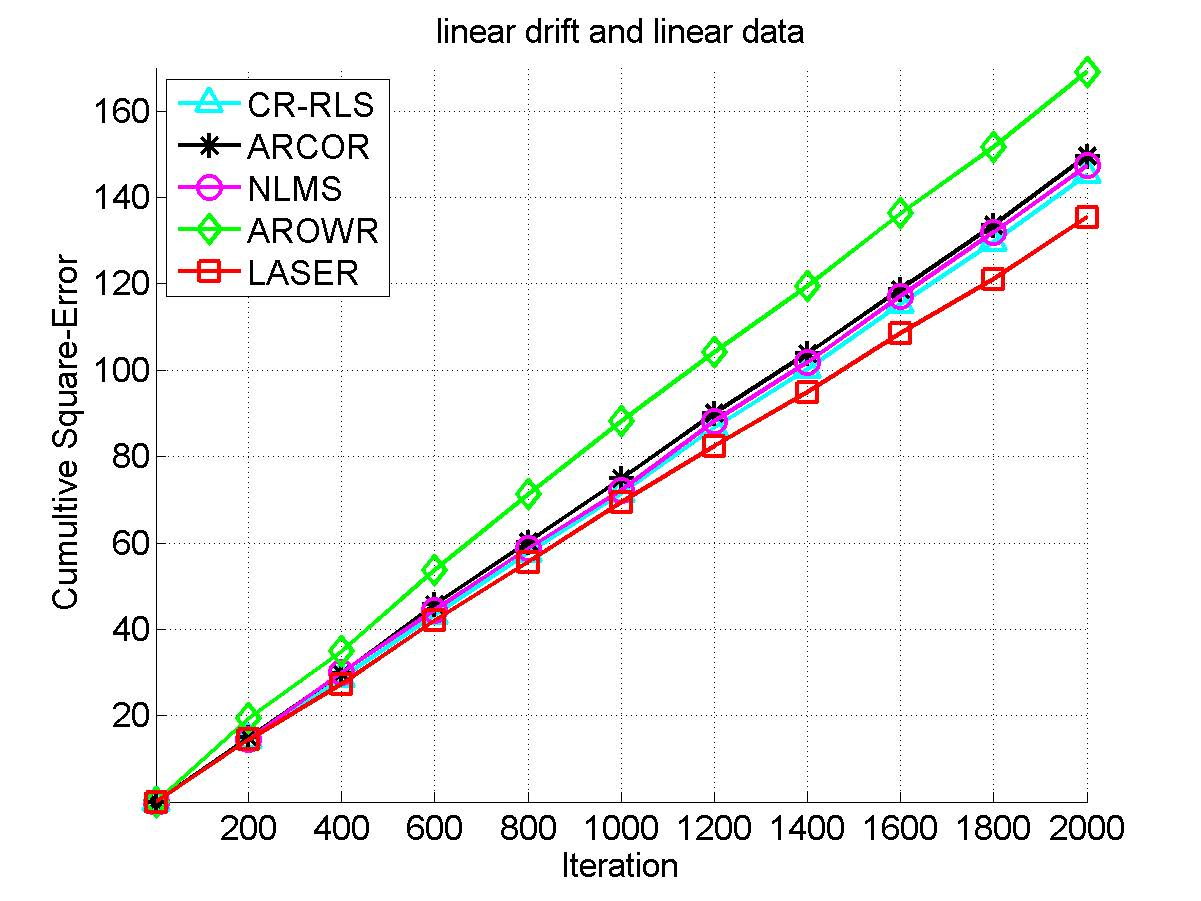
\includegraphics[width=0.50\textwidth]{figs/linear_drift_linear_data.pdf}}
\subfigure{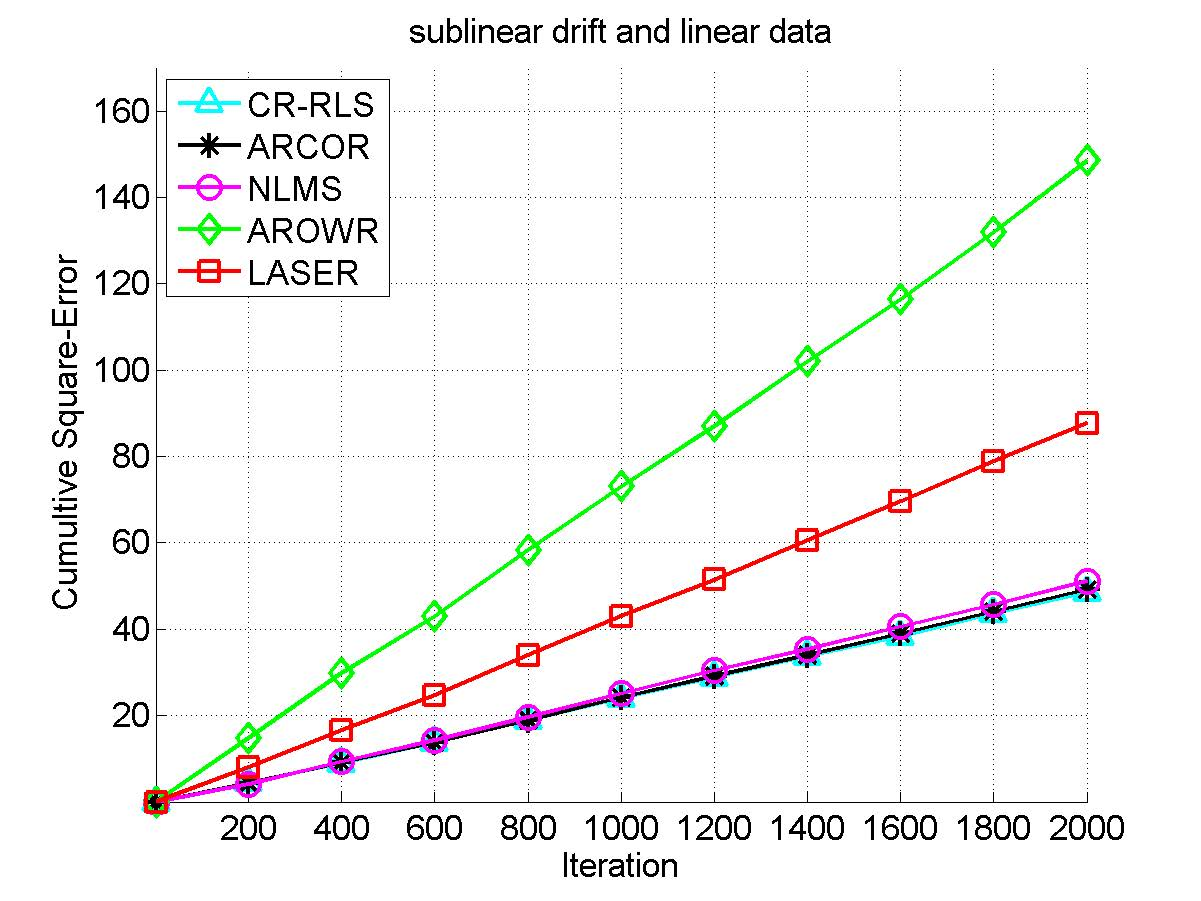
\includegraphics[width=0.50\textwidth]{figs/sublinear_drift_linear_data.pdf}}
\subfigure{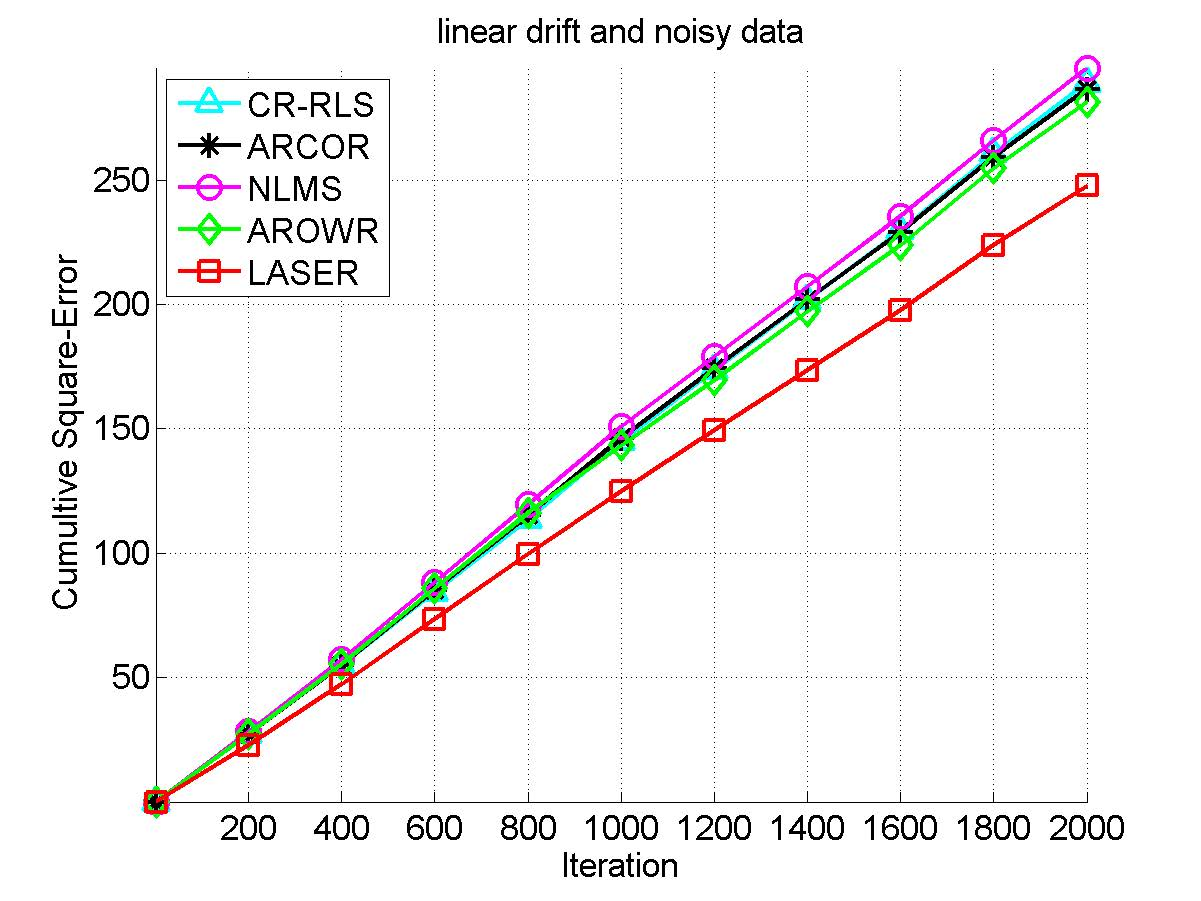
\includegraphics[width=0.50\textwidth]{figs/linear_drift_noisy_data.pdf}}
\subfigure{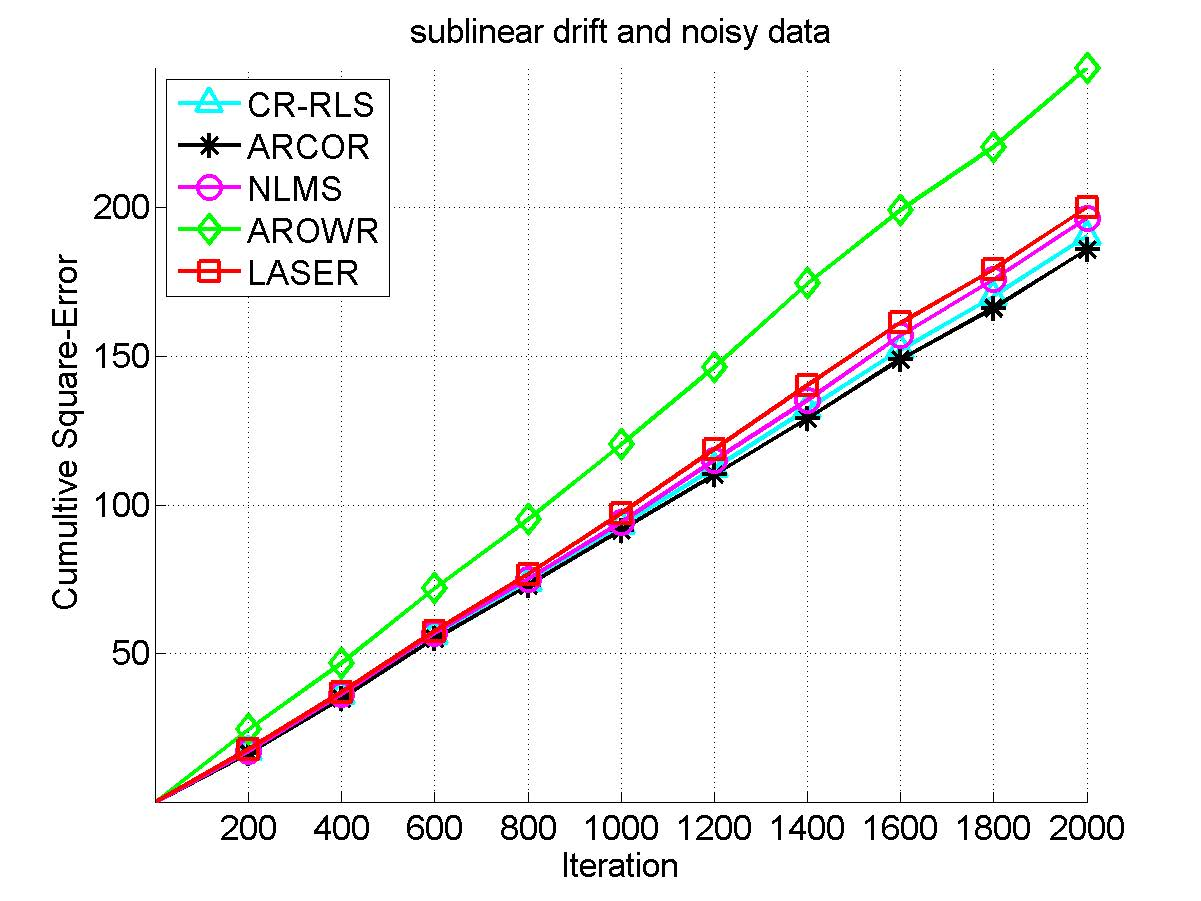
\includegraphics[width=0.50\textwidth]{figs/sublinear_drift_noisy_data.pdf}}
\caption{Cumulative squared loss for NLMS, AROWR, ARCOR,
  CR-RLS and LASER vs iteration. % Top left - linear drift and linear data, top right - sublinear drift and linear data,
  %bottom left - linear drift and noisy data, bottom right - sublinear drift and noisy data.
  }
\label{fig:sims}
\end{figure}
\end{center}
%

The results for the first dataset are summarized in the top-left plot of
\figref{fig:sims}.
For this dataset
AROWR performs the worst, since it converges very fast and does not
allow the ability of tracking changes in data. The ARCOR algorithm for
this dataset performs relatively bad, this is due to the fact that it
is designed for sublinear amount of data drift, while this dataset has
linear drift level, which is the worst case assumed by \texttt{LASER}. CR-RLS
and NLMS show better results, since they both don't make assumptions
on the drift level. CR-RLS performs a little bit better than NLMS
since it has faster learning rate due to the use of second order
information. Finally, LASER %and $H_\infty$
performs the best as expected. It has a good tracking ability, fast learning rate and it is designed to perform well in severe conditions like linear non-stationarity of the data. %, while $H_\infty$ outperforms LASER as expected when the data is close to be linear ($\yi{t}=\vxti{t}\vui{t}$).
Similar results we get for the third dataset (bottom-left plot of \figref{fig:sims}).

For the second and fourth datasets (right plots of
\figref{fig:sims}), where we have sublinear drift level, we get that ARCOR
outperforms \texttt{LASER} since it is especially designed for sublinear amount
of data drift.%, yet, $H_\infty$ outperforms ARCOR.

%For the third and fourth datasets (bottom plots of \figref{fig:sims}), where we added noise to labels, the performance of $H_\infty$ degrades, as expected from our discussion in \chapref{H8_sec}.





\chapter{Related Work}

In the past few years there is a large volume of work on multi-task learning, which clearly we can not 
cover here. The reader is referred to a recent survey on the topic by ~\cite{10.1109/TKDE.2009.191}. 
Most of this work is focused on exploring relations between tasks, that is, 
find similarities and dissimilarities  between tasks, and use it to share data directly ,e.g. 
\cite{NIPS2012_0706}, or model parameters as in ~\cite{Evgeniou:2004:RML:1014052.1014067,Daume:2010:FES:1870526.1870534,DBLP:journals/ml/ArgyriouEP08}. 
In the online settings, there are only a handful of work on multi-task learning. 
~\cite{DBLP:conf/colt/DekelLS06} consider the setting where all algorithms are evaluated using a 
global loss function, and all work towards the shared goal of minimizing it. 
~\cite{DBLP:conf/colt/LugosiPS09}, assume that there are constraints on the predictions of all 
learners, and focus in the expert setting. \cite{Agarwal:EECS-2008-138}, formalize the 
problem in the framework of stochastic convex programming with few matrix regularization, each 
captures some assumption about the relation between the models. 
~\cite{DBLP:journals/jmlr/CavallantiCG10} and ~\cite{cesa2006incremental}, 
assume a known relation between tasks which is exploited during learning. 
Unlike these approaches, we assume the ability to share an annotator rather than data or parameters, 
thus our methods can be applied to problems with no common input space. One can 
expand our algorithm in the case of a related task, and update all the tasks of the model  on each round, 
based on the queried task and not only the queried task.

In the other hand, there are also works that have been done on binary classification with partial feedback . 
Our analysis is derived from ~\cite{cesa2006worst}, yet they focus in selective 
sampling (see also ~\cite{cesa2009robust,dekel2010robust,crammer2014doubly}), that is, making individual 
binary decisions of whether to query, while our algorithm always query, and needs to decide for which task 
to query on each round.
Selective sampling algorithms such as first and second order selective sampling perceptron and   
BBQ  of ~\cite{cesa2006worst,cesa2009robust} deals with binary selective 
sampling algorithms. ~\cite{dekel2010robust} have also a multiple teachers selective sampling 
algorithm, with setting that is similar to SHAMPO with $\kappa$ updates per round , but is force all of the 
inputs to be in the same space.

%Finally, there have been recent work in contextual bandits,~\cite{kakade2008efficient,
%hazan2011newtron,DBLP:journals/ml/CrammerG13}, each with slightly different assumptions. 
%To the best of our knowledge, we are the first to consider decoupled exploration and exploitation in this 
%context. 

~\cite{dietterich1995solving} introduced the use of ECOC matrix to reduce a 
multi-class classification problem into a multi-task problem we use this method, combines with 
SHAMPO algorithms to get multi-class classification. There have been recent work in contextual bandits 
each with slightly different assumptions. Algorithms like contextual bandits such the Banditron of 
~\cite{kakade2008efficient} and Newtron of ~\cite{hazan2011newtron}  used the 
exploration exploitation method in order to reduce the regret, but in their setting, for each round the choice 
is also the prediction, so it suitable to our setting only for the case of One-vs-Rest.
To the best of our knowledge, we are the first to consider decoupled exploration and exploitation in this 
context. 

Finally, there is recent work in learning with relative or preference feedback in various 
settings as in ~\cite{DBLP:conf/colt/YueBKJ09,DBLP:journals/jcss/YueBKJ12,DBLP:conf/icml/YueJ11,DBLP:journals/corr/abs-1111-0712}. 
Unlike this work, our work allows again decoupled exploitation and exploration, and also 
non-relevant feedback.




\chapter{Summary and Conclusions}

We proposed a modification of the last-step min-max algorithm~\citep{Forster} using weights over examples (\texttt{WEMM}), and showed how to choose these weights for the problem to be well defined -- convex -- which enabled us to develop the last-step min-max predictor, without requiring the labels to be bounded. Our algorithmic formulations depend on inner- and outer-products and thus can be employed with kernel functions. Our analysis bounds the regret with quantities that depend only on the loss of the competitor, with no need for any knowledge of the problem.

We also proposed a novel algorithm (\texttt{LASER}) for non-stationary online regression designed and
analyzed with the squared loss. The algorithm was developed from the
last-step min-max predictor for {\em non-stationary} problems, and we
showed an exact recursive form of its solution.
% We also described an algorithm based on the $H_\infty$ filter, that is motivated from a
%min-max approach as well, yet for filtering, and bounded its regret.
 Simulations showed the superior performance of our algorithm, especially in a worst-case (constant per iteration) drift.

An interesting future direction is to extend the algorithms for general loss functions rather than the squared loss, or to classification tasks. Additionally, for the \texttt{LASER}
algorithm to perform well, the amount of drift $V$ or a bound over it
should be known in advance. An interesting direction
is to design algorithms that automatically detect the
level of drift, or do not need this information before run-time.

The derivation of the \texttt{LASER} algorithm does not use the notation of weighted loss. An interesting direction
is to try to incorporate in the derivation of the \texttt{LASER} algorithm the technique of weighted loss used for the derivation of the \texttt{WEMM} algorithm.


%\section*{Appendix}
%\addcontentsline{toc}{section}{Appendix}
%For some reason, you need to manually add stared sections to the the index file.

% Put the path to your bib file (or whatever else you use) here
\clearpage
%\bibliographystyle{fullname}
\bibliographystyle{plainnat}
\bibliography{bib}

% ********************** ADD THIS BACK ********************************
%\include{hebrewPart}
% *********************************************************************

% Actually, I found it much easier to have each chapter in a file of its own. Except for the Hebrew part, I put it all together in this example just to make things clear.

\end{document}
